\documentclass[10pt]{article}
\PassOptionsToPackage{hyphens}{url}

% The Scicom preprint style (scicom.sty): Inter, a mono face and the platform's colours. Build with pdfLaTeX
% (bash build.sh), the engine arXiv runs; bash arxiv.sh makes the upload.
\usepackage{amsmath}
\usepackage{scicom}
\usepackage[authoryear]{natbib}

\usepackage{hyperref}
\usepackage{bookmark}
\usepackage{url}
\usepackage{nicefrac}
\usepackage{microtype}
\usepackage{tabularx}
\usepackage{multirow}
\usepackage{float}
\usepackage{adjustbox}
\usepackage{array}
\usepackage[section]{placeins}

% Floats stay next to the paragraph that introduces them (inherited from the Penjajaran-Daya preprint).
\renewcommand{\topfraction}{0.92}
\renewcommand{\bottomfraction}{0.85}
\renewcommand{\textfraction}{0.06}
\renewcommand{\floatpagefraction}{0.70}
\setcounter{topnumber}{3}
\setcounter{bottomnumber}{2}
\setcounter{totalnumber}{4}
\makeatletter
\setlength{\@fptop}{0pt}
\setlength{\@fpsep}{14pt plus 0fil}
\setlength{\@fpbot}{0pt plus 1fil}
\makeatother
\raggedbottom

\setlength{\textfloatsep}{14pt plus 2pt minus 2pt}
\setlength{\intextsep}{12pt plus 2pt minus 2pt}
\setlength{\floatsep}{14pt plus 2pt minus 2pt}
\setlength{\tabcolsep}{5pt}
\newcolumntype{L}[1]{>{\raggedright\arraybackslash}p{#1}}
% every number in the prose comes from results/ through \val{key} (make_tables.py writes numbers.tex)
% generated by make_tables.py from results/; do not edit
\makeatletter
\newcommand{\val}[1]{\ifcsname v@#1\endcsname\csname v@#1\endcsname\else\textbf{??}\PackageWarning{val}{undefined value #1}\fi}
\expandafter\def\csname v@ami/cough/n\endcsname{78}
\expandafter\def\csname v@ami/cough/nocand_speech\endcsname{56\%}
\expandafter\def\csname v@ami/cough/with_cand\endcsname{29\%}
\expandafter\def\csname v@ami/gap/cough/r\endcsname{0\%}
\expandafter\def\csname v@ami/gap/laugh/p\endcsname{40\%}
\expandafter\def\csname v@ami/gap/laugh/r\endcsname{12\%}
\expandafter\def\csname v@ami/laugh/n\endcsname{763}
\expandafter\def\csname v@ami/laugh/nocand_speech\endcsname{74\%}
\expandafter\def\csname v@ami/laugh/with_cand\endcsname{21\%}
\expandafter\def\csname v@ami/prev/cough/p\endcsname{0\%}
\expandafter\def\csname v@ami/prev/cough/r\endcsname{0\%}
\expandafter\def\csname v@ami/prev/laugh/p\endcsname{81\%}
\expandafter\def\csname v@ami/prev/laugh/r\endcsname{4\%}
\expandafter\def\csname v@as/cough/p\endcsname{80 to 97\%}
\expandafter\def\csname v@as/cough/r\endcsname{17 to 28\%}
\expandafter\def\csname v@as/cough/t\endcsname{0.50}
\expandafter\def\csname v@as/frame/ph\endcsname{18.6}
\expandafter\def\csname v@as/laugh/p\endcsname{84 to 87\%}
\expandafter\def\csname v@as/laugh/r\endcsname{45 to 46\%}
\expandafter\def\csname v@as/laugh/t\endcsname{0.30}
\expandafter\def\csname v@as/nvtts/clips\endcsname{3,970}
\expandafter\def\csname v@as/nvtts/h\endcsname{10.3}
\expandafter\def\csname v@as/sniff/p\endcsname{85 to 88\%}
\expandafter\def\csname v@as/sniff/r\endcsname{68 to 71\%}
\expandafter\def\csname v@as/sniff/t\endcsname{0.15}
\expandafter\def\csname v@as/throat_clear/p\endcsname{81 to 83\%}
\expandafter\def\csname v@as/throat_clear/r\endcsname{34 to 47\%}
\expandafter\def\csname v@as/throat_clear/t\endcsname{0.20}
\expandafter\def\csname v@as/union/p\endcsname{84\%}
\expandafter\def\csname v@as/union/ph\endcsname{26.5}
\expandafter\def\csname v@as/union/r\endcsname{71\%}
\expandafter\def\csname v@as/whisper/found\endcsname{99\%}
\expandafter\def\csname v@as/whisper/n_others\endcsname{10,097}
\expandafter\def\csname v@as/whisper/others\endcsname{0\%}
\expandafter\def\csname v@as/whisper/t\endcsname{0.3}
\expandafter\def\csname v@asr/attn/blank\endcsname{46\%}
\expandafter\def\csname v@asr/attn/clips\endcsname{58,041}
\expandafter\def\csname v@asr/attn/cv22\endcsname{0.385}
\expandafter\def\csname v@asr/attn/cv22_empty\endcsname{5.2\%}
\expandafter\def\csname v@asr/attn/cv22_langs\endcsname{77}
\expandafter\def\csname v@asr/attn/cv22_pool_langs\endcsname{77}
\expandafter\def\csname v@asr/attn/det\endcsname{0.451}
\expandafter\def\csname v@asr/attn/det_failed\endcsname{425}
\expandafter\def\csname v@asr/attn/fleurs\endcsname{0.451}
\expandafter\def\csname v@asr/attn/fleurs_empty\endcsname{25.7\%}
\expandafter\def\csname v@asr/attn/fleurs_empty_langs\endcsname{51}
\expandafter\def\csname v@asr/attn/fleurs_empty_max\endcsname{85\%}
\expandafter\def\csname v@asr/attn/fleurs_empty_top\endcsname{Japanese (85\%), Khmer (80\%), Burmese (75\%) and Shona (70\%)}
\expandafter\def\csname v@asr/attn/fleurs_langs\endcsname{58}
\expandafter\def\csname v@asr/attn/forced\endcsname{0.422}
\expandafter\def\csname v@asr/attn/forced_failed\endcsname{369}
\expandafter\def\csname v@asr/attn/genuine_wer\endcsname{22.0\%}
\expandafter\def\csname v@asr/attn/genuine_wer_clipmean\endcsname{31.2\%}
\expandafter\def\csname v@asr/attn/lexicon_recovered\endcsname{71.8\%}
\expandafter\def\csname v@asr/attn/librispeech_wer\endcsname{3.52\%}
\expandafter\def\csname v@asr/attn/lid_acc\endcsname{78.1\%}
\expandafter\def\csname v@asr/attn/ls_empty\endcsname{0.2\%}
\expandafter\def\csname v@asr/attn/mix_hours\endcsname{131}
\expandafter\def\csname v@asr/attn/mix_langs\endcsname{75}
\expandafter\def\csname v@asr/attn/music_hr\endcsname{0.2\%}
\expandafter\def\csname v@asr/attn/my_empty\endcsname{2.5\%}
\expandafter\def\csname v@asr/attn/noise0\endcsname{22.5\%}
\expandafter\def\csname v@asr/attn/noise20\endcsname{5.0\%}
\expandafter\def\csname v@asr/attn/noise_empty\endcsname{16.8\%}
\expandafter\def\csname v@asr/attn/noisem5\endcsname{34.6\%}
\expandafter\def\csname v@asr/attn/nonspeech_hr\endcsname{0.2\%}
\expandafter\def\csname v@asr/attn/redup_empty\endcsname{6.7\%}
\expandafter\def\csname v@asr/attn/runaway\endcsname{0.8\%}
\expandafter\def\csname v@asr/attn/silence_hr\endcsname{0.0\%}
\expandafter\def\csname v@asr/attn/wild_words\endcsname{1.5\%}
\expandafter\def\csname v@asr/base/cv22\endcsname{0.353}
\expandafter\def\csname v@asr/base/cv22_empty\endcsname{0.1\%}
\expandafter\def\csname v@asr/base/cv22_langs\endcsname{77}
\expandafter\def\csname v@asr/base/det\endcsname{0.282}
\expandafter\def\csname v@asr/base/det_failed\endcsname{156}
\expandafter\def\csname v@asr/base/fleurs\endcsname{0.282}
\expandafter\def\csname v@asr/base/fleurs_empty\endcsname{0.0\%}
\expandafter\def\csname v@asr/base/fleurs_empty_langs\endcsname{0}
\expandafter\def\csname v@asr/base/fleurs_empty_max\endcsname{0\%}
\expandafter\def\csname v@asr/base/fleurs_langs\endcsname{58}
\expandafter\def\csname v@asr/base/forced\endcsname{0.259}
\expandafter\def\csname v@asr/base/forced_failed\endcsname{118}
\expandafter\def\csname v@asr/base/genuine_wer\endcsname{23.4\%}
\expandafter\def\csname v@asr/base/genuine_wer_clipmean\endcsname{32.1\%}
\expandafter\def\csname v@asr/base/lexicon_recovered\endcsname{67.9\%}
\expandafter\def\csname v@asr/base/librispeech_wer\endcsname{3.06\%}
\expandafter\def\csname v@asr/base/lid_acc\endcsname{83.7\%}
\expandafter\def\csname v@asr/base/ls_empty\endcsname{0.0\%}
\expandafter\def\csname v@asr/base/music_hr\endcsname{99.0\%}
\expandafter\def\csname v@asr/base/my_empty\endcsname{0.0\%}
\expandafter\def\csname v@asr/base/noise0\endcsname{0.0\%}
\expandafter\def\csname v@asr/base/noise20\endcsname{0.0\%}
\expandafter\def\csname v@asr/base/noise_empty\endcsname{0.0\%}
\expandafter\def\csname v@asr/base/noisem5\endcsname{0.0\%}
\expandafter\def\csname v@asr/base/nonspeech_hr\endcsname{97.3\%}
\expandafter\def\csname v@asr/base/redup_empty\endcsname{0.1\%}
\expandafter\def\csname v@asr/base/runaway\endcsname{1.4\%}
\expandafter\def\csname v@asr/base/silence_hr\endcsname{61.9\%}
\expandafter\def\csname v@asr/base/wild_words\endcsname{99.9\%}
\expandafter\def\csname v@asr/blank_en\endcsname{76\%}
\expandafter\def\csname v@asr/blank_n\endcsname{26,510}
\expandafter\def\csname v@asr/bug/blank\endcsname{46\%}
\expandafter\def\csname v@asr/bug/clips\endcsname{58,041}
\expandafter\def\csname v@asr/bug/cv22\endcsname{0.435}
\expandafter\def\csname v@asr/bug/cv22_empty\endcsname{0.5\%}
\expandafter\def\csname v@asr/bug/cv22_langs\endcsname{77}
\expandafter\def\csname v@asr/bug/cv22_pool_langs\endcsname{77}
\expandafter\def\csname v@asr/bug/det\endcsname{0.354}
\expandafter\def\csname v@asr/bug/det_failed\endcsname{220}
\expandafter\def\csname v@asr/bug/fleurs\endcsname{0.354}
\expandafter\def\csname v@asr/bug/fleurs_empty\endcsname{0.4\%}
\expandafter\def\csname v@asr/bug/fleurs_empty_langs\endcsname{3}
\expandafter\def\csname v@asr/bug/fleurs_empty_max\endcsname{15\%}
\expandafter\def\csname v@asr/bug/fleurs_empty_top\endcsname{Hausa (15\%), English (5\%) and Punjabi (5\%)}
\expandafter\def\csname v@asr/bug/fleurs_langs\endcsname{58}
\expandafter\def\csname v@asr/bug/forced\endcsname{0.292}
\expandafter\def\csname v@asr/bug/forced_failed\endcsname{168}
\expandafter\def\csname v@asr/bug/genuine_wer\endcsname{24.1\%}
\expandafter\def\csname v@asr/bug/genuine_wer_clipmean\endcsname{36.8\%}
\expandafter\def\csname v@asr/bug/lexicon_recovered\endcsname{77.9\%}
\expandafter\def\csname v@asr/bug/librispeech_wer\endcsname{3.26\%}
\expandafter\def\csname v@asr/bug/lid_acc\endcsname{77.2\%}
\expandafter\def\csname v@asr/bug/ls_empty\endcsname{0.0\%}
\expandafter\def\csname v@asr/bug/mix_hours\endcsname{131}
\expandafter\def\csname v@asr/bug/mix_langs\endcsname{75}
\expandafter\def\csname v@asr/bug/music_hr\endcsname{6.8\%}
\expandafter\def\csname v@asr/bug/my_empty\endcsname{0.2\%}
\expandafter\def\csname v@asr/bug/noise0\endcsname{4.6\%}
\expandafter\def\csname v@asr/bug/noise20\endcsname{0.4\%}
\expandafter\def\csname v@asr/bug/noise_empty\endcsname{3.1\%}
\expandafter\def\csname v@asr/bug/noisem5\endcsname{7.9\%}
\expandafter\def\csname v@asr/bug/nonspeech_hr\endcsname{0.9\%}
\expandafter\def\csname v@asr/bug/redup_empty\endcsname{10.1\%}
\expandafter\def\csname v@asr/bug/runaway\endcsname{3.5\%}
\expandafter\def\csname v@asr/bug/silence_hr\endcsname{33.3\%}
\expandafter\def\csname v@asr/bug/wild_words\endcsname{12.8\%}
\expandafter\def\csname v@asr/d25bl/blank\endcsname{34\%}
\expandafter\def\csname v@asr/d25bl/clips\endcsname{77,388}
\expandafter\def\csname v@asr/d25bl/cv22\endcsname{0.323}
\expandafter\def\csname v@asr/d25bl/cv22_empty\endcsname{0.4\%}
\expandafter\def\csname v@asr/d25bl/cv22_langs\endcsname{77}
\expandafter\def\csname v@asr/d25bl/cv22_pool_langs\endcsname{77}
\expandafter\def\csname v@asr/d25bl/det\endcsname{0.274}
\expandafter\def\csname v@asr/d25bl/det_failed\endcsname{157}
\expandafter\def\csname v@asr/d25bl/fleurs\endcsname{0.274}
\expandafter\def\csname v@asr/d25bl/fleurs_empty\endcsname{0.9\%}
\expandafter\def\csname v@asr/d25bl/fleurs_empty_langs\endcsname{6}
\expandafter\def\csname v@asr/d25bl/fleurs_empty_max\endcsname{20\%}
\expandafter\def\csname v@asr/d25bl/fleurs_empty_top\endcsname{Japanese (20\%), Vietnamese (10\%), German (5\%) and French (5\%)}
\expandafter\def\csname v@asr/d25bl/fleurs_langs\endcsname{58}
\expandafter\def\csname v@asr/d25bl/forced\endcsname{0.250}
\expandafter\def\csname v@asr/d25bl/forced_failed\endcsname{96}
\expandafter\def\csname v@asr/d25bl/genuine_wer\endcsname{22.6\%}
\expandafter\def\csname v@asr/d25bl/genuine_wer_clipmean\endcsname{31.9\%}
\expandafter\def\csname v@asr/d25bl/lexicon_recovered\endcsname{69.7\%}
\expandafter\def\csname v@asr/d25bl/librispeech_wer\endcsname{8.42\%}
\expandafter\def\csname v@asr/d25bl/lid_acc\endcsname{83.5\%}
\expandafter\def\csname v@asr/d25bl/ls_empty\endcsname{3.8\%}
\expandafter\def\csname v@asr/d25bl/mix_hours\endcsname{157}
\expandafter\def\csname v@asr/d25bl/mix_langs\endcsname{89}
\expandafter\def\csname v@asr/d25bl/music_hr\endcsname{0.2\%}
\expandafter\def\csname v@asr/d25bl/my_empty\endcsname{1.6\%}
\expandafter\def\csname v@asr/d25bl/noise0\endcsname{5.4\%}
\expandafter\def\csname v@asr/d25bl/noise20\endcsname{1.2\%}
\expandafter\def\csname v@asr/d25bl/noise_empty\endcsname{5.6\%}
\expandafter\def\csname v@asr/d25bl/noisem5\endcsname{15.0\%}
\expandafter\def\csname v@asr/d25bl/nonspeech_hr\endcsname{0.1\%}
\expandafter\def\csname v@asr/d25bl/redup_empty\endcsname{12.5\%}
\expandafter\def\csname v@asr/d25bl/runaway\endcsname{9.2\%}
\expandafter\def\csname v@asr/d25bl/silence_hr\endcsname{0.0\%}
\expandafter\def\csname v@asr/d25bl/wild_words\endcsname{0.5\%}
\expandafter\def\csname v@asr/distill/blank\endcsname{46\%}
\expandafter\def\csname v@asr/distill/clips\endcsname{58,041}
\expandafter\def\csname v@asr/distill/cv22\endcsname{0.381}
\expandafter\def\csname v@asr/distill/cv22_empty\endcsname{3.4\%}
\expandafter\def\csname v@asr/distill/cv22_langs\endcsname{77}
\expandafter\def\csname v@asr/distill/cv22_pool_langs\endcsname{77}
\expandafter\def\csname v@asr/distill/det\endcsname{0.434}
\expandafter\def\csname v@asr/distill/det_failed\endcsname{395}
\expandafter\def\csname v@asr/distill/fleurs\endcsname{0.434}
\expandafter\def\csname v@asr/distill/fleurs_empty\endcsname{23.4\%}
\expandafter\def\csname v@asr/distill/fleurs_empty_langs\endcsname{46}
\expandafter\def\csname v@asr/distill/fleurs_empty_max\endcsname{100\%}
\expandafter\def\csname v@asr/distill/fleurs_empty_top\endcsname{Burmese (100\%), Khmer (80\%), Japanese (70\%) and Malayalam (70\%)}
\expandafter\def\csname v@asr/distill/fleurs_langs\endcsname{58}
\expandafter\def\csname v@asr/distill/forced\endcsname{0.424}
\expandafter\def\csname v@asr/distill/forced_failed\endcsname{363}
\expandafter\def\csname v@asr/distill/genuine_wer\endcsname{23.9\%}
\expandafter\def\csname v@asr/distill/genuine_wer_clipmean\endcsname{33.5\%}
\expandafter\def\csname v@asr/distill/lexicon_recovered\endcsname{70.0\%}
\expandafter\def\csname v@asr/distill/librispeech_wer\endcsname{3.32\%}
\expandafter\def\csname v@asr/distill/lid_acc\endcsname{82.8\%}
\expandafter\def\csname v@asr/distill/ls_empty\endcsname{0.1\%}
\expandafter\def\csname v@asr/distill/mix_hours\endcsname{131}
\expandafter\def\csname v@asr/distill/mix_langs\endcsname{75}
\expandafter\def\csname v@asr/distill/music_hr\endcsname{1.7\%}
\expandafter\def\csname v@asr/distill/my_empty\endcsname{1.7\%}
\expandafter\def\csname v@asr/distill/noise0\endcsname{15.8\%}
\expandafter\def\csname v@asr/distill/noise20\endcsname{2.1\%}
\expandafter\def\csname v@asr/distill/noise_empty\endcsname{10.9\%}
\expandafter\def\csname v@asr/distill/noisem5\endcsname{22.9\%}
\expandafter\def\csname v@asr/distill/nonspeech_hr\endcsname{0.2\%}
\expandafter\def\csname v@asr/distill/redup_empty\endcsname{10.0\%}
\expandafter\def\csname v@asr/distill/runaway\endcsname{2.3\%}
\expandafter\def\csname v@asr/distill/silence_hr\endcsname{0.0\%}
\expandafter\def\csname v@asr/distill/wild_words\endcsname{5.1\%}
\expandafter\def\csname v@asr/distill25/blank\endcsname{34\%}
\expandafter\def\csname v@asr/distill25/clips\endcsname{77,388}
\expandafter\def\csname v@asr/distill25/cv22\endcsname{0.342}
\expandafter\def\csname v@asr/distill25/cv22_empty\endcsname{0.2\%}
\expandafter\def\csname v@asr/distill25/cv22_langs\endcsname{77}
\expandafter\def\csname v@asr/distill25/cv22_pool_langs\endcsname{77}
\expandafter\def\csname v@asr/distill25/det\endcsname{0.285}
\expandafter\def\csname v@asr/distill25/det_failed\endcsname{162}
\expandafter\def\csname v@asr/distill25/fleurs\endcsname{0.285}
\expandafter\def\csname v@asr/distill25/fleurs_empty\endcsname{0.3\%}
\expandafter\def\csname v@asr/distill25/fleurs_empty_langs\endcsname{3}
\expandafter\def\csname v@asr/distill25/fleurs_empty_max\endcsname{5\%}
\expandafter\def\csname v@asr/distill25/fleurs_empty_top\endcsname{German (5\%), Japanese (5\%) and Khmer (5\%)}
\expandafter\def\csname v@asr/distill25/fleurs_langs\endcsname{58}
\expandafter\def\csname v@asr/distill25/forced\endcsname{0.238}
\expandafter\def\csname v@asr/distill25/forced_failed\endcsname{89}
\expandafter\def\csname v@asr/distill25/genuine_wer\endcsname{22.9\%}
\expandafter\def\csname v@asr/distill25/genuine_wer_clipmean\endcsname{33.2\%}
\expandafter\def\csname v@asr/distill25/lexicon_recovered\endcsname{69.9\%}
\expandafter\def\csname v@asr/distill25/librispeech_wer\endcsname{3.17\%}
\expandafter\def\csname v@asr/distill25/lid_acc\endcsname{82.3\%}
\expandafter\def\csname v@asr/distill25/ls_empty\endcsname{0.1\%}
\expandafter\def\csname v@asr/distill25/mix_hours\endcsname{157}
\expandafter\def\csname v@asr/distill25/mix_langs\endcsname{89}
\expandafter\def\csname v@asr/distill25/music_hr\endcsname{1.0\%}
\expandafter\def\csname v@asr/distill25/my_empty\endcsname{0.8\%}
\expandafter\def\csname v@asr/distill25/noise0\endcsname{7.9\%}
\expandafter\def\csname v@asr/distill25/noise20\endcsname{0.8\%}
\expandafter\def\csname v@asr/distill25/noise_empty\endcsname{6.3\%}
\expandafter\def\csname v@asr/distill25/noisem5\endcsname{18.3\%}
\expandafter\def\csname v@asr/distill25/nonspeech_hr\endcsname{0.0\%}
\expandafter\def\csname v@asr/distill25/redup_empty\endcsname{13.5\%}
\expandafter\def\csname v@asr/distill25/runaway\endcsname{13.8\%}
\expandafter\def\csname v@asr/distill25/silence_hr\endcsname{0.0\%}
\expandafter\def\csname v@asr/distill25/wild_words\endcsname{2.4\%}
\expandafter\def\csname v@asr/fix/blank\endcsname{46\%}
\expandafter\def\csname v@asr/fix/clips\endcsname{58,041}
\expandafter\def\csname v@asr/fix/cv22\endcsname{0.406}
\expandafter\def\csname v@asr/fix/cv22_empty\endcsname{6.1\%}
\expandafter\def\csname v@asr/fix/cv22_langs\endcsname{77}
\expandafter\def\csname v@asr/fix/cv22_pool_langs\endcsname{77}
\expandafter\def\csname v@asr/fix/det\endcsname{0.484}
\expandafter\def\csname v@asr/fix/det_failed\endcsname{469}
\expandafter\def\csname v@asr/fix/fleurs\endcsname{0.484}
\expandafter\def\csname v@asr/fix/fleurs_empty\endcsname{29.6\%}
\expandafter\def\csname v@asr/fix/fleurs_empty_langs\endcsname{51}
\expandafter\def\csname v@asr/fix/fleurs_empty_max\endcsname{95\%}
\expandafter\def\csname v@asr/fix/fleurs_empty_top\endcsname{Japanese (95\%), Shona (95\%), Burmese (90\%) and Yoruba (90\%)}
\expandafter\def\csname v@asr/fix/fleurs_langs\endcsname{58}
\expandafter\def\csname v@asr/fix/forced\endcsname{0.455}
\expandafter\def\csname v@asr/fix/forced_failed\endcsname{420}
\expandafter\def\csname v@asr/fix/genuine_wer\endcsname{24.4\%}
\expandafter\def\csname v@asr/fix/genuine_wer_clipmean\endcsname{35.9\%}
\expandafter\def\csname v@asr/fix/lexicon_recovered\endcsname{72.4\%}
\expandafter\def\csname v@asr/fix/librispeech_wer\endcsname{4.21\%}
\expandafter\def\csname v@asr/fix/lid_acc\endcsname{77.2\%}
\expandafter\def\csname v@asr/fix/ls_empty\endcsname{0.5\%}
\expandafter\def\csname v@asr/fix/mix_hours\endcsname{131}
\expandafter\def\csname v@asr/fix/mix_langs\endcsname{75}
\expandafter\def\csname v@asr/fix/music_hr\endcsname{0.3\%}
\expandafter\def\csname v@asr/fix/my_empty\endcsname{3.0\%}
\expandafter\def\csname v@asr/fix/noise0\endcsname{20.8\%}
\expandafter\def\csname v@asr/fix/noise20\endcsname{4.2\%}
\expandafter\def\csname v@asr/fix/noise_empty\endcsname{15.2\%}
\expandafter\def\csname v@asr/fix/noisem5\endcsname{31.2\%}
\expandafter\def\csname v@asr/fix/nonspeech_hr\endcsname{0.2\%}
\expandafter\def\csname v@asr/fix/redup_empty\endcsname{10.3\%}
\expandafter\def\csname v@asr/fix/runaway\endcsname{4.1\%}
\expandafter\def\csname v@asr/fix/silence_hr\endcsname{0.0\%}
\expandafter\def\csname v@asr/fix/wild_words\endcsname{0.9\%}
\expandafter\def\csname v@asr/fix25/blank\endcsname{34\%}
\expandafter\def\csname v@asr/fix25/clips\endcsname{77,388}
\expandafter\def\csname v@asr/fix25/cv22\endcsname{0.333}
\expandafter\def\csname v@asr/fix25/cv22_empty\endcsname{0.2\%}
\expandafter\def\csname v@asr/fix25/cv22_langs\endcsname{77}
\expandafter\def\csname v@asr/fix25/cv22_pool_langs\endcsname{77}
\expandafter\def\csname v@asr/fix25/det\endcsname{0.294}
\expandafter\def\csname v@asr/fix25/det_failed\endcsname{186}
\expandafter\def\csname v@asr/fix25/fleurs\endcsname{0.294}
\expandafter\def\csname v@asr/fix25/fleurs_empty\endcsname{0.1\%}
\expandafter\def\csname v@asr/fix25/fleurs_empty_langs\endcsname{1}
\expandafter\def\csname v@asr/fix25/fleurs_empty_max\endcsname{5\%}
\expandafter\def\csname v@asr/fix25/fleurs_empty_top\endcsname{Khmer (5\%)}
\expandafter\def\csname v@asr/fix25/fleurs_langs\endcsname{58}
\expandafter\def\csname v@asr/fix25/forced\endcsname{0.235}
\expandafter\def\csname v@asr/fix25/forced_failed\endcsname{85}
\expandafter\def\csname v@asr/fix25/genuine_wer\endcsname{22.9\%}
\expandafter\def\csname v@asr/fix25/genuine_wer_clipmean\endcsname{32.9\%}
\expandafter\def\csname v@asr/fix25/lexicon_recovered\endcsname{69.5\%}
\expandafter\def\csname v@asr/fix25/librispeech_wer\endcsname{3.03\%}
\expandafter\def\csname v@asr/fix25/lid_acc\endcsname{72.0\%}
\expandafter\def\csname v@asr/fix25/ls_empty\endcsname{0.0\%}
\expandafter\def\csname v@asr/fix25/mix_hours\endcsname{157}
\expandafter\def\csname v@asr/fix25/mix_langs\endcsname{89}
\expandafter\def\csname v@asr/fix25/music_hr\endcsname{1.0\%}
\expandafter\def\csname v@asr/fix25/my_empty\endcsname{0.9\%}
\expandafter\def\csname v@asr/fix25/noise0\endcsname{4.2\%}
\expandafter\def\csname v@asr/fix25/noise20\endcsname{0.4\%}
\expandafter\def\csname v@asr/fix25/noise_empty\endcsname{4.8\%}
\expandafter\def\csname v@asr/fix25/noisem5\endcsname{14.2\%}
\expandafter\def\csname v@asr/fix25/nonspeech_hr\endcsname{0.3\%}
\expandafter\def\csname v@asr/fix25/redup_empty\endcsname{10.1\%}
\expandafter\def\csname v@asr/fix25/runaway\endcsname{3.1\%}
\expandafter\def\csname v@asr/fix25/silence_hr\endcsname{0.0\%}
\expandafter\def\csname v@asr/fix25/wild_words\endcsname{4.3\%}
\expandafter\def\csname v@asr/fix50/blank\endcsname{23\%}
\expandafter\def\csname v@asr/fix50/clips\endcsname{116,082}
\expandafter\def\csname v@asr/fix50/cv22\endcsname{0.326}
\expandafter\def\csname v@asr/fix50/cv22_empty\endcsname{0.1\%}
\expandafter\def\csname v@asr/fix50/cv22_langs\endcsname{77}
\expandafter\def\csname v@asr/fix50/cv22_pool_langs\endcsname{77}
\expandafter\def\csname v@asr/fix50/det\endcsname{0.299}
\expandafter\def\csname v@asr/fix50/det_failed\endcsname{198}
\expandafter\def\csname v@asr/fix50/fleurs\endcsname{0.299}
\expandafter\def\csname v@asr/fix50/fleurs_empty\endcsname{0.3\%}
\expandafter\def\csname v@asr/fix50/fleurs_empty_langs\endcsname{4}
\expandafter\def\csname v@asr/fix50/fleurs_empty_max\endcsname{5\%}
\expandafter\def\csname v@asr/fix50/fleurs_empty_top\endcsname{Hausa (5\%), Khmer (5\%), Burmese (5\%) and Pashto (5\%)}
\expandafter\def\csname v@asr/fix50/fleurs_langs\endcsname{58}
\expandafter\def\csname v@asr/fix50/forced\endcsname{0.216}
\expandafter\def\csname v@asr/fix50/forced_failed\endcsname{92}
\expandafter\def\csname v@asr/fix50/genuine_wer\endcsname{21.9\%}
\expandafter\def\csname v@asr/fix50/genuine_wer_clipmean\endcsname{31.3\%}
\expandafter\def\csname v@asr/fix50/lexicon_recovered\endcsname{68.0\%}
\expandafter\def\csname v@asr/fix50/librispeech_wer\endcsname{3.21\%}
\expandafter\def\csname v@asr/fix50/lid_acc\endcsname{74.3\%}
\expandafter\def\csname v@asr/fix50/ls_empty\endcsname{0.1\%}
\expandafter\def\csname v@asr/fix50/mix_hours\endcsname{210}
\expandafter\def\csname v@asr/fix50/mix_langs\endcsname{89}
\expandafter\def\csname v@asr/fix50/music_hr\endcsname{1.2\%}
\expandafter\def\csname v@asr/fix50/my_empty\endcsname{1.8\%}
\expandafter\def\csname v@asr/fix50/noise0\endcsname{6.7\%}
\expandafter\def\csname v@asr/fix50/noise20\endcsname{2.1\%}
\expandafter\def\csname v@asr/fix50/noise_empty\endcsname{6.2\%}
\expandafter\def\csname v@asr/fix50/noisem5\endcsname{14.2\%}
\expandafter\def\csname v@asr/fix50/nonspeech_hr\endcsname{0.3\%}
\expandafter\def\csname v@asr/fix50/redup_empty\endcsname{13.3\%}
\expandafter\def\csname v@asr/fix50/runaway\endcsname{11.3\%}
\expandafter\def\csname v@asr/fix50/silence_hr\endcsname{0.0\%}
\expandafter\def\csname v@asr/fix50/wild_words\endcsname{1.9\%}
\expandafter\def\csname v@asr/fleurs_clips\endcsname{1,160}
\expandafter\def\csname v@asr/fleurs_langs\endcsname{58}
\expandafter\def\csname v@asr/full2e-5/blank\endcsname{46\%}
\expandafter\def\csname v@asr/full2e-5/clips\endcsname{58,041}
\expandafter\def\csname v@asr/full2e-5/cv22\endcsname{0.386}
\expandafter\def\csname v@asr/full2e-5/cv22_empty\endcsname{3.7\%}
\expandafter\def\csname v@asr/full2e-5/cv22_langs\endcsname{77}
\expandafter\def\csname v@asr/full2e-5/cv22_pool_langs\endcsname{77}
\expandafter\def\csname v@asr/full2e-5/det\endcsname{0.350}
\expandafter\def\csname v@asr/full2e-5/det_failed\endcsname{259}
\expandafter\def\csname v@asr/full2e-5/fleurs\endcsname{0.350}
\expandafter\def\csname v@asr/full2e-5/fleurs_empty\endcsname{7.9\%}
\expandafter\def\csname v@asr/full2e-5/fleurs_empty_langs\endcsname{25}
\expandafter\def\csname v@asr/full2e-5/fleurs_empty_max\endcsname{50\%}
\expandafter\def\csname v@asr/full2e-5/fleurs_empty_top\endcsname{Japanese (50\%), Khmer (50\%), Burmese (45\%) and Yoruba (45\%)}
\expandafter\def\csname v@asr/full2e-5/fleurs_langs\endcsname{58}
\expandafter\def\csname v@asr/full2e-5/forced\endcsname{0.316}
\expandafter\def\csname v@asr/full2e-5/forced_failed\endcsname{208}
\expandafter\def\csname v@asr/full2e-5/genuine_wer\endcsname{23.0\%}
\expandafter\def\csname v@asr/full2e-5/genuine_wer_clipmean\endcsname{32.1\%}
\expandafter\def\csname v@asr/full2e-5/lexicon_recovered\endcsname{73.5\%}
\expandafter\def\csname v@asr/full2e-5/librispeech_wer\endcsname{3.04\%}
\expandafter\def\csname v@asr/full2e-5/lid_acc\endcsname{82.2\%}
\expandafter\def\csname v@asr/full2e-5/ls_empty\endcsname{0.0\%}
\expandafter\def\csname v@asr/full2e-5/mix_hours\endcsname{131}
\expandafter\def\csname v@asr/full2e-5/mix_langs\endcsname{75}
\expandafter\def\csname v@asr/full2e-5/music_hr\endcsname{0.7\%}
\expandafter\def\csname v@asr/full2e-5/my_empty\endcsname{1.8\%}
\expandafter\def\csname v@asr/full2e-5/noise0\endcsname{17.5\%}
\expandafter\def\csname v@asr/full2e-5/noise20\endcsname{4.6\%}
\expandafter\def\csname v@asr/full2e-5/noise_empty\endcsname{14.4\%}
\expandafter\def\csname v@asr/full2e-5/noisem5\endcsname{33.3\%}
\expandafter\def\csname v@asr/full2e-5/nonspeech_hr\endcsname{0.0\%}
\expandafter\def\csname v@asr/full2e-5/redup_empty\endcsname{14.4\%}
\expandafter\def\csname v@asr/full2e-5/runaway\endcsname{0.0\%}
\expandafter\def\csname v@asr/full2e-5/silence_hr\endcsname{0.0\%}
\expandafter\def\csname v@asr/full2e-5/wild_words\endcsname{4.2\%}
\expandafter\def\csname v@asr/full5e-6/blank\endcsname{46\%}
\expandafter\def\csname v@asr/full5e-6/clips\endcsname{58,041}
\expandafter\def\csname v@asr/full5e-6/cv22\endcsname{0.351}
\expandafter\def\csname v@asr/full5e-6/cv22_empty\endcsname{3.6\%}
\expandafter\def\csname v@asr/full5e-6/cv22_langs\endcsname{77}
\expandafter\def\csname v@asr/full5e-6/cv22_pool_langs\endcsname{77}
\expandafter\def\csname v@asr/full5e-6/det\endcsname{0.307}
\expandafter\def\csname v@asr/full5e-6/det_failed\endcsname{218}
\expandafter\def\csname v@asr/full5e-6/fleurs\endcsname{0.307}
\expandafter\def\csname v@asr/full5e-6/fleurs_empty\endcsname{7.7\%}
\expandafter\def\csname v@asr/full5e-6/fleurs_empty_langs\endcsname{33}
\expandafter\def\csname v@asr/full5e-6/fleurs_empty_max\endcsname{65\%}
\expandafter\def\csname v@asr/full5e-6/fleurs_empty_top\endcsname{Khmer (65\%), Somali (55\%), Hausa (35\%) and Japanese (35\%)}
\expandafter\def\csname v@asr/full5e-6/fleurs_langs\endcsname{58}
\expandafter\def\csname v@asr/full5e-6/forced\endcsname{0.283}
\expandafter\def\csname v@asr/full5e-6/forced_failed\endcsname{175}
\expandafter\def\csname v@asr/full5e-6/genuine_wer\endcsname{22.3\%}
\expandafter\def\csname v@asr/full5e-6/genuine_wer_clipmean\endcsname{32.5\%}
\expandafter\def\csname v@asr/full5e-6/lexicon_recovered\endcsname{73.2\%}
\expandafter\def\csname v@asr/full5e-6/librispeech_wer\endcsname{2.89\%}
\expandafter\def\csname v@asr/full5e-6/lid_acc\endcsname{83.9\%}
\expandafter\def\csname v@asr/full5e-6/ls_empty\endcsname{0.0\%}
\expandafter\def\csname v@asr/full5e-6/mix_hours\endcsname{131}
\expandafter\def\csname v@asr/full5e-6/mix_langs\endcsname{75}
\expandafter\def\csname v@asr/full5e-6/music_hr\endcsname{1.2\%}
\expandafter\def\csname v@asr/full5e-6/my_empty\endcsname{2.2\%}
\expandafter\def\csname v@asr/full5e-6/noise0\endcsname{16.2\%}
\expandafter\def\csname v@asr/full5e-6/noise20\endcsname{3.3\%}
\expandafter\def\csname v@asr/full5e-6/noise_empty\endcsname{12.1\%}
\expandafter\def\csname v@asr/full5e-6/noisem5\endcsname{25.8\%}
\expandafter\def\csname v@asr/full5e-6/nonspeech_hr\endcsname{0.0\%}
\expandafter\def\csname v@asr/full5e-6/redup_empty\endcsname{20.1\%}
\expandafter\def\csname v@asr/full5e-6/runaway\endcsname{0.8\%}
\expandafter\def\csname v@asr/full5e-6/silence_hr\endcsname{0.0\%}
\expandafter\def\csname v@asr/full5e-6/wild_words\endcsname{3.6\%}
\expandafter\def\csname v@asr/label/blank\endcsname{46\%}
\expandafter\def\csname v@asr/label/clips\endcsname{58,041}
\expandafter\def\csname v@asr/label/cv22\endcsname{0.387}
\expandafter\def\csname v@asr/label/cv22_empty\endcsname{1.4\%}
\expandafter\def\csname v@asr/label/cv22_langs\endcsname{77}
\expandafter\def\csname v@asr/label/cv22_pool_langs\endcsname{77}
\expandafter\def\csname v@asr/label/det\endcsname{0.345}
\expandafter\def\csname v@asr/label/det_failed\endcsname{238}
\expandafter\def\csname v@asr/label/fleurs\endcsname{0.345}
\expandafter\def\csname v@asr/label/fleurs_empty\endcsname{6.5\%}
\expandafter\def\csname v@asr/label/fleurs_empty_langs\endcsname{27}
\expandafter\def\csname v@asr/label/fleurs_empty_max\endcsname{55\%}
\expandafter\def\csname v@asr/label/fleurs_empty_top\endcsname{Shona (55\%), Yoruba (40\%), Khmer (30\%) and Burmese (30\%)}
\expandafter\def\csname v@asr/label/fleurs_langs\endcsname{58}
\expandafter\def\csname v@asr/label/forced\endcsname{0.307}
\expandafter\def\csname v@asr/label/forced_failed\endcsname{187}
\expandafter\def\csname v@asr/label/genuine_wer\endcsname{23.6\%}
\expandafter\def\csname v@asr/label/genuine_wer_clipmean\endcsname{33.5\%}
\expandafter\def\csname v@asr/label/lexicon_recovered\endcsname{83.9\%}
\expandafter\def\csname v@asr/label/librispeech_wer\endcsname{4.35\%}
\expandafter\def\csname v@asr/label/lid_acc\endcsname{83.5\%}
\expandafter\def\csname v@asr/label/ls_empty\endcsname{0.5\%}
\expandafter\def\csname v@asr/label/mix_hours\endcsname{131}
\expandafter\def\csname v@asr/label/mix_langs\endcsname{75}
\expandafter\def\csname v@asr/label/music_hr\endcsname{0.2\%}
\expandafter\def\csname v@asr/label/my_empty\endcsname{0.6\%}
\expandafter\def\csname v@asr/label/noise0\endcsname{10.0\%}
\expandafter\def\csname v@asr/label/noise20\endcsname{1.2\%}
\expandafter\def\csname v@asr/label/noise_empty\endcsname{8.3\%}
\expandafter\def\csname v@asr/label/noisem5\endcsname{22.5\%}
\expandafter\def\csname v@asr/label/nonspeech_hr\endcsname{0.1\%}
\expandafter\def\csname v@asr/label/redup_empty\endcsname{10.0\%}
\expandafter\def\csname v@asr/label/runaway\endcsname{3.1\%}
\expandafter\def\csname v@asr/label/silence_hr\endcsname{0.0\%}
\expandafter\def\csname v@asr/label/wild_words\endcsname{2.6\%}
\expandafter\def\csname v@asr/label25/blank\endcsname{34\%}
\expandafter\def\csname v@asr/label25/clips\endcsname{77,388}
\expandafter\def\csname v@asr/label25/cv22\endcsname{0.302}
\expandafter\def\csname v@asr/label25/cv22_empty\endcsname{0.2\%}
\expandafter\def\csname v@asr/label25/cv22_langs\endcsname{77}
\expandafter\def\csname v@asr/label25/cv22_pool_langs\endcsname{77}
\expandafter\def\csname v@asr/label25/det\endcsname{0.286}
\expandafter\def\csname v@asr/label25/det_failed\endcsname{157}
\expandafter\def\csname v@asr/label25/fleurs\endcsname{0.286}
\expandafter\def\csname v@asr/label25/fleurs_empty\endcsname{0.3\%}
\expandafter\def\csname v@asr/label25/fleurs_empty_langs\endcsname{2}
\expandafter\def\csname v@asr/label25/fleurs_empty_max\endcsname{15\%}
\expandafter\def\csname v@asr/label25/fleurs_empty_top\endcsname{Khmer (15\%) and Burmese (5\%)}
\expandafter\def\csname v@asr/label25/fleurs_langs\endcsname{58}
\expandafter\def\csname v@asr/label25/forced\endcsname{0.242}
\expandafter\def\csname v@asr/label25/forced_failed\endcsname{92}
\expandafter\def\csname v@asr/label25/genuine_wer\endcsname{24.0\%}
\expandafter\def\csname v@asr/label25/genuine_wer_clipmean\endcsname{36.0\%}
\expandafter\def\csname v@asr/label25/lexicon_recovered\endcsname{82.3\%}
\expandafter\def\csname v@asr/label25/librispeech_wer\endcsname{3.06\%}
\expandafter\def\csname v@asr/label25/lid_acc\endcsname{87.7\%}
\expandafter\def\csname v@asr/label25/ls_empty\endcsname{0.0\%}
\expandafter\def\csname v@asr/label25/mix_hours\endcsname{157}
\expandafter\def\csname v@asr/label25/mix_langs\endcsname{89}
\expandafter\def\csname v@asr/label25/music_hr\endcsname{1.2\%}
\expandafter\def\csname v@asr/label25/my_empty\endcsname{0.9\%}
\expandafter\def\csname v@asr/label25/noise0\endcsname{5.0\%}
\expandafter\def\csname v@asr/label25/noise20\endcsname{0.8\%}
\expandafter\def\csname v@asr/label25/noise_empty\endcsname{6.2\%}
\expandafter\def\csname v@asr/label25/noisem5\endcsname{20.4\%}
\expandafter\def\csname v@asr/label25/nonspeech_hr\endcsname{0.2\%}
\expandafter\def\csname v@asr/label25/redup_empty\endcsname{10.0\%}
\expandafter\def\csname v@asr/label25/runaway\endcsname{12.7\%}
\expandafter\def\csname v@asr/label25/silence_hr\endcsname{0.0\%}
\expandafter\def\csname v@asr/label25/wild_words\endcsname{3.2\%}
\expandafter\def\csname v@asr/lr1e-4/blank\endcsname{46\%}
\expandafter\def\csname v@asr/lr1e-4/clips\endcsname{58,041}
\expandafter\def\csname v@asr/lr1e-4/cv22\endcsname{0.361}
\expandafter\def\csname v@asr/lr1e-4/cv22_empty\endcsname{3.9\%}
\expandafter\def\csname v@asr/lr1e-4/cv22_langs\endcsname{77}
\expandafter\def\csname v@asr/lr1e-4/cv22_pool_langs\endcsname{77}
\expandafter\def\csname v@asr/lr1e-4/det\endcsname{0.304}
\expandafter\def\csname v@asr/lr1e-4/det_failed\endcsname{219}
\expandafter\def\csname v@asr/lr1e-4/fleurs\endcsname{0.304}
\expandafter\def\csname v@asr/lr1e-4/fleurs_empty\endcsname{7.5\%}
\expandafter\def\csname v@asr/lr1e-4/fleurs_empty_langs\endcsname{21}
\expandafter\def\csname v@asr/lr1e-4/fleurs_empty_max\endcsname{65\%}
\expandafter\def\csname v@asr/lr1e-4/fleurs_empty_top\endcsname{Khmer (65\%), Burmese (50\%), Somali (50\%) and Hausa (40\%)}
\expandafter\def\csname v@asr/lr1e-4/fleurs_langs\endcsname{58}
\expandafter\def\csname v@asr/lr1e-4/forced\endcsname{0.281}
\expandafter\def\csname v@asr/lr1e-4/forced_failed\endcsname{169}
\expandafter\def\csname v@asr/lr1e-4/genuine_wer\endcsname{22.2\%}
\expandafter\def\csname v@asr/lr1e-4/genuine_wer_clipmean\endcsname{31.8\%}
\expandafter\def\csname v@asr/lr1e-4/lexicon_recovered\endcsname{72.0\%}
\expandafter\def\csname v@asr/lr1e-4/librispeech_wer\endcsname{2.92\%}
\expandafter\def\csname v@asr/lr1e-4/lid_acc\endcsname{83.5\%}
\expandafter\def\csname v@asr/lr1e-4/ls_empty\endcsname{0.0\%}
\expandafter\def\csname v@asr/lr1e-4/mix_hours\endcsname{131}
\expandafter\def\csname v@asr/lr1e-4/mix_langs\endcsname{75}
\expandafter\def\csname v@asr/lr1e-4/music_hr\endcsname{2.2\%}
\expandafter\def\csname v@asr/lr1e-4/my_empty\endcsname{1.2\%}
\expandafter\def\csname v@asr/lr1e-4/noise0\endcsname{7.9\%}
\expandafter\def\csname v@asr/lr1e-4/noise20\endcsname{1.2\%}
\expandafter\def\csname v@asr/lr1e-4/noise_empty\endcsname{6.7\%}
\expandafter\def\csname v@asr/lr1e-4/noisem5\endcsname{17.1\%}
\expandafter\def\csname v@asr/lr1e-4/nonspeech_hr\endcsname{0.1\%}
\expandafter\def\csname v@asr/lr1e-4/redup_empty\endcsname{12.4\%}
\expandafter\def\csname v@asr/lr1e-4/runaway\endcsname{0.1\%}
\expandafter\def\csname v@asr/lr1e-4/silence_hr\endcsname{0.0\%}
\expandafter\def\csname v@asr/lr1e-4/wild_words\endcsname{2.7\%}
\expandafter\def\csname v@asr/m_3070/det\endcsname{0.261}
\expandafter\def\csname v@asr/m_3070/det_failed\endcsname{171}
\expandafter\def\csname v@asr/m_3070/fleurs\endcsname{0.261}
\expandafter\def\csname v@asr/m_3070/fleurs_empty\endcsname{0.9\%}
\expandafter\def\csname v@asr/m_3070/fleurs_empty_langs\endcsname{9}
\expandafter\def\csname v@asr/m_3070/fleurs_empty_max\endcsname{10\%}
\expandafter\def\csname v@asr/m_3070/fleurs_empty_top\endcsname{Hausa (10\%), Somali (10\%), German (5\%) and French (5\%)}
\expandafter\def\csname v@asr/m_3070/fleurs_langs\endcsname{58}
\expandafter\def\csname v@asr/m_3070/genuine_wer\endcsname{21.6\%}
\expandafter\def\csname v@asr/m_3070/genuine_wer_clipmean\endcsname{30.9\%}
\expandafter\def\csname v@asr/m_3070/librispeech_wer\endcsname{2.95\%}
\expandafter\def\csname v@asr/m_3070/lid_acc\endcsname{85.2\%}
\expandafter\def\csname v@asr/m_3070/ls_empty\endcsname{0.0\%}
\expandafter\def\csname v@asr/m_3070/music_hr\endcsname{1.3\%}
\expandafter\def\csname v@asr/m_3070/my_empty\endcsname{1.0\%}
\expandafter\def\csname v@asr/m_3070/nonspeech_hr\endcsname{0.0\%}
\expandafter\def\csname v@asr/m_3070/redup_empty\endcsname{14.1\%}
\expandafter\def\csname v@asr/m_3070/runaway\endcsname{0.5\%}
\expandafter\def\csname v@asr/m_3070/silence_hr\endcsname{0.0\%}
\expandafter\def\csname v@asr/m_7030/det\endcsname{0.247}
\expandafter\def\csname v@asr/m_7030/det_failed\endcsname{146}
\expandafter\def\csname v@asr/m_7030/fleurs\endcsname{0.247}
\expandafter\def\csname v@asr/m_7030/fleurs_empty\endcsname{0.1\%}
\expandafter\def\csname v@asr/m_7030/fleurs_empty_langs\endcsname{1}
\expandafter\def\csname v@asr/m_7030/fleurs_empty_max\endcsname{5\%}
\expandafter\def\csname v@asr/m_7030/fleurs_empty_top\endcsname{Hausa (5\%)}
\expandafter\def\csname v@asr/m_7030/fleurs_langs\endcsname{58}
\expandafter\def\csname v@asr/m_7030/genuine_wer\endcsname{21.5\%}
\expandafter\def\csname v@asr/m_7030/genuine_wer_clipmean\endcsname{31.0\%}
\expandafter\def\csname v@asr/m_7030/librispeech_wer\endcsname{3.22\%}
\expandafter\def\csname v@asr/m_7030/lid_acc\endcsname{84.3\%}
\expandafter\def\csname v@asr/m_7030/ls_empty\endcsname{0.0\%}
\expandafter\def\csname v@asr/m_7030/music_hr\endcsname{1.3\%}
\expandafter\def\csname v@asr/m_7030/my_empty\endcsname{0.7\%}
\expandafter\def\csname v@asr/m_7030/nonspeech_hr\endcsname{0.0\%}
\expandafter\def\csname v@asr/m_7030/redup_empty\endcsname{10.5\%}
\expandafter\def\csname v@asr/m_7030/runaway\endcsname{1.4\%}
\expandafter\def\csname v@asr/m_7030/silence_hr\endcsname{0.0\%}
\expandafter\def\csname v@asr/m_dare/det\endcsname{0.509}
\expandafter\def\csname v@asr/m_dare/det_failed\endcsname{286}
\expandafter\def\csname v@asr/m_dare/fleurs\endcsname{0.509}
\expandafter\def\csname v@asr/m_dare/fleurs_empty\endcsname{0.8\%}
\expandafter\def\csname v@asr/m_dare/fleurs_empty_langs\endcsname{6}
\expandafter\def\csname v@asr/m_dare/fleurs_empty_max\endcsname{15\%}
\expandafter\def\csname v@asr/m_dare/fleurs_empty_top\endcsname{English (15\%), Vietnamese (10\%), German (5\%) and Japanese (5\%)}
\expandafter\def\csname v@asr/m_dare/fleurs_langs\endcsname{58}
\expandafter\def\csname v@asr/m_dare/genuine_wer\endcsname{35.7\%}
\expandafter\def\csname v@asr/m_dare/genuine_wer_clipmean\endcsname{48.7\%}
\expandafter\def\csname v@asr/m_dare/librispeech_wer\endcsname{6.11\%}
\expandafter\def\csname v@asr/m_dare/lid_acc\endcsname{79.6\%}
\expandafter\def\csname v@asr/m_dare/ls_empty\endcsname{0.7\%}
\expandafter\def\csname v@asr/m_dare/music_hr\endcsname{0.0\%}
\expandafter\def\csname v@asr/m_dare/my_empty\endcsname{3.6\%}
\expandafter\def\csname v@asr/m_dare/nonspeech_hr\endcsname{0.0\%}
\expandafter\def\csname v@asr/m_dare/redup_empty\endcsname{10.1\%}
\expandafter\def\csname v@asr/m_dare/runaway\endcsname{13.8\%}
\expandafter\def\csname v@asr/m_dare/silence_hr\endcsname{0.0\%}
\expandafter\def\csname v@asr/m_exact/det\endcsname{0.256}
\expandafter\def\csname v@asr/m_exact/det_failed\endcsname{149}
\expandafter\def\csname v@asr/m_exact/fleurs\endcsname{0.256}
\expandafter\def\csname v@asr/m_exact/fleurs_empty\endcsname{0.0\%}
\expandafter\def\csname v@asr/m_exact/fleurs_empty_langs\endcsname{0}
\expandafter\def\csname v@asr/m_exact/fleurs_empty_max\endcsname{0\%}
\expandafter\def\csname v@asr/m_exact/fleurs_langs\endcsname{58}
\expandafter\def\csname v@asr/m_exact/genuine_wer\endcsname{22.8\%}
\expandafter\def\csname v@asr/m_exact/genuine_wer_clipmean\endcsname{33.3\%}
\expandafter\def\csname v@asr/m_exact/librispeech_wer\endcsname{3.37\%}
\expandafter\def\csname v@asr/m_exact/lid_acc\endcsname{82.8\%}
\expandafter\def\csname v@asr/m_exact/ls_empty\endcsname{0.1\%}
\expandafter\def\csname v@asr/m_exact/music_hr\endcsname{1.0\%}
\expandafter\def\csname v@asr/m_exact/my_empty\endcsname{0.8\%}
\expandafter\def\csname v@asr/m_exact/nonspeech_hr\endcsname{0.3\%}
\expandafter\def\csname v@asr/m_exact/redup_empty\endcsname{9.9\%}
\expandafter\def\csname v@asr/m_exact/runaway\endcsname{4.4\%}
\expandafter\def\csname v@asr/m_exact/silence_hr\endcsname{0.0\%}
\expandafter\def\csname v@asr/m_label/det\endcsname{0.252}
\expandafter\def\csname v@asr/m_label/det_failed\endcsname{149}
\expandafter\def\csname v@asr/m_label/fleurs\endcsname{0.252}
\expandafter\def\csname v@asr/m_label/fleurs_empty\endcsname{0.0\%}
\expandafter\def\csname v@asr/m_label/fleurs_empty_langs\endcsname{0}
\expandafter\def\csname v@asr/m_label/fleurs_empty_max\endcsname{0\%}
\expandafter\def\csname v@asr/m_label/fleurs_langs\endcsname{58}
\expandafter\def\csname v@asr/m_label/genuine_wer\endcsname{21.6\%}
\expandafter\def\csname v@asr/m_label/genuine_wer_clipmean\endcsname{31.1\%}
\expandafter\def\csname v@asr/m_label/librispeech_wer\endcsname{3.03\%}
\expandafter\def\csname v@asr/m_label/lid_acc\endcsname{86.8\%}
\expandafter\def\csname v@asr/m_label/ls_empty\endcsname{0.0\%}
\expandafter\def\csname v@asr/m_label/music_hr\endcsname{1.2\%}
\expandafter\def\csname v@asr/m_label/my_empty\endcsname{0.4\%}
\expandafter\def\csname v@asr/m_label/nonspeech_hr\endcsname{0.3\%}
\expandafter\def\csname v@asr/m_label/redup_empty\endcsname{8.0\%}
\expandafter\def\csname v@asr/m_label/runaway\endcsname{8.4\%}
\expandafter\def\csname v@asr/m_label/silence_hr\endcsname{0.0\%}
\expandafter\def\csname v@asr/m_soup/det\endcsname{0.246}
\expandafter\def\csname v@asr/m_soup/det_failed\endcsname{145}
\expandafter\def\csname v@asr/m_soup/fleurs\endcsname{0.246}
\expandafter\def\csname v@asr/m_soup/fleurs_empty\endcsname{0.1\%}
\expandafter\def\csname v@asr/m_soup/fleurs_empty_langs\endcsname{1}
\expandafter\def\csname v@asr/m_soup/fleurs_empty_max\endcsname{5\%}
\expandafter\def\csname v@asr/m_soup/fleurs_empty_top\endcsname{Khmer (5\%)}
\expandafter\def\csname v@asr/m_soup/fleurs_langs\endcsname{58}
\expandafter\def\csname v@asr/m_soup/genuine_wer\endcsname{21.5\%}
\expandafter\def\csname v@asr/m_soup/genuine_wer_clipmean\endcsname{30.8\%}
\expandafter\def\csname v@asr/m_soup/librispeech_wer\endcsname{2.90\%}
\expandafter\def\csname v@asr/m_soup/lid_acc\endcsname{84.7\%}
\expandafter\def\csname v@asr/m_soup/ls_empty\endcsname{0.0\%}
\expandafter\def\csname v@asr/m_soup/music_hr\endcsname{1.2\%}
\expandafter\def\csname v@asr/m_soup/my_empty\endcsname{0.4\%}
\expandafter\def\csname v@asr/m_soup/nonspeech_hr\endcsname{0.3\%}
\expandafter\def\csname v@asr/m_soup/redup_empty\endcsname{9.8\%}
\expandafter\def\csname v@asr/m_soup/runaway\endcsname{12.4\%}
\expandafter\def\csname v@asr/m_soup/silence_hr\endcsname{0.0\%}
\expandafter\def\csname v@asr/m_sum/det\endcsname{0.294}
\expandafter\def\csname v@asr/m_sum/det_failed\endcsname{172}
\expandafter\def\csname v@asr/m_sum/fleurs\endcsname{0.294}
\expandafter\def\csname v@asr/m_sum/fleurs_empty\endcsname{3.2\%}
\expandafter\def\csname v@asr/m_sum/fleurs_empty_langs\endcsname{12}
\expandafter\def\csname v@asr/m_sum/fleurs_empty_max\endcsname{40\%}
\expandafter\def\csname v@asr/m_sum/fleurs_empty_top\endcsname{Burmese (40\%), Khmer (35\%), Shona (20\%) and Somali (20\%)}
\expandafter\def\csname v@asr/m_sum/fleurs_langs\endcsname{58}
\expandafter\def\csname v@asr/m_sum/genuine_wer\endcsname{24.0\%}
\expandafter\def\csname v@asr/m_sum/genuine_wer_clipmean\endcsname{33.7\%}
\expandafter\def\csname v@asr/m_sum/librispeech_wer\endcsname{3.77\%}
\expandafter\def\csname v@asr/m_sum/lid_acc\endcsname{82.7\%}
\expandafter\def\csname v@asr/m_sum/ls_empty\endcsname{0.2\%}
\expandafter\def\csname v@asr/m_sum/music_hr\endcsname{0.0\%}
\expandafter\def\csname v@asr/m_sum/my_empty\endcsname{2.3\%}
\expandafter\def\csname v@asr/m_sum/nonspeech_hr\endcsname{0.3\%}
\expandafter\def\csname v@asr/m_sum/redup_empty\endcsname{12.0\%}
\expandafter\def\csname v@asr/m_sum/runaway\endcsname{4.8\%}
\expandafter\def\csname v@asr/m_sum/silence_hr\endcsname{0.0\%}
\expandafter\def\csname v@asr/m_three/det\endcsname{0.248}
\expandafter\def\csname v@asr/m_three/det_failed\endcsname{148}
\expandafter\def\csname v@asr/m_three/fleurs\endcsname{0.248}
\expandafter\def\csname v@asr/m_three/fleurs_empty\endcsname{0.1\%}
\expandafter\def\csname v@asr/m_three/fleurs_empty_langs\endcsname{1}
\expandafter\def\csname v@asr/m_three/fleurs_empty_max\endcsname{5\%}
\expandafter\def\csname v@asr/m_three/fleurs_empty_top\endcsname{Khmer (5\%)}
\expandafter\def\csname v@asr/m_three/fleurs_langs\endcsname{58}
\expandafter\def\csname v@asr/m_three/genuine_wer\endcsname{21.8\%}
\expandafter\def\csname v@asr/m_three/genuine_wer_clipmean\endcsname{31.7\%}
\expandafter\def\csname v@asr/m_three/librispeech_wer\endcsname{2.91\%}
\expandafter\def\csname v@asr/m_three/lid_acc\endcsname{86.3\%}
\expandafter\def\csname v@asr/m_three/ls_empty\endcsname{0.0\%}
\expandafter\def\csname v@asr/m_three/music_hr\endcsname{2.2\%}
\expandafter\def\csname v@asr/m_three/my_empty\endcsname{0.4\%}
\expandafter\def\csname v@asr/m_three/nonspeech_hr\endcsname{0.0\%}
\expandafter\def\csname v@asr/m_three/redup_empty\endcsname{10.1\%}
\expandafter\def\csname v@asr/m_three/runaway\endcsname{3.6\%}
\expandafter\def\csname v@asr/m_three/silence_hr\endcsname{0.0\%}
\expandafter\def\csname v@asr/m_ties/det\endcsname{0.277}
\expandafter\def\csname v@asr/m_ties/det_failed\endcsname{153}
\expandafter\def\csname v@asr/m_ties/fleurs\endcsname{0.277}
\expandafter\def\csname v@asr/m_ties/fleurs_empty\endcsname{0.0\%}
\expandafter\def\csname v@asr/m_ties/fleurs_empty_langs\endcsname{0}
\expandafter\def\csname v@asr/m_ties/fleurs_empty_max\endcsname{0\%}
\expandafter\def\csname v@asr/m_ties/fleurs_langs\endcsname{58}
\expandafter\def\csname v@asr/m_ties/genuine_wer\endcsname{23.2\%}
\expandafter\def\csname v@asr/m_ties/genuine_wer_clipmean\endcsname{33.1\%}
\expandafter\def\csname v@asr/m_ties/librispeech_wer\endcsname{3.55\%}
\expandafter\def\csname v@asr/m_ties/lid_acc\endcsname{80.9\%}
\expandafter\def\csname v@asr/m_ties/ls_empty\endcsname{0.0\%}
\expandafter\def\csname v@asr/m_ties/music_hr\endcsname{1.5\%}
\expandafter\def\csname v@asr/m_ties/my_empty\endcsname{0.8\%}
\expandafter\def\csname v@asr/m_ties/nonspeech_hr\endcsname{0.4\%}
\expandafter\def\csname v@asr/m_ties/redup_empty\endcsname{14.6\%}
\expandafter\def\csname v@asr/m_ties/runaway\endcsname{6.8\%}
\expandafter\def\csname v@asr/m_ties/silence_hr\endcsname{0.0\%}
\expandafter\def\csname v@asr/merge/cv22\endcsname{0.307}
\expandafter\def\csname v@asr/merge/cv22_empty\endcsname{0.5\%}
\expandafter\def\csname v@asr/merge/cv22_langs\endcsname{77}
\expandafter\def\csname v@asr/merge/det\endcsname{0.248}
\expandafter\def\csname v@asr/merge/det_failed\endcsname{145}
\expandafter\def\csname v@asr/merge/fleurs\endcsname{0.248}
\expandafter\def\csname v@asr/merge/fleurs_empty\endcsname{0.3\%}
\expandafter\def\csname v@asr/merge/fleurs_empty_langs\endcsname{4}
\expandafter\def\csname v@asr/merge/fleurs_empty_max\endcsname{5\%}
\expandafter\def\csname v@asr/merge/fleurs_empty_top\endcsname{German (5\%), Hausa (5\%), Khmer (5\%) and Burmese (5\%)}
\expandafter\def\csname v@asr/merge/fleurs_langs\endcsname{58}
\expandafter\def\csname v@asr/merge/forced\endcsname{0.227}
\expandafter\def\csname v@asr/merge/forced_failed\endcsname{98}
\expandafter\def\csname v@asr/merge/genuine_wer\endcsname{21.6\%}
\expandafter\def\csname v@asr/merge/genuine_wer_clipmean\endcsname{31.1\%}
\expandafter\def\csname v@asr/merge/lexicon_recovered\endcsname{73.2\%}
\expandafter\def\csname v@asr/merge/librispeech_wer\endcsname{3.09\%}
\expandafter\def\csname v@asr/merge/lid_acc\endcsname{85.1\%}
\expandafter\def\csname v@asr/merge/ls_empty\endcsname{0.0\%}
\expandafter\def\csname v@asr/merge/music_hr\endcsname{1.3\%}
\expandafter\def\csname v@asr/merge/my_empty\endcsname{0.7\%}
\expandafter\def\csname v@asr/merge/noise0\endcsname{3.8\%}
\expandafter\def\csname v@asr/merge/noise20\endcsname{1.2\%}
\expandafter\def\csname v@asr/merge/noise_empty\endcsname{4.3\%}
\expandafter\def\csname v@asr/merge/noisem5\endcsname{12.5\%}
\expandafter\def\csname v@asr/merge/nonspeech_hr\endcsname{0.0\%}
\expandafter\def\csname v@asr/merge/redup_empty\endcsname{11.7\%}
\expandafter\def\csname v@asr/merge/runaway\endcsname{0.8\%}
\expandafter\def\csname v@asr/merge/silence_hr\endcsname{0.0\%}
\expandafter\def\csname v@asr/merge/wild_words\endcsname{5.1\%}
\expandafter\def\csname v@asr/release\endcsname{the Indic + KL model and the full fine-tune, 50/50}
\expandafter\def\csname v@asr/sup/base/hf\endcsname{91.5\%}
\expandafter\def\csname v@asr/sup/base/hf/music\endcsname{96.8\%}
\expandafter\def\csname v@asr/sup/base/hf/nonspeech\endcsname{89.8\%}
\expandafter\def\csname v@asr/sup/base/hf/silence\endcsname{61.9\%}
\expandafter\def\csname v@asr/sup/base/hf_any\endcsname{100\%}
\expandafter\def\csname v@asr/sup/base/vllm\endcsname{97.0\%}
\expandafter\def\csname v@asr/sup/base/vllm/music\endcsname{99.0\%}
\expandafter\def\csname v@asr/sup/base/vllm/nonspeech\endcsname{97.3\%}
\expandafter\def\csname v@asr/sup/base/vllm/silence\endcsname{61.9\%}
\expandafter\def\csname v@asr/sup/base/vllm_any\endcsname{100\%}
\expandafter\def\csname v@asr/sup/d25bl/hf\endcsname{48.2\%}
\expandafter\def\csname v@asr/sup/d25bl/hf/music\endcsname{73.7\%}
\expandafter\def\csname v@asr/sup/d25bl/hf/nonspeech\endcsname{35.8\%}
\expandafter\def\csname v@asr/sup/d25bl/hf/silence\endcsname{30.9\%}
\expandafter\def\csname v@asr/sup/d25bl/hf_any\endcsname{100\%}
\expandafter\def\csname v@asr/sup/d25bl/vllm\endcsname{0.1\%}
\expandafter\def\csname v@asr/sup/d25bl/vllm/music\endcsname{0.2\%}
\expandafter\def\csname v@asr/sup/d25bl/vllm/nonspeech\endcsname{0.1\%}
\expandafter\def\csname v@asr/sup/d25bl/vllm/silence\endcsname{0.0\%}
\expandafter\def\csname v@asr/sup/d25bl/vllm_any\endcsname{0\%}
\expandafter\def\csname v@asr/sup/distill25/hf\endcsname{45.4\%}
\expandafter\def\csname v@asr/sup/distill25/hf/music\endcsname{64.3\%}
\expandafter\def\csname v@asr/sup/distill25/hf/nonspeech\endcsname{36.4\%}
\expandafter\def\csname v@asr/sup/distill25/hf/silence\endcsname{23.8\%}
\expandafter\def\csname v@asr/sup/distill25/hf_any\endcsname{100\%}
\expandafter\def\csname v@asr/sup/distill25/vllm\endcsname{0.3\%}
\expandafter\def\csname v@asr/sup/distill25/vllm/music\endcsname{1.0\%}
\expandafter\def\csname v@asr/sup/distill25/vllm/nonspeech\endcsname{0.0\%}
\expandafter\def\csname v@asr/sup/distill25/vllm/silence\endcsname{0.0\%}
\expandafter\def\csname v@asr/sup/distill25/vllm_any\endcsname{0\%}
\expandafter\def\csname v@asr/sup/fix/hf\endcsname{15.6\%}
\expandafter\def\csname v@asr/sup/fix/hf/music\endcsname{13.7\%}
\expandafter\def\csname v@asr/sup/fix/hf/nonspeech\endcsname{16.5\%}
\expandafter\def\csname v@asr/sup/fix/hf/silence\endcsname{19.1\%}
\expandafter\def\csname v@asr/sup/fix/hf_any\endcsname{100\%}
\expandafter\def\csname v@asr/sup/fix/vllm\endcsname{0.2\%}
\expandafter\def\csname v@asr/sup/fix/vllm/music\endcsname{0.3\%}
\expandafter\def\csname v@asr/sup/fix/vllm/nonspeech\endcsname{0.2\%}
\expandafter\def\csname v@asr/sup/fix/vllm/silence\endcsname{0.0\%}
\expandafter\def\csname v@asr/sup/fix/vllm_any\endcsname{0\%}
\expandafter\def\csname v@asr/sup/fix25/hf\endcsname{69.4\%}
\expandafter\def\csname v@asr/sup/fix25/hf/music\endcsname{70.7\%}
\expandafter\def\csname v@asr/sup/fix25/hf/nonspeech\endcsname{70.4\%}
\expandafter\def\csname v@asr/sup/fix25/hf/silence\endcsname{23.8\%}
\expandafter\def\csname v@asr/sup/fix25/hf_any\endcsname{100\%}
\expandafter\def\csname v@asr/sup/fix25/vllm\endcsname{0.5\%}
\expandafter\def\csname v@asr/sup/fix25/vllm/music\endcsname{1.0\%}
\expandafter\def\csname v@asr/sup/fix25/vllm/nonspeech\endcsname{0.3\%}
\expandafter\def\csname v@asr/sup/fix25/vllm/silence\endcsname{0.0\%}
\expandafter\def\csname v@asr/sup/fix25/vllm_any\endcsname{0\%}
\expandafter\def\csname v@asr/sup/label25/hf\endcsname{54.3\%}
\expandafter\def\csname v@asr/sup/label25/hf/music\endcsname{55.7\%}
\expandafter\def\csname v@asr/sup/label25/hf/nonspeech\endcsname{55.0\%}
\expandafter\def\csname v@asr/sup/label25/hf/silence\endcsname{16.7\%}
\expandafter\def\csname v@asr/sup/label25/hf_any\endcsname{100\%}
\expandafter\def\csname v@asr/sup/label25/vllm\endcsname{0.5\%}
\expandafter\def\csname v@asr/sup/label25/vllm/music\endcsname{1.2\%}
\expandafter\def\csname v@asr/sup/label25/vllm/nonspeech\endcsname{0.2\%}
\expandafter\def\csname v@asr/sup/label25/vllm/silence\endcsname{0.0\%}
\expandafter\def\csname v@asr/sup/label25/vllm_any\endcsname{0\%}
\expandafter\def\csname v@asr/sup/music_n\endcsname{600}
\expandafter\def\csname v@asr/sup/n\endcsname{1,810}
\expandafter\def\csname v@asr/sup/nonspeech_n\endcsname{1,168}
\expandafter\def\csname v@asr/sup/silence_n\endcsname{42}
\expandafter\def\csname v@asr/tts/blank\endcsname{32\%}
\expandafter\def\csname v@asr/tts/clips\endcsname{81,588}
\expandafter\def\csname v@asr/tts/cv22\endcsname{0.322}
\expandafter\def\csname v@asr/tts/cv22_empty\endcsname{0.2\%}
\expandafter\def\csname v@asr/tts/cv22_langs\endcsname{77}
\expandafter\def\csname v@asr/tts/cv22_pool_langs\endcsname{77}
\expandafter\def\csname v@asr/tts/det\endcsname{0.256}
\expandafter\def\csname v@asr/tts/det_failed\endcsname{149}
\expandafter\def\csname v@asr/tts/fleurs\endcsname{0.256}
\expandafter\def\csname v@asr/tts/fleurs_empty\endcsname{0.0\%}
\expandafter\def\csname v@asr/tts/fleurs_empty_langs\endcsname{0}
\expandafter\def\csname v@asr/tts/fleurs_empty_max\endcsname{0\%}
\expandafter\def\csname v@asr/tts/fleurs_langs\endcsname{58}
\expandafter\def\csname v@asr/tts/forced\endcsname{0.231}
\expandafter\def\csname v@asr/tts/forced_failed\endcsname{84}
\expandafter\def\csname v@asr/tts/genuine_wer\endcsname{22.8\%}
\expandafter\def\csname v@asr/tts/genuine_wer_clipmean\endcsname{33.2\%}
\expandafter\def\csname v@asr/tts/lexicon_recovered\endcsname{69.5\%}
\expandafter\def\csname v@asr/tts/librispeech_wer\endcsname{3.38\%}
\expandafter\def\csname v@asr/tts/lid_acc\endcsname{82.8\%}
\expandafter\def\csname v@asr/tts/ls_empty\endcsname{0.1\%}
\expandafter\def\csname v@asr/tts/mix_hours\endcsname{165}
\expandafter\def\csname v@asr/tts/mix_langs\endcsname{89}
\expandafter\def\csname v@asr/tts/music_hr\endcsname{1.0\%}
\expandafter\def\csname v@asr/tts/my_empty\endcsname{0.8\%}
\expandafter\def\csname v@asr/tts/noise0\endcsname{3.8\%}
\expandafter\def\csname v@asr/tts/noise20\endcsname{0.8\%}
\expandafter\def\csname v@asr/tts/noise_empty\endcsname{5.0\%}
\expandafter\def\csname v@asr/tts/noisem5\endcsname{15.0\%}
\expandafter\def\csname v@asr/tts/nonspeech_hr\endcsname{0.3\%}
\expandafter\def\csname v@asr/tts/redup_empty\endcsname{10.0\%}
\expandafter\def\csname v@asr/tts/runaway\endcsname{4.3\%}
\expandafter\def\csname v@asr/tts/silence_hr\endcsname{0.0\%}
\expandafter\def\csname v@asr/tts/tts_clips\endcsname{4,200}
\expandafter\def\csname v@asr/tts/wild_words\endcsname{5.9\%}
\expandafter\def\csname v@asr/ttsbl/blank\endcsname{32\%}
\expandafter\def\csname v@asr/ttsbl/clips\endcsname{81,588}
\expandafter\def\csname v@asr/ttsbl/cv22\endcsname{0.328}
\expandafter\def\csname v@asr/ttsbl/cv22_empty\endcsname{0.9\%}
\expandafter\def\csname v@asr/ttsbl/cv22_langs\endcsname{77}
\expandafter\def\csname v@asr/ttsbl/cv22_pool_langs\endcsname{77}
\expandafter\def\csname v@asr/ttsbl/det\endcsname{0.264}
\expandafter\def\csname v@asr/ttsbl/det_failed\endcsname{159}
\expandafter\def\csname v@asr/ttsbl/fleurs\endcsname{0.264}
\expandafter\def\csname v@asr/ttsbl/fleurs_empty\endcsname{0.1\%}
\expandafter\def\csname v@asr/ttsbl/fleurs_empty_langs\endcsname{1}
\expandafter\def\csname v@asr/ttsbl/fleurs_empty_max\endcsname{5\%}
\expandafter\def\csname v@asr/ttsbl/fleurs_empty_top\endcsname{German (5\%)}
\expandafter\def\csname v@asr/ttsbl/fleurs_langs\endcsname{58}
\expandafter\def\csname v@asr/ttsbl/forced\endcsname{0.233}
\expandafter\def\csname v@asr/ttsbl/forced_failed\endcsname{85}
\expandafter\def\csname v@asr/ttsbl/genuine_wer\endcsname{22.1\%}
\expandafter\def\csname v@asr/ttsbl/genuine_wer_clipmean\endcsname{31.6\%}
\expandafter\def\csname v@asr/ttsbl/lexicon_recovered\endcsname{69.5\%}
\expandafter\def\csname v@asr/ttsbl/librispeech_wer\endcsname{3.91\%}
\expandafter\def\csname v@asr/ttsbl/lid_acc\endcsname{82.1\%}
\expandafter\def\csname v@asr/ttsbl/ls_empty\endcsname{0.7\%}
\expandafter\def\csname v@asr/ttsbl/mix_hours\endcsname{165}
\expandafter\def\csname v@asr/ttsbl/mix_langs\endcsname{89}
\expandafter\def\csname v@asr/ttsbl/music_hr\endcsname{0.0\%}
\expandafter\def\csname v@asr/ttsbl/my_empty\endcsname{1.4\%}
\expandafter\def\csname v@asr/ttsbl/noise0\endcsname{4.6\%}
\expandafter\def\csname v@asr/ttsbl/noise20\endcsname{0.8\%}
\expandafter\def\csname v@asr/ttsbl/noise_empty\endcsname{5.5\%}
\expandafter\def\csname v@asr/ttsbl/noisem5\endcsname{14.6\%}
\expandafter\def\csname v@asr/ttsbl/nonspeech_hr\endcsname{0.0\%}
\expandafter\def\csname v@asr/ttsbl/redup_empty\endcsname{26.9\%}
\expandafter\def\csname v@asr/ttsbl/runaway\endcsname{0.0\%}
\expandafter\def\csname v@asr/ttsbl/silence_hr\endcsname{0.0\%}
\expandafter\def\csname v@asr/ttsbl/tts_clips\endcsname{4,200}
\expandafter\def\csname v@asr/ttsbl/wild_words\endcsname{0.9\%}
\expandafter\def\csname v@asr/vllm/blank_n\endcsname{1,810}
\expandafter\def\csname v@asr/vllm/blank_same\endcsname{100.0\%}
\expandafter\def\csname v@asr/vllm/fleurs_bf16_cer\endcsname{0.276}
\expandafter\def\csname v@asr/vllm/fleurs_bf16_lang\endcsname{99.7\%}
\expandafter\def\csname v@asr/vllm/fleurs_bf16_same\endcsname{74.3\%}
\expandafter\def\csname v@asr/vllm/fleurs_fp16_cer\endcsname{0.278}
\expandafter\def\csname v@asr/vllm/fleurs_fp16_lang\endcsname{99.9\%}
\expandafter\def\csname v@asr/vllm/fleurs_fp16_same\endcsname{93.7\%}
\expandafter\def\csname v@asr/vllm/fleurs_hf_cer\endcsname{0.274}
\expandafter\def\csname v@asr/vllm/fleurs_n\endcsname{1,160}
\expandafter\def\csname v@astag/avg\endcsname{0.5166}
\expandafter\def\csname v@astag/avg6\endcsname{0.5218}
\expandafter\def\csname v@astag/bf16gap\endcsname{0.1}
\expandafter\def\csname v@astag/clips\endcsname{17,141}
\expandafter\def\csname v@astag/dash\endcsname{0.4108}
\expandafter\def\csname v@astag/dash/epoch\endcsname{2.96}
\expandafter\def\csname v@astag/dash/epochs\endcsname{6}
\expandafter\def\csname v@astag/dash/every\endcsname{3,000}
\expandafter\def\csname v@astag/dash/last\endcsname{0.0094}
\expandafter\def\csname v@astag/dash/step\endcsname{18,000}
\expandafter\def\csname v@astag/eng/ens64\endcsname{69}
\expandafter\def\csname v@astag/eng/lat\endcsname{38}
\expandafter\def\csname v@astag/eng/map\endcsname{0.5220}
\expandafter\def\csname v@astag/eng/multi\endcsname{282}
\expandafter\def\csname v@astag/eng/n\endcsname{4}
\expandafter\def\csname v@astag/eng/one\endcsname{72}
\expandafter\def\csname v@astag/eng/rt\endcsname{2,820}
\expandafter\def\csname v@astag/eng/tflop\endcsname{1.25}
\expandafter\def\csname v@astag/ens\endcsname{0.5219}
\expandafter\def\csname v@astag/ens/add/beats\endcsname{0.0030}
\expandafter\def\csname v@astag/ens/add/ced\endcsname{0.0025}
\expandafter\def\csname v@astag/ens/add/eat\endcsname{$-$0.0001}
\expandafter\def\csname v@astag/ens/bf16\endcsname{0.5219}
\expandafter\def\csname v@astag/ens/ced1\endcsname{0.4993}
\expandafter\def\csname v@astag/ens/five\endcsname{0.5220}
\expandafter\def\csname v@astag/ens/params\endcsname{1.2}
\expandafter\def\csname v@astag/fh/clip\endcsname{0.5105}
\expandafter\def\csname v@astag/frm/classes\endcsname{364}
\expandafter\def\csname v@astag/frm/clips\endcsname{16,896}
\expandafter\def\csname v@astag/frm/ours\endcsname{0.4102}
\expandafter\def\csname v@astag/frm/psed\endcsname{0.4261}
\expandafter\def\csname v@astag/gap\endcsname{0.66}
\expandafter\def\csname v@astag/gap3\endcsname{0.43}
\expandafter\def\csname v@astag/lift4\endcsname{0.29}
\expandafter\def\csname v@astag/m/ast\endcsname{0.4572}
\expandafter\def\csname v@astag/m/beats\endcsname{0.4835}
\expandafter\def\csname v@astag/m/ced-base\endcsname{0.4997}
\expandafter\def\csname v@astag/m/eat-base\endcsname{0.4901}
\expandafter\def\csname v@astag/m/eat-large\endcsname{0.4947}
\expandafter\def\csname v@astag/m/sslam\endcsname{0.4944}
\expandafter\def\csname v@astag/pool/big/bal\endcsname{11,397}
\expandafter\def\csname v@astag/pool/big/clips\endcsname{730,841}
\expandafter\def\csname v@astag/pool/big/h\endcsname{2,011}
\expandafter\def\csname v@astag/pool/big/strong\endcsname{102,123}
\expandafter\def\csname v@astag/pool/big/unbal\endcsname{617,321}
\expandafter\def\csname v@astag/pool/big6/bal\endcsname{11,397}
\expandafter\def\csname v@astag/pool/big6/clips\endcsname{730,841}
\expandafter\def\csname v@astag/pool/big6/h\endcsname{2,011}
\expandafter\def\csname v@astag/pool/big6/strong\endcsname{102,123}
\expandafter\def\csname v@astag/pool/big6/unbal\endcsname{617,321}
\expandafter\def\csname v@astag/pool/clean/bal\endcsname{11,397}
\expandafter\def\csname v@astag/pool/clean/clips\endcsname{113,520}
\expandafter\def\csname v@astag/pool/clean/h\endcsname{311}
\expandafter\def\csname v@astag/pool/clean/strong\endcsname{102,123}
\expandafter\def\csname v@astag/pool/clean/unbal\endcsname{0}
\expandafter\def\csname v@astag/s1\endcsname{0.5033}
\expandafter\def\csname v@astag/s1/epochs\endcsname{10}
\expandafter\def\csname v@astag/s2\endcsname{0.5059}
\expandafter\def\csname v@astag/s2/epochs\endcsname{3}
\expandafter\def\csname v@astag/s3\endcsname{0.5123}
\expandafter\def\csname v@astag/s3/epochs\endcsname{5}
\expandafter\def\csname v@astag/s4\endcsname{0.5152}
\expandafter\def\csname v@astag/s4/epochs\endcsname{3}
\expandafter\def\csname v@astag/t/beats\endcsname{0.5200}
\expandafter\def\csname v@astag/t/psed/hi\endcsname{0.375}
\expandafter\def\csname v@astag/t/psed/lo\endcsname{0.365}
\expandafter\def\csname v@astag/t/psed/n\endcsname{56}
\expandafter\def\csname v@astag/t/psed/three\endcsname{0.5130}
\expandafter\def\csname v@astag/t/v3v4\endcsname{0.5188}
\expandafter\def\csname v@astag/win/clip\endcsname{0.2688}
\expandafter\def\csname v@astag/win/gated\endcsname{0.4208}
\expandafter\def\csname v@astag/win/mean\endcsname{0.4410}
\expandafter\def\csname v@astag/win/v4\endcsname{0.2970}
\expandafter\def\csname v@audit/breath/hand\endcsname{78\%}
\expandafter\def\csname v@audit/breath/hand/n\endcsname{300}
\expandafter\def\csname v@audit/breath/hand/speech\endcsname{0.07}
\expandafter\def\csname v@audit/breath/matched\endcsname{89\%}
\expandafter\def\csname v@audit/breath/matched/n\endcsname{413}
\expandafter\def\csname v@audit/breath/matched/speech\endcsname{0.06}
\expandafter\def\csname v@audit/breath/unl\endcsname{85\%}
\expandafter\def\csname v@audit/breath/unl/n\endcsname{1,698}
\expandafter\def\csname v@audit/breath/unl/speech\endcsname{0.08}
\expandafter\def\csname v@audit/breath/words\endcsname{4\%}
\expandafter\def\csname v@audit/breath/words/n\endcsname{300}
\expandafter\def\csname v@audit/breath/words/speech\endcsname{0.45}
\expandafter\def\csname v@audit/laugh/gap/hand\endcsname{0.015}
\expandafter\def\csname v@audit/laugh/gap/hand/gasp\endcsname{13\%}
\expandafter\def\csname v@audit/laugh/gap/hand/n\endcsname{300}
\expandafter\def\csname v@audit/laugh/gap/unl\endcsname{0.003}
\expandafter\def\csname v@audit/laugh/gap/unl/gasp\endcsname{49\%}
\expandafter\def\csname v@audit/laugh/gap/unl/n\endcsname{336}
\expandafter\def\csname v@audit/laugh/prev/hand\endcsname{0.015}
\expandafter\def\csname v@audit/laugh/prev/hand/gasp\endcsname{13\%}
\expandafter\def\csname v@audit/laugh/prev/hand/n\endcsname{300}
\expandafter\def\csname v@audit/laugh/prev/unl\endcsname{0.012}
\expandafter\def\csname v@audit/laugh/prev/unl/gasp\endcsname{15\%}
\expandafter\def\csname v@audit/laugh/prev/unl/n\endcsname{59}
\expandafter\def\csname v@audit/laugh/ship/hand\endcsname{0.015}
\expandafter\def\csname v@audit/laugh/ship/hand/gasp\endcsname{13\%}
\expandafter\def\csname v@audit/laugh/ship/hand/n\endcsname{300}
\expandafter\def\csname v@audit/laugh/ship/unl\endcsname{0.007}
\expandafter\def\csname v@audit/laugh/ship/unl/gasp\endcsname{6\%}
\expandafter\def\csname v@audit/laugh/ship/unl/n\endcsname{118}
\expandafter\def\csname v@audit/v1/cutoff\endcsname{8.4}
\expandafter\def\csname v@audit/v1/files\endcsname{2,000}
\expandafter\def\csname v@audit/v1/fullscale\endcsname{21\%}
\expandafter\def\csname v@audit/v1/kbps\endcsname{32}
\expandafter\def\csname v@audit/v1/peak95\endcsname{+0.41}
\expandafter\def\csname v@audit/v2/cutoff\endcsname{11.3}
\expandafter\def\csname v@audit/v2/files\endcsname{2,000}
\expandafter\def\csname v@audit/v2/fullscale\endcsname{15\%}
\expandafter\def\csname v@audit/v2/kbps\endcsname{65}
\expandafter\def\csname v@audit/v2/peak95\endcsname{+0.31}
\expandafter\def\csname v@drops/pil_ft/n\endcsname{280}
\expandafter\def\csname v@drops/pil_ft/segments\endcsname{8,080}
\expandafter\def\csname v@drops/pil_ft/share\endcsname{3.5\%}
\expandafter\def\csname v@drops/pil_rel/n\endcsname{126}
\expandafter\def\csname v@drops/pil_rel/segments\endcsname{8,080}
\expandafter\def\csname v@drops/pil_rel/share\endcsname{1.6\%}
\expandafter\def\csname v@drops/vox_ft/n\endcsname{113}
\expandafter\def\csname v@drops/vox_ft/segments\endcsname{822}
\expandafter\def\csname v@drops/vox_ft/share\endcsname{13.7\%}
\expandafter\def\csname v@drops/vox_rel/n\endcsname{35}
\expandafter\def\csname v@drops/vox_rel/segments\endcsname{822}
\expandafter\def\csname v@drops/vox_rel/share\endcsname{4.3\%}
\expandafter\def\csname v@ds/blocks\endcsname{299}
\expandafter\def\csname v@ds/complete\endcsname{no}
\expandafter\def\csname v@ds/dlv/whisper/ph\endcsname{0.02}
\expandafter\def\csname v@ds/dnsmos50\endcsname{2.90}
\expandafter\def\csname v@ds/dur50\endcsname{3.5}
\expandafter\def\csname v@ds/emilia/h\endcsname{181}
\expandafter\def\csname v@ds/emilia/segs\endcsname{86,074}
\expandafter\def\csname v@ds/emilia/share\endcsname{31\%}
\expandafter\def\csname v@ds/emo/angry/ph\endcsname{32.9}
\expandafter\def\csname v@ds/emo/fearful/ph\endcsname{4.1}
\expandafter\def\csname v@ds/emo/happy/ph\endcsname{98.6}
\expandafter\def\csname v@ds/emo/sad/ph\endcsname{0.6}
\expandafter\def\csname v@ds/emo/surprised/ph\endcsname{5.8}
\expandafter\def\csname v@ds/empty\endcsname{50}
\expandafter\def\csname v@ds/ev/breathes/ph\endcsname{52.1}
\expandafter\def\csname v@ds/ev/coughs/ph\endcsname{0.20}
\expandafter\def\csname v@ds/ev/laughs/ph\endcsname{29.5}
\expandafter\def\csname v@ds/ev/sniffs/ph\endcsname{0.90}
\expandafter\def\csname v@ds/ev/throat/ph\endcsname{0.09}
\expandafter\def\csname v@ds/failed\endcsname{0}
\expandafter\def\csname v@ds/fill/ph\endcsname{201}
\expandafter\def\csname v@ds/gib\endcsname{51}
\expandafter\def\csname v@ds/hours\endcsname{591}
\expandafter\def\csname v@ds/kept\endcsname{71\%}
\expandafter\def\csname v@ds/lang/en/h\endcsname{26}
\expandafter\def\csname v@ds/lang/en/share\endcsname{4.4\%}
\expandafter\def\csname v@ds/lang/ms/h\endcsname{565}
\expandafter\def\csname v@ds/lang/ms/share\endcsname{95.6\%}
\expandafter\def\csname v@ds/laughs_over\endcsname{29\%}
\expandafter\def\csname v@ds/left/h\endcsname{4.6}
\expandafter\def\csname v@ds/left/language_fallback/n\endcsname{6,939}
\expandafter\def\csname v@ds/left/language_stray/n\endcsname{972}
\expandafter\def\csname v@ds/left/n\endcsname{8,010}
\expandafter\def\csname v@ds/left/no_text/n\endcsname{37}
\expandafter\def\csname v@ds/left/share\endcsname{2.2\%}
\expandafter\def\csname v@ds/left/wrong_script/n\endcsname{62}
\expandafter\def\csname v@ds/mos50\endcsname{2.94}
\expandafter\def\csname v@ds/recs\endcsname{6,912}
\expandafter\def\csname v@ds/run/audio_h\endcsname{914}
\expandafter\def\csname v@ds/run/peak_xrt\endcsname{92}
\expandafter\def\csname v@ds/run/recs\endcsname{7,640}
\expandafter\def\csname v@ds/run/wall_h\endcsname{19}
\expandafter\def\csname v@ds/run/xrt\endcsname{48}
\expandafter\def\csname v@ds/segments\endcsname{355,477}
\expandafter\def\csname v@ds/shards\endcsname{108}
\expandafter\def\csname v@ds/snd/music/ph\endcsname{14.5}
\expandafter\def\csname v@ds/snd/music_mix_share\endcsname{77\%}
\expandafter\def\csname v@ds/snd/music_share\endcsname{22\%}
\expandafter\def\csname v@ds/snd/other/kinds\endcsname{beep 105, bleat 54, clapping 38, cricket 26, and 14 more kinds}
\expandafter\def\csname v@ds/snd/other/n\endcsname{290}
\expandafter\def\csname v@ds/snd/rows\endcsname{8,792}
\expandafter\def\csname v@ds/speakers\endcsname{14,686}
\expandafter\def\csname v@ds/squeezed\endcsname{1.1\%}
\expandafter\def\csname v@ds/src_h\endcsname{833}
\expandafter\def\csname v@ds/src_recs\endcsname{19,092}
\expandafter\def\csname v@ds/ssl/clips\endcsname{400}
\expandafter\def\csname v@ds/ssl/cos\endcsname{0.9997}
\expandafter\def\csname v@ds/ssl/p\endcsname{0.005}
\expandafter\def\csname v@ds/ssl/w2v\endcsname{3.0}
\expandafter\def\csname v@ds/ssl/wavlm\endcsname{2.4}
\expandafter\def\csname v@ds/vocal\endcsname{16\%}
\expandafter\def\csname v@ds/win/h\endcsname{182}
\expandafter\def\csname v@ds/win/recs\endcsname{219}
\expandafter\def\csname v@emo/corpora\endcsname{14}
\expandafter\def\csname v@emo/e2v/acc\endcsname{0.77}
\expandafter\def\csname v@emo/e2v/held_acc\endcsname{0.64}
\expandafter\def\csname v@emo/e2v/held_uar\endcsname{0.50}
\expandafter\def\csname v@emo/e2v/jl_corpus\endcsname{0.98}
\expandafter\def\csname v@emo/e2v/nemo\endcsname{0.47}
\expandafter\def\csname v@emo/e2v/nonverbaltts\endcsname{0.82}
\expandafter\def\csname v@emo/e2v/pavoque\endcsname{0.99}
\expandafter\def\csname v@emo/e2v/uar\endcsname{0.75}
\expandafter\def\csname v@emo/e2v_omni/acc\endcsname{0.77}
\expandafter\def\csname v@emo/e2v_omni/held_acc\endcsname{0.59}
\expandafter\def\csname v@emo/e2v_omni/held_uar\endcsname{0.41}
\expandafter\def\csname v@emo/e2v_omni/jl_corpus\endcsname{0.94}
\expandafter\def\csname v@emo/e2v_omni/nemo\endcsname{0.38}
\expandafter\def\csname v@emo/e2v_omni/nonverbaltts\endcsname{0.82}
\expandafter\def\csname v@emo/e2v_omni/pavoque\endcsname{0.95}
\expandafter\def\csname v@emo/e2v_omni/uar\endcsname{0.75}
\expandafter\def\csname v@emo/held_n\endcsname{590}
\expandafter\def\csname v@emo/meralion/acc\endcsname{0.57}
\expandafter\def\csname v@emo/meralion/angry/p_bal\endcsname{0.91}
\expandafter\def\csname v@emo/meralion/angry/p_prior\endcsname{0.79}
\expandafter\def\csname v@emo/meralion/angry/recall\endcsname{0.39}
\expandafter\def\csname v@emo/meralion/angry/t\endcsname{0.70}
\expandafter\def\csname v@emo/meralion/held_acc\endcsname{0.50}
\expandafter\def\csname v@emo/meralion/held_uar\endcsname{0.46}
\expandafter\def\csname v@emo/meralion/jl_corpus\endcsname{0.75}
\expandafter\def\csname v@emo/meralion/nemo\endcsname{0.53}
\expandafter\def\csname v@emo/meralion/nonverbaltts\endcsname{0.46}
\expandafter\def\csname v@emo/meralion/pavoque\endcsname{0.73}
\expandafter\def\csname v@emo/meralion/uar\endcsname{0.54}
\expandafter\def\csname v@emo/meralion_e2v/acc\endcsname{0.77}
\expandafter\def\csname v@emo/meralion_e2v/angry/p_bal\endcsname{0.94}
\expandafter\def\csname v@emo/meralion_e2v/angry/p_prior\endcsname{0.82}
\expandafter\def\csname v@emo/meralion_e2v/angry/recall\endcsname{0.31}
\expandafter\def\csname v@emo/meralion_e2v/angry/t\endcsname{0.55}
\expandafter\def\csname v@emo/meralion_e2v/happy/p_bal\endcsname{0.82}
\expandafter\def\csname v@emo/meralion_e2v/happy/p_prior\endcsname{0.75}
\expandafter\def\csname v@emo/meralion_e2v/happy/recall\endcsname{0.58}
\expandafter\def\csname v@emo/meralion_e2v/happy/t\endcsname{0.85}
\expandafter\def\csname v@emo/meralion_e2v/held_acc\endcsname{0.62}
\expandafter\def\csname v@emo/meralion_e2v/held_uar\endcsname{0.50}
\expandafter\def\csname v@emo/meralion_e2v/jl_corpus\endcsname{0.98}
\expandafter\def\csname v@emo/meralion_e2v/nemo\endcsname{0.49}
\expandafter\def\csname v@emo/meralion_e2v/nonverbaltts\endcsname{0.77}
\expandafter\def\csname v@emo/meralion_e2v/pavoque\endcsname{1.00}
\expandafter\def\csname v@emo/meralion_e2v/uar\endcsname{0.75}
\expandafter\def\csname v@emo/meralion_e2v_omni/acc\endcsname{0.72}
\expandafter\def\csname v@emo/meralion_e2v_omni/happy/p_bal\endcsname{0.84}
\expandafter\def\csname v@emo/meralion_e2v_omni/happy/p_prior\endcsname{0.76}
\expandafter\def\csname v@emo/meralion_e2v_omni/happy/recall\endcsname{0.27}
\expandafter\def\csname v@emo/meralion_e2v_omni/happy/t\endcsname{0.80}
\expandafter\def\csname v@emo/meralion_e2v_omni/held_acc\endcsname{0.63}
\expandafter\def\csname v@emo/meralion_e2v_omni/held_uar\endcsname{0.46}
\expandafter\def\csname v@emo/meralion_e2v_omni/jl_corpus\endcsname{0.87}
\expandafter\def\csname v@emo/meralion_e2v_omni/nemo\endcsname{0.46}
\expandafter\def\csname v@emo/meralion_e2v_omni/nonverbaltts\endcsname{0.81}
\expandafter\def\csname v@emo/meralion_e2v_omni/pavoque\endcsname{0.76}
\expandafter\def\csname v@emo/meralion_e2v_omni/uar\endcsname{0.69}
\expandafter\def\csname v@emo/my_random\endcsname{400}
\expandafter\def\csname v@emo/my_sample\endcsname{668}
\expandafter\def\csname v@emo/n\endcsname{4,160}
\expandafter\def\csname v@emo/omni/acc\endcsname{0.41}
\expandafter\def\csname v@emo/omni/held_acc\endcsname{0.47}
\expandafter\def\csname v@emo/omni/held_uar\endcsname{0.23}
\expandafter\def\csname v@emo/omni/jl_corpus\endcsname{0.35}
\expandafter\def\csname v@emo/omni/nemo\endcsname{0.20}
\expandafter\def\csname v@emo/omni/nonverbaltts\endcsname{0.74}
\expandafter\def\csname v@emo/omni/pavoque\endcsname{0.33}
\expandafter\def\csname v@emo/omni/uar\endcsname{0.37}
\expandafter\def\csname v@emo/prior/angry\endcsname{5\%}
\expandafter\def\csname v@emo/prior/disgusted\endcsname{2\%}
\expandafter\def\csname v@emo/prior/fearful\endcsname{2\%}
\expandafter\def\csname v@emo/prior/happy\endcsname{15\%}
\expandafter\def\csname v@emo/prior/sad\endcsname{5\%}
\expandafter\def\csname v@emo/prior/surprised\endcsname{5\%}
\expandafter\def\csname v@emo/seen\endcsname{12}
\expandafter\def\csname v@emo/target\endcsname{75\%}
\expandafter\def\csname v@emo2/clips\endcsname{75,632}
\expandafter\def\csname v@emo2/cur/acc\endcsname{64\%}
\expandafter\def\csname v@emo2/cur/angry/prec\endcsname{75\%}
\expandafter\def\csname v@emo2/cur/angry/recall\endcsname{38\%}
\expandafter\def\csname v@emo2/cur/angry/t\endcsname{0.51}
\expandafter\def\csname v@emo2/cur/fearful/recall\endcsname{none}
\expandafter\def\csname v@emo2/cur/happy/prec\endcsname{75\%}
\expandafter\def\csname v@emo2/cur/happy/recall\endcsname{47\%}
\expandafter\def\csname v@emo2/cur/happy/t\endcsname{0.88}
\expandafter\def\csname v@emo2/cur/sad/recall\endcsname{none}
\expandafter\def\csname v@emo2/cur/surprised/prec\endcsname{73\%}
\expandafter\def\csname v@emo2/cur/surprised/recall\endcsname{16\%}
\expandafter\def\csname v@emo2/cur/surprised/t\endcsname{0.44}
\expandafter\def\csname v@emo2/cur/uar\endcsname{0.529}
\expandafter\def\csname v@emo2/e2v/acc\endcsname{64\%}
\expandafter\def\csname v@emo2/e2v/uar\endcsname{0.522}
\expandafter\def\csname v@emo2/emovdb_n\endcsname{5,172}
\expandafter\def\csname v@emo2/ens/acc\endcsname{70\%}
\expandafter\def\csname v@emo2/ens/angry/prec\endcsname{74\%}
\expandafter\def\csname v@emo2/ens/angry/recall\endcsname{39\%}
\expandafter\def\csname v@emo2/ens/angry/t\endcsname{0.48}
\expandafter\def\csname v@emo2/ens/fearful/prec\endcsname{76\%}
\expandafter\def\csname v@emo2/ens/fearful/recall\endcsname{29\%}
\expandafter\def\csname v@emo2/ens/fearful/t\endcsname{0.44}
\expandafter\def\csname v@emo2/ens/happy/prec\endcsname{75\%}
\expandafter\def\csname v@emo2/ens/happy/recall\endcsname{59\%}
\expandafter\def\csname v@emo2/ens/happy/t\endcsname{0.51}
\expandafter\def\csname v@emo2/ens/sad/prec\endcsname{76\%}
\expandafter\def\csname v@emo2/ens/sad/recall\endcsname{49\%}
\expandafter\def\csname v@emo2/ens/sad/t\endcsname{0.64}
\expandafter\def\csname v@emo2/ens/surprised/prec\endcsname{81\%}
\expandafter\def\csname v@emo2/ens/surprised/recall\endcsname{13\%}
\expandafter\def\csname v@emo2/ens/surprised/t\endcsname{0.30}
\expandafter\def\csname v@emo2/ens/uar\endcsname{0.597}
\expandafter\def\csname v@emo2/expresso_n\endcsname{4,558}
\expandafter\def\csname v@emo2/h_e2v/acc\endcsname{63\%}
\expandafter\def\csname v@emo2/h_e2v/loco\endcsname{0.768}
\expandafter\def\csname v@emo2/h_e2v/nemo\endcsname{0.502}
\expandafter\def\csname v@emo2/h_e2v/uar\endcsname{0.520}
\expandafter\def\csname v@emo2/h_w2vbert/acc\endcsname{57\%}
\expandafter\def\csname v@emo2/h_w2vbert/loco\endcsname{0.535}
\expandafter\def\csname v@emo2/h_w2vbert/nemo\endcsname{0.538}
\expandafter\def\csname v@emo2/h_w2vbert/uar\endcsname{0.523}
\expandafter\def\csname v@emo2/h_wavlm/acc\endcsname{54\%}
\expandafter\def\csname v@emo2/h_wavlm/loco\endcsname{0.538}
\expandafter\def\csname v@emo2/h_wavlm/nemo\endcsname{0.531}
\expandafter\def\csname v@emo2/h_wavlm/uar\endcsname{0.482}
\expandafter\def\csname v@emo2/h_whisper/acc\endcsname{62\%}
\expandafter\def\csname v@emo2/h_whisper/loco\endcsname{0.569}
\expandafter\def\csname v@emo2/h_whisper/nemo\endcsname{0.599}
\expandafter\def\csname v@emo2/h_whisper/uar\endcsname{0.557}
\expandafter\def\csname v@emo2/h_whisper_ft/acc\endcsname{61\%}
\expandafter\def\csname v@emo2/h_whisper_ft/loco\endcsname{0.556}
\expandafter\def\csname v@emo2/h_whisper_ft/nemo\endcsname{0.590}
\expandafter\def\csname v@emo2/h_whisper_ft/uar\endcsname{0.542}
\expandafter\def\csname v@emo2/held_clips\endcsname{7,791}
\expandafter\def\csname v@emo2/meld_n\endcsname{13,706}
\expandafter\def\csname v@emo2/meralion/acc\endcsname{51\%}
\expandafter\def\csname v@emo2/meralion/uar\endcsname{0.464}
\expandafter\def\csname v@emo2/meralion_e2v/acc\endcsname{64\%}
\expandafter\def\csname v@emo2/meralion_e2v/uar\endcsname{0.529}
\expandafter\def\csname v@emo2/train_clips\endcsname{67,841}
\expandafter\def\csname v@emo2/train_corpora\endcsname{21}
\expandafter\def\csname v@emo2/train_langs\endcsname{11}
\expandafter\def\csname v@emo2c/nemo\endcsname{0.608}
\expandafter\def\csname v@emo2c/nvtts\endcsname{0.802}
\expandafter\def\csname v@emo3/ens/uar\endcsname{0.590}
\expandafter\def\csname v@emo3/h_e2v/uar\endcsname{0.525}
\expandafter\def\csname v@emo3/h_w2vbert/uar\endcsname{0.527}
\expandafter\def\csname v@emo3/h_wavlm/uar\endcsname{0.504}
\expandafter\def\csname v@emo3/h_whisper/uar\endcsname{0.554}
\expandafter\def\csname v@emo3/h_whisper_ft/uar\endcsname{0.526}
\expandafter\def\csname v@emo3/mer/fear/e2v\endcsname{8\%}
\expandafter\def\csname v@emo3/mer/fear/w2vbert\endcsname{28\%}
\expandafter\def\csname v@emo3/mer/fear/wavlm\endcsname{39\%}
\expandafter\def\csname v@emo3/mer/fear/whisper\endcsname{13\%}
\expandafter\def\csname v@emo3/mer/fear/whisper_ft\endcsname{13\%}
\expandafter\def\csname v@emo3/mer/loco/e2v\endcsname{0.59}
\expandafter\def\csname v@emo3/mer/loco/w2vbert\endcsname{0.44}
\expandafter\def\csname v@emo3/mer/loco/wavlm\endcsname{0.43}
\expandafter\def\csname v@emo3/mer/loco/whisper\endcsname{0.48}
\expandafter\def\csname v@emo3/mer/loco/whisper_ft\endcsname{0.50}
\expandafter\def\csname v@emo3/mer/n\endcsname{5,030}
\expandafter\def\csname v@emo3/nemo\endcsname{0.602}
\expandafter\def\csname v@emo3/nvtts\endcsname{0.803}
\expandafter\def\csname v@fill/all/breath/ref\endcsname{732}
\expandafter\def\csname v@fill/all/filler/ref\endcsname{5,044}
\expandafter\def\csname v@fill/all/laughter/ref\endcsname{579}
\expandafter\def\csname v@fill/base/all/breath/pred\endcsname{0}
\expandafter\def\csname v@fill/base/all/breath/r\endcsname{0.0\%}
\expandafter\def\csname v@fill/base/all/filler/p\endcsname{87.1\%}
\expandafter\def\csname v@fill/base/all/filler/pred\endcsname{2,899}
\expandafter\def\csname v@fill/base/all/filler/r\endcsname{50.0\%}
\expandafter\def\csname v@fill/base/all/laughter/p\endcsname{76.6\%}
\expandafter\def\csname v@fill/base/all/laughter/pred\endcsname{167}
\expandafter\def\csname v@fill/base/all/laughter/r\endcsname{22.1\%}
\expandafter\def\csname v@fill/base/inside/breath/pred\endcsname{0}
\expandafter\def\csname v@fill/base/inside/breath/r\endcsname{0.0\%}
\expandafter\def\csname v@fill/base/inside/filler/p\endcsname{86.4\%}
\expandafter\def\csname v@fill/base/inside/filler/pred\endcsname{2,899}
\expandafter\def\csname v@fill/base/inside/filler/r\endcsname{59.8\%}
\expandafter\def\csname v@fill/base/inside/laughter/p\endcsname{73.0\%}
\expandafter\def\csname v@fill/base/inside/laughter/pred\endcsname{167}
\expandafter\def\csname v@fill/base/inside/laughter/r\endcsname{44.0\%}
\expandafter\def\csname v@fill/episodes\endcsname{20}
\expandafter\def\csname v@fill/inside/breath/ref\endcsname{534}
\expandafter\def\csname v@fill/inside/filler/ref\endcsname{4,257}
\expandafter\def\csname v@fill/inside/laughter/ref\endcsname{267}
\expandafter\def\csname v@fill/nvg/all/breath/p\endcsname{19.0\%}
\expandafter\def\csname v@fill/nvg/all/breath/pred\endcsname{2,202}
\expandafter\def\csname v@fill/nvg/all/breath/r\endcsname{57.1\%}
\expandafter\def\csname v@fill/nvg/all/filler/p\endcsname{87.1\%}
\expandafter\def\csname v@fill/nvg/all/filler/pred\endcsname{3,459}
\expandafter\def\csname v@fill/nvg/all/filler/r\endcsname{59.7\%}
\expandafter\def\csname v@fill/nvg/all/laughter/p\endcsname{32.4\%}
\expandafter\def\csname v@fill/nvg/all/laughter/pred\endcsname{562}
\expandafter\def\csname v@fill/nvg/all/laughter/r\endcsname{31.4\%}
\expandafter\def\csname v@fill/nvg/inside/breath/p\endcsname{18.8\%}
\expandafter\def\csname v@fill/nvg/inside/breath/pred\endcsname{2,202}
\expandafter\def\csname v@fill/nvg/inside/breath/r\endcsname{70.1\%}
\expandafter\def\csname v@fill/nvg/inside/filler/p\endcsname{86.6\%}
\expandafter\def\csname v@fill/nvg/inside/filler/pred\endcsname{3,459}
\expandafter\def\csname v@fill/nvg/inside/filler/r\endcsname{70.4\%}
\expandafter\def\csname v@fill/nvg/inside/laughter/p\endcsname{30.1\%}
\expandafter\def\csname v@fill/nvg/inside/laughter/pred\endcsname{562}
\expandafter\def\csname v@fill/nvg/inside/laughter/r\endcsname{60.4\%}
\expandafter\def\csname v@fill/nvg/lab/breath/p\endcsname{83\%}
\expandafter\def\csname v@fill/nvg/lab/laughter/p\endcsname{79\%}
\expandafter\def\csname v@fill/nvg/unl/breath\endcsname{1,698}
\expandafter\def\csname v@fill/nvg/unl/laughter\endcsname{336}
\expandafter\def\csname v@fill/nvh/all/breath/p\endcsname{20.0\%}
\expandafter\def\csname v@fill/nvh/all/breath/pred\endcsname{1,589}
\expandafter\def\csname v@fill/nvh/all/breath/r\endcsname{43.4\%}
\expandafter\def\csname v@fill/nvh/all/filler/p\endcsname{87.1\%}
\expandafter\def\csname v@fill/nvh/all/filler/pred\endcsname{3,459}
\expandafter\def\csname v@fill/nvh/all/filler/r\endcsname{59.7\%}
\expandafter\def\csname v@fill/nvh/all/laughter/p\endcsname{66.5\%}
\expandafter\def\csname v@fill/nvh/all/laughter/pred\endcsname{272}
\expandafter\def\csname v@fill/nvh/all/laughter/r\endcsname{31.3\%}
\expandafter\def\csname v@fill/nvh/inside/breath/p\endcsname{19.7\%}
\expandafter\def\csname v@fill/nvh/inside/breath/pred\endcsname{1,589}
\expandafter\def\csname v@fill/nvh/inside/breath/r\endcsname{54.4\%}
\expandafter\def\csname v@fill/nvh/inside/filler/p\endcsname{86.6\%}
\expandafter\def\csname v@fill/nvh/inside/filler/pred\endcsname{3,459}
\expandafter\def\csname v@fill/nvh/inside/filler/r\endcsname{70.4\%}
\expandafter\def\csname v@fill/nvh/inside/laughter/p\endcsname{63.6\%}
\expandafter\def\csname v@fill/nvh/inside/laughter/pred\endcsname{272}
\expandafter\def\csname v@fill/nvh/inside/laughter/r\endcsname{60.9\%}
\expandafter\def\csname v@fill/nvh/lab/breath/p\endcsname{88\%}
\expandafter\def\csname v@fill/nvh/lab/laughter/p\endcsname{84\%}
\expandafter\def\csname v@fill/nvh/unl/breath\endcsname{1,229}
\expandafter\def\csname v@fill/nvh/unl/laughter\endcsname{58}
\expandafter\def\csname v@fill/nvhe/all/breath/p\endcsname{51.8\%}
\expandafter\def\csname v@fill/nvhe/all/breath/pred\endcsname{108}
\expandafter\def\csname v@fill/nvhe/all/breath/r\endcsname{7.6\%}
\expandafter\def\csname v@fill/nvhe/all/filler/p\endcsname{87.1\%}
\expandafter\def\csname v@fill/nvhe/all/filler/pred\endcsname{3,459}
\expandafter\def\csname v@fill/nvhe/all/filler/r\endcsname{59.7\%}
\expandafter\def\csname v@fill/nvhe/all/laughter/p\endcsname{72.4\%}
\expandafter\def\csname v@fill/nvhe/all/laughter/pred\endcsname{225}
\expandafter\def\csname v@fill/nvhe/all/laughter/r\endcsname{28.1\%}
\expandafter\def\csname v@fill/nvhe/inside/breath/p\endcsname{51.8\%}
\expandafter\def\csname v@fill/nvhe/inside/breath/pred\endcsname{108}
\expandafter\def\csname v@fill/nvhe/inside/breath/r\endcsname{10.4\%}
\expandafter\def\csname v@fill/nvhe/inside/filler/p\endcsname{86.6\%}
\expandafter\def\csname v@fill/nvhe/inside/filler/pred\endcsname{3,459}
\expandafter\def\csname v@fill/nvhe/inside/filler/r\endcsname{70.4\%}
\expandafter\def\csname v@fill/nvhe/inside/laughter/p\endcsname{68.9\%}
\expandafter\def\csname v@fill/nvhe/inside/laughter/pred\endcsname{225}
\expandafter\def\csname v@fill/nvhe/inside/laughter/r\endcsname{55.4\%}
\expandafter\def\csname v@fill/nvhe/lab/breath/p\endcsname{98\%}
\expandafter\def\csname v@fill/nvhe/lab/laughter/p\endcsname{89\%}
\expandafter\def\csname v@fill/nvhe/unl/breath\endcsname{51}
\expandafter\def\csname v@fill/nvhe/unl/laughter\endcsname{43}
\expandafter\def\csname v@fill/nvp/all/breath/p\endcsname{16.7\%}
\expandafter\def\csname v@fill/nvp/all/breath/pred\endcsname{1,711}
\expandafter\def\csname v@fill/nvp/all/breath/r\endcsname{38.9\%}
\expandafter\def\csname v@fill/nvp/all/filler/p\endcsname{87.1\%}
\expandafter\def\csname v@fill/nvp/all/filler/pred\endcsname{3,459}
\expandafter\def\csname v@fill/nvp/all/filler/r\endcsname{59.7\%}
\expandafter\def\csname v@fill/nvp/all/laughter/p\endcsname{67.4\%}
\expandafter\def\csname v@fill/nvp/all/laughter/pred\endcsname{267}
\expandafter\def\csname v@fill/nvp/all/laughter/r\endcsname{31.1\%}
\expandafter\def\csname v@fill/nvp/inside/breath/p\endcsname{16.5\%}
\expandafter\def\csname v@fill/nvp/inside/breath/pred\endcsname{1,711}
\expandafter\def\csname v@fill/nvp/inside/breath/r\endcsname{49.7\%}
\expandafter\def\csname v@fill/nvp/inside/filler/p\endcsname{86.6\%}
\expandafter\def\csname v@fill/nvp/inside/filler/pred\endcsname{3,459}
\expandafter\def\csname v@fill/nvp/inside/filler/r\endcsname{70.3\%}
\expandafter\def\csname v@fill/nvp/inside/laughter/p\endcsname{63.7\%}
\expandafter\def\csname v@fill/nvp/inside/laughter/pred\endcsname{267}
\expandafter\def\csname v@fill/nvp/inside/laughter/r\endcsname{59.9\%}
\expandafter\def\csname v@fill/nvp/lab/breath/p\endcsname{83\%}
\expandafter\def\csname v@fill/nvp/lab/laughter/p\endcsname{86\%}
\expandafter\def\csname v@fill/nvp/unl/breath\endcsname{1,370}
\expandafter\def\csname v@fill/nvp/unl/laughter\endcsname{59}
\expandafter\def\csname v@fill/nvw/all/breath/p\endcsname{19.0\%}
\expandafter\def\csname v@fill/nvw/all/breath/pred\endcsname{2,202}
\expandafter\def\csname v@fill/nvw/all/breath/r\endcsname{57.1\%}
\expandafter\def\csname v@fill/nvw/all/filler/p\endcsname{87.1\%}
\expandafter\def\csname v@fill/nvw/all/filler/pred\endcsname{3,459}
\expandafter\def\csname v@fill/nvw/all/filler/r\endcsname{59.7\%}
\expandafter\def\csname v@fill/nvw/all/laughter/p\endcsname{54.6\%}
\expandafter\def\csname v@fill/nvw/all/laughter/pred\endcsname{390}
\expandafter\def\csname v@fill/nvw/all/laughter/r\endcsname{36.8\%}
\expandafter\def\csname v@fill/nvw/inside/breath/p\endcsname{18.8\%}
\expandafter\def\csname v@fill/nvw/inside/breath/pred\endcsname{2,202}
\expandafter\def\csname v@fill/nvw/inside/breath/r\endcsname{70.1\%}
\expandafter\def\csname v@fill/nvw/inside/filler/p\endcsname{86.6\%}
\expandafter\def\csname v@fill/nvw/inside/filler/pred\endcsname{3,459}
\expandafter\def\csname v@fill/nvw/inside/filler/r\endcsname{70.4\%}
\expandafter\def\csname v@fill/nvw/inside/laughter/p\endcsname{52.0\%}
\expandafter\def\csname v@fill/nvw/inside/laughter/pred\endcsname{390}
\expandafter\def\csname v@fill/nvw/inside/laughter/r\endcsname{70.7\%}
\expandafter\def\csname v@fill/nvw/lab/breath/p\endcsname{83\%}
\expandafter\def\csname v@fill/nvw/lab/laughter/p\endcsname{77\%}
\expandafter\def\csname v@fill/nvw/unl/breath\endcsname{1,698}
\expandafter\def\csname v@fill/nvw/unl/laughter\endcsname{118}
\expandafter\def\csname v@fill/nvw2/all/breath/p\endcsname{21.8\%}
\expandafter\def\csname v@fill/nvw2/all/breath/pred\endcsname{1,389}
\expandafter\def\csname v@fill/nvw2/all/breath/r\endcsname{41.4\%}
\expandafter\def\csname v@fill/nvw2/all/filler/p\endcsname{87.1\%}
\expandafter\def\csname v@fill/nvw2/all/filler/pred\endcsname{3,459}
\expandafter\def\csname v@fill/nvw2/all/filler/r\endcsname{59.7\%}
\expandafter\def\csname v@fill/nvw2/all/laughter/p\endcsname{66.1\%}
\expandafter\def\csname v@fill/nvw2/all/laughter/pred\endcsname{292}
\expandafter\def\csname v@fill/nvw2/all/laughter/r\endcsname{33.3\%}
\expandafter\def\csname v@fill/nvw2/inside/breath/p\endcsname{21.4\%}
\expandafter\def\csname v@fill/nvw2/inside/breath/pred\endcsname{1,389}
\expandafter\def\csname v@fill/nvw2/inside/breath/r\endcsname{51.7\%}
\expandafter\def\csname v@fill/nvw2/inside/filler/p\endcsname{86.6\%}
\expandafter\def\csname v@fill/nvw2/inside/filler/pred\endcsname{3,459}
\expandafter\def\csname v@fill/nvw2/inside/filler/r\endcsname{70.3\%}
\expandafter\def\csname v@fill/nvw2/inside/laughter/p\endcsname{63.0\%}
\expandafter\def\csname v@fill/nvw2/inside/laughter/pred\endcsname{292}
\expandafter\def\csname v@fill/nvw2/inside/laughter/r\endcsname{63.7\%}
\expandafter\def\csname v@fill/nvw2/lab/breath/p\endcsname{86\%}
\expandafter\def\csname v@fill/nvw2/lab/laughter/p\endcsname{85\%}
\expandafter\def\csname v@fill/nvw2/unl/breath\endcsname{1,037}
\expandafter\def\csname v@fill/nvw2/unl/laughter\endcsname{67}
\expandafter\def\csname v@fill/nvw3/all/breath/p\endcsname{17.6\%}
\expandafter\def\csname v@fill/nvw3/all/breath/pred\endcsname{1,606}
\expandafter\def\csname v@fill/nvw3/all/breath/r\endcsname{38.7\%}
\expandafter\def\csname v@fill/nvw3/all/filler/p\endcsname{87.1\%}
\expandafter\def\csname v@fill/nvw3/all/filler/pred\endcsname{3,459}
\expandafter\def\csname v@fill/nvw3/all/filler/r\endcsname{59.7\%}
\expandafter\def\csname v@fill/nvw3/all/laughter/p\endcsname{66.3\%}
\expandafter\def\csname v@fill/nvw3/all/laughter/pred\endcsname{294}
\expandafter\def\csname v@fill/nvw3/all/laughter/r\endcsname{33.7\%}
\expandafter\def\csname v@fill/nvw3/inside/breath/p\endcsname{17.3\%}
\expandafter\def\csname v@fill/nvw3/inside/breath/pred\endcsname{1,606}
\expandafter\def\csname v@fill/nvw3/inside/breath/r\endcsname{48.6\%}
\expandafter\def\csname v@fill/nvw3/inside/filler/p\endcsname{86.6\%}
\expandafter\def\csname v@fill/nvw3/inside/filler/pred\endcsname{3,459}
\expandafter\def\csname v@fill/nvw3/inside/filler/r\endcsname{70.4\%}
\expandafter\def\csname v@fill/nvw3/inside/laughter/p\endcsname{62.6\%}
\expandafter\def\csname v@fill/nvw3/inside/laughter/pred\endcsname{294}
\expandafter\def\csname v@fill/nvw3/inside/laughter/r\endcsname{63.9\%}
\expandafter\def\csname v@fill/nvw3/lab/breath/p\endcsname{84\%}
\expandafter\def\csname v@fill/nvw3/lab/laughter/p\endcsname{85\%}
\expandafter\def\csname v@fill/nvw3/unl/breath\endcsname{1,271}
\expandafter\def\csname v@fill/nvw3/unl/laughter\endcsname{66}
\expandafter\def\csname v@fill/rel/all/breath/pred\endcsname{0}
\expandafter\def\csname v@fill/rel/all/breath/r\endcsname{0.0\%}
\expandafter\def\csname v@fill/rel/all/filler/p\endcsname{87.1\%}
\expandafter\def\csname v@fill/rel/all/filler/pred\endcsname{3,459}
\expandafter\def\csname v@fill/rel/all/filler/r\endcsname{59.7\%}
\expandafter\def\csname v@fill/rel/all/laughter/p\endcsname{79.8\%}
\expandafter\def\csname v@fill/rel/all/laughter/pred\endcsname{163}
\expandafter\def\csname v@fill/rel/all/laughter/r\endcsname{22.4\%}
\expandafter\def\csname v@fill/rel/inside/breath/pred\endcsname{0}
\expandafter\def\csname v@fill/rel/inside/breath/r\endcsname{0.0\%}
\expandafter\def\csname v@fill/rel/inside/filler/p\endcsname{86.6\%}
\expandafter\def\csname v@fill/rel/inside/filler/pred\endcsname{3,459}
\expandafter\def\csname v@fill/rel/inside/filler/r\endcsname{70.4\%}
\expandafter\def\csname v@fill/rel/inside/laughter/p\endcsname{76.7\%}
\expandafter\def\csname v@fill/rel/inside/laughter/pred\endcsname{163}
\expandafter\def\csname v@fill/rel/inside/laughter/r\endcsname{46.8\%}
\expandafter\def\csname v@fill/rel/lab/laughter/p\endcsname{91\%}
\expandafter\def\csname v@fill/rel/unl/laughter\endcsname{21}
\expandafter\def\csname v@fill/tol_ms\endcsname{200}
\expandafter\def\csname v@frm/ami/cough/p\endcsname{84\%}
\expandafter\def\csname v@frm/ami/cough/r\endcsname{35\%}
\expandafter\def\csname v@frm/ami/cough/rs\endcsname{28\%}
\expandafter\def\csname v@frm/ami/laugh/p\endcsname{65\%}
\expandafter\def\csname v@frm/ami/laugh/r\endcsname{64\%}
\expandafter\def\csname v@frm/ami/laugh/rs\endcsname{65\%}
\expandafter\def\csname v@frm/ds/thr\endcsname{0.97}
\expandafter\def\csname v@frm/nv/cough/hyp\endcsname{0}
\expandafter\def\csname v@frm/nv/cough/r\endcsname{0\%}
\expandafter\def\csname v@frm/nv/laugh/hyp\endcsname{38}
\expandafter\def\csname v@frm/nv/laugh/p\endcsname{74\%}
\expandafter\def\csname v@frm/nv/laugh/r\endcsname{50\%}
\expandafter\def\csname v@frm/pf/laugh/cal_p\endcsname{81\%}
\expandafter\def\csname v@frm/pf/laugh/n\endcsname{579}
\expandafter\def\csname v@frm/pf/laugh/p\endcsname{84\%}
\expandafter\def\csname v@frm/pf/laugh/r\endcsname{90\%}
\expandafter\def\csname v@frm/sweep/ds/p\endcsname{87\%}
\expandafter\def\csname v@frm/sweep/ds/r\endcsname{60\%}
\expandafter\def\csname v@frm/sweep/ds/r1\endcsname{59.6\%}
\expandafter\def\csname v@frm/sweep/omni/p\endcsname{91\%}
\expandafter\def\csname v@frm/sweep/omni/r\endcsname{47\%}
\expandafter\def\csname v@frm/sweep/omni/r1\endcsname{46.8\%}
\expandafter\def\csname v@frm/sweep/prev/p\endcsname{86\%}
\expandafter\def\csname v@frm/sweep/prev/r\endcsname{60\%}
\expandafter\def\csname v@frm/sweep/prev/r1\endcsname{59.9\%}
\expandafter\def\csname v@frm/sweep/ship/p\endcsname{77\%}
\expandafter\def\csname v@frm/sweep/ship/r\endcsname{71\%}
\expandafter\def\csname v@frm/sweep/ship/r1\endcsname{70.7\%}
\expandafter\def\csname v@frm/thr/cough\endcsname{0.999}
\expandafter\def\csname v@frm/thr/laugh\endcsname{0.90}
\expandafter\def\csname v@frm4/ami/cough/p\endcsname{86\%}
\expandafter\def\csname v@frm4/ami/cough/r\endcsname{17\%}
\expandafter\def\csname v@gap/new/brief\endcsname{8\%}
\expandafter\def\csname v@gap/new/brief/n\endcsname{37}
\expandafter\def\csname v@gap/new/candr\endcsname{91\%}
\expandafter\def\csname v@gap/new/found\endcsname{91\%}
\expandafter\def\csname v@gap/new/found/n\endcsname{447}
\expandafter\def\csname v@gap/new/laugh/n\endcsname{56}
\expandafter\def\csname v@gap/new/laugh/nogap/n\endcsname{12}
\expandafter\def\csname v@gap/new/nogap\endcsname{0\%}
\expandafter\def\csname v@gap/new/nogap/n\endcsname{2}
\expandafter\def\csname v@gap/new/per_clip\endcsname{3.6}
\expandafter\def\csname v@gap/new/quiet\endcsname{1\%}
\expandafter\def\csname v@gap/new/quiet/n\endcsname{6}
\expandafter\def\csname v@gap/new/quiet_db\endcsname{0.5}
\expandafter\def\csname v@gap/old/brief\endcsname{23\%}
\expandafter\def\csname v@gap/old/brief/n\endcsname{111}
\expandafter\def\csname v@gap/old/candr\endcsname{54\%}
\expandafter\def\csname v@gap/old/found\endcsname{54\%}
\expandafter\def\csname v@gap/old/found/n\endcsname{266}
\expandafter\def\csname v@gap/old/nogap\endcsname{1\%}
\expandafter\def\csname v@gap/old/nogap/n\endcsname{5}
\expandafter\def\csname v@gap/old/per_clip\endcsname{2.4}
\expandafter\def\csname v@gap/old/quiet\endcsname{22\%}
\expandafter\def\csname v@gap/old/quiet/n\endcsname{110}
\expandafter\def\csname v@gap/old/quiet_db\endcsname{1.7}
\expandafter\def\csname v@nonv/nv/breath/tagr\endcsname{2\%}
\expandafter\def\csname v@nonv/nv/laugh/tagr\endcsname{4\%}
\expandafter\def\csname v@nonv/thr/breath\endcsname{0.95}
\expandafter\def\csname v@nonv/thr/laugh\endcsname{0.95}
\expandafter\def\csname v@nv/calib_clips\endcsname{800}
\expandafter\def\csname v@nv/gap/breath/candr\endcsname{54\%}
\expandafter\def\csname v@nv/gap/breath/ref\endcsname{492}
\expandafter\def\csname v@nv/gap/breath/tagr\endcsname{0\%}
\expandafter\def\csname v@nv/gap/cough/candr\endcsname{100\%}
\expandafter\def\csname v@nv/gap/cough/ref\endcsname{29}
\expandafter\def\csname v@nv/gap/cough/tagp\endcsname{67\%}
\expandafter\def\csname v@nv/gap/cough/tagr\endcsname{14\%}
\expandafter\def\csname v@nv/gap/groan/candr\endcsname{100\%}
\expandafter\def\csname v@nv/gap/groan/ref\endcsname{3}
\expandafter\def\csname v@nv/gap/groan/tagr\endcsname{0\%}
\expandafter\def\csname v@nv/gap/laugh/candr\endcsname{77\%}
\expandafter\def\csname v@nv/gap/laugh/ref\endcsname{56}
\expandafter\def\csname v@nv/gap/laugh/tagp\endcsname{91\%}
\expandafter\def\csname v@nv/gap/laugh/tagr\endcsname{18\%}
\expandafter\def\csname v@nv/gaparg/breath/candr\endcsname{54\%}
\expandafter\def\csname v@nv/gaparg/breath/tagp\endcsname{37\%}
\expandafter\def\csname v@nv/gaparg/breath/tagr\endcsname{43\%}
\expandafter\def\csname v@nv/gaparg/cough/candr\endcsname{100\%}
\expandafter\def\csname v@nv/gaparg/cough/tagp\endcsname{62\%}
\expandafter\def\csname v@nv/gaparg/cough/tagr\endcsname{28\%}
\expandafter\def\csname v@nv/gaparg/cry/tagp\endcsname{0\%}
\expandafter\def\csname v@nv/gaparg/groan/candr\endcsname{100\%}
\expandafter\def\csname v@nv/gaparg/groan/tagr\endcsname{0\%}
\expandafter\def\csname v@nv/gaparg/laugh/candr\endcsname{77\%}
\expandafter\def\csname v@nv/gaparg/laugh/tagp\endcsname{90\%}
\expandafter\def\csname v@nv/gaparg/laugh/tagr\endcsname{16\%}
\expandafter\def\csname v@nv/gaparg/sigh/tagp\endcsname{0\%}
\expandafter\def\csname v@nv/gaparg/throat_clear/tagp\endcsname{0\%}
\expandafter\def\csname v@nv/omni/breath/fp\endcsname{2}
\expandafter\def\csname v@nv/omni/breath/p\endcsname{86\%}
\expandafter\def\csname v@nv/omni/breath/place\endcsname{33\%}
\expandafter\def\csname v@nv/omni/breath/r\endcsname{4\%}
\expandafter\def\csname v@nv/omni/cough/fp\endcsname{3}
\expandafter\def\csname v@nv/omni/cough/p\endcsname{50\%}
\expandafter\def\csname v@nv/omni/cough/place\endcsname{100\%}
\expandafter\def\csname v@nv/omni/cough/r\endcsname{10\%}
\expandafter\def\csname v@nv/omni/groan/fp\endcsname{0}
\expandafter\def\csname v@nv/omni/groan/p\endcsname{0\%}
\expandafter\def\csname v@nv/omni/groan/place\endcsname{0\%}
\expandafter\def\csname v@nv/omni/groan/r\endcsname{0\%}
\expandafter\def\csname v@nv/omni/laugh/fp\endcsname{8}
\expandafter\def\csname v@nv/omni/laugh/p\endcsname{68\%}
\expandafter\def\csname v@nv/omni/laugh/place\endcsname{76\%}
\expandafter\def\csname v@nv/omni/laugh/r\endcsname{30\%}
\expandafter\def\csname v@nv/omni/sigh/fp\endcsname{17}
\expandafter\def\csname v@nv/omni/sigh/p\endcsname{0\%}
\expandafter\def\csname v@nv/omni/sigh/place\endcsname{0\%}
\expandafter\def\csname v@nv/omni/sigh/r\endcsname{0\%}
\expandafter\def\csname v@nv/omni/throat_clear/fp\endcsname{30}
\expandafter\def\csname v@nv/omni/throat_clear/p\endcsname{0\%}
\expandafter\def\csname v@nv/omni/throat_clear/place\endcsname{0\%}
\expandafter\def\csname v@nv/omni/throat_clear/r\endcsname{0\%}
\expandafter\def\csname v@nv/omnib/breath/fp\endcsname{6}
\expandafter\def\csname v@nv/omnib/breath/p\endcsname{87\%}
\expandafter\def\csname v@nv/omnib/breath/place\endcsname{44\%}
\expandafter\def\csname v@nv/omnib/breath/r\endcsname{13\%}
\expandafter\def\csname v@nv/omnib/cough/fp\endcsname{15}
\expandafter\def\csname v@nv/omnib/cough/p\endcsname{25\%}
\expandafter\def\csname v@nv/omnib/cough/place\endcsname{100\%}
\expandafter\def\csname v@nv/omnib/cough/r\endcsname{17\%}
\expandafter\def\csname v@nv/omnib/groan/fp\endcsname{0}
\expandafter\def\csname v@nv/omnib/groan/p\endcsname{0\%}
\expandafter\def\csname v@nv/omnib/groan/place\endcsname{0\%}
\expandafter\def\csname v@nv/omnib/groan/r\endcsname{0\%}
\expandafter\def\csname v@nv/omnib/laugh/fp\endcsname{8}
\expandafter\def\csname v@nv/omnib/laugh/p\endcsname{73\%}
\expandafter\def\csname v@nv/omnib/laugh/place\endcsname{74\%}
\expandafter\def\csname v@nv/omnib/laugh/r\endcsname{39\%}
\expandafter\def\csname v@nv/omnib/sigh/fp\endcsname{8}
\expandafter\def\csname v@nv/omnib/sigh/p\endcsname{0\%}
\expandafter\def\csname v@nv/omnib/sigh/place\endcsname{0\%}
\expandafter\def\csname v@nv/omnib/sigh/r\endcsname{0\%}
\expandafter\def\csname v@nv/omnib/throat_clear/fp\endcsname{41}
\expandafter\def\csname v@nv/omnib/throat_clear/p\endcsname{0\%}
\expandafter\def\csname v@nv/omnib/throat_clear/place\endcsname{0\%}
\expandafter\def\csname v@nv/omnib/throat_clear/r\endcsname{0\%}
\expandafter\def\csname v@nv/omnis/breath/fp\endcsname{20}
\expandafter\def\csname v@nv/omnis/breath/p\endcsname{89\%}
\expandafter\def\csname v@nv/omnis/breath/place\endcsname{13\%}
\expandafter\def\csname v@nv/omnis/breath/r\endcsname{55\%}
\expandafter\def\csname v@nv/omnis/cough/fp\endcsname{4}
\expandafter\def\csname v@nv/omnis/cough/p\endcsname{56\%}
\expandafter\def\csname v@nv/omnis/cough/place\endcsname{83\%}
\expandafter\def\csname v@nv/omnis/cough/r\endcsname{17\%}
\expandafter\def\csname v@nv/omnis/cry/fp\endcsname{2}
\expandafter\def\csname v@nv/omnis/cry/p\endcsname{0\%}
\expandafter\def\csname v@nv/omnis/cry/place\endcsname{0\%}
\expandafter\def\csname v@nv/omnis/cry/r\endcsname{0\%}
\expandafter\def\csname v@nv/omnis/gasp/fp\endcsname{3}
\expandafter\def\csname v@nv/omnis/gasp/p\endcsname{0\%}
\expandafter\def\csname v@nv/omnis/gasp/place\endcsname{0\%}
\expandafter\def\csname v@nv/omnis/gasp/r\endcsname{0\%}
\expandafter\def\csname v@nv/omnis/groan/fp\endcsname{0}
\expandafter\def\csname v@nv/omnis/groan/p\endcsname{0\%}
\expandafter\def\csname v@nv/omnis/groan/place\endcsname{0\%}
\expandafter\def\csname v@nv/omnis/groan/r\endcsname{0\%}
\expandafter\def\csname v@nv/omnis/laugh/fp\endcsname{13}
\expandafter\def\csname v@nv/omnis/laugh/p\endcsname{73\%}
\expandafter\def\csname v@nv/omnis/laugh/place\endcsname{50\%}
\expandafter\def\csname v@nv/omnis/laugh/r\endcsname{62\%}
\expandafter\def\csname v@nv/omnis/sigh/fp\endcsname{21}
\expandafter\def\csname v@nv/omnis/sigh/p\endcsname{0\%}
\expandafter\def\csname v@nv/omnis/sigh/place\endcsname{0\%}
\expandafter\def\csname v@nv/omnis/sigh/r\endcsname{0\%}
\expandafter\def\csname v@nv/omnis/sniff/fp\endcsname{1}
\expandafter\def\csname v@nv/omnis/sniff/p\endcsname{0\%}
\expandafter\def\csname v@nv/omnis/sniff/place\endcsname{0\%}
\expandafter\def\csname v@nv/omnis/sniff/r\endcsname{0\%}
\expandafter\def\csname v@nv/omnis/throat_clear/fp\endcsname{222}
\expandafter\def\csname v@nv/omnis/throat_clear/p\endcsname{0\%}
\expandafter\def\csname v@nv/omnis/throat_clear/place\endcsname{0\%}
\expandafter\def\csname v@nv/omnis/throat_clear/r\endcsname{0\%}
\expandafter\def\csname v@nv/panns/breath/p\endcsname{100\%}
\expandafter\def\csname v@nv/panns/breath/r\endcsname{0.3\%}
\expandafter\def\csname v@nv/panns/cough/p\endcsname{67\%}
\expandafter\def\csname v@nv/panns/cough/r\endcsname{6.9\%}
\expandafter\def\csname v@nv/panns/gasp/p\endcsname{0\%}
\expandafter\def\csname v@nv/panns/gasp/r\endcsname{0.0\%}
\expandafter\def\csname v@nv/panns/groan/p\endcsname{0\%}
\expandafter\def\csname v@nv/panns/groan/r\endcsname{0.0\%}
\expandafter\def\csname v@nv/panns/laugh/p\endcsname{100\%}
\expandafter\def\csname v@nv/panns/laugh/r\endcsname{10.7\%}
\expandafter\def\csname v@nv/panns/sigh/p\endcsname{0\%}
\expandafter\def\csname v@nv/panns/sigh/r\endcsname{0.0\%}
\expandafter\def\csname v@nv/panns/sneeze/p\endcsname{0\%}
\expandafter\def\csname v@nv/panns/sneeze/r\endcsname{0.0\%}
\expandafter\def\csname v@nv/panns/sniff/p\endcsname{0\%}
\expandafter\def\csname v@nv/panns/sniff/r\endcsname{0.0\%}
\expandafter\def\csname v@nv/panns/throat_clear/p\endcsname{0\%}
\expandafter\def\csname v@nv/panns/throat_clear/r\endcsname{0.0\%}
\expandafter\def\csname v@nv/ref/breath\endcsname{492}
\expandafter\def\csname v@nv/ref/cough\endcsname{29}
\expandafter\def\csname v@nv/ref/groan\endcsname{3}
\expandafter\def\csname v@nv/ref/laugh\endcsname{56}
\expandafter\def\csname v@nv/target\endcsname{80\%}
\expandafter\def\csname v@nv/test_cands\endcsname{876}
\expandafter\def\csname v@nv/test_clips\endcsname{359}
\expandafter\def\csname v@nv/thr/cough\endcsname{0.95}
\expandafter\def\csname v@nv/thr/laugh\endcsname{0.05}
\expandafter\def\csname v@nv3/breath/tagp\endcsname{88\%}
\expandafter\def\csname v@nv3/breath/tagr\endcsname{35\%}
\expandafter\def\csname v@nv3/cough/tagp\endcsname{85\%}
\expandafter\def\csname v@nv3/cough/tagr\endcsname{59\%}
\expandafter\def\csname v@nv3/groan/tagr\endcsname{0\%}
\expandafter\def\csname v@nv3/laugh/tagp\endcsname{86\%}
\expandafter\def\csname v@nv3/laugh/tagr\endcsname{45\%}
\expandafter\def\csname v@nv3/sniff/tagp\endcsname{0\%}
\expandafter\def\csname v@nv3/thr/breath\endcsname{0.85}
\expandafter\def\csname v@nv3/thr/cough\endcsname{0.35}
\expandafter\def\csname v@nv3/thr/laugh\endcsname{0.70}
\expandafter\def\csname v@nvf/breath/tagp\endcsname{86\%}
\expandafter\def\csname v@nvf/breath/tagr\endcsname{37\%}
\expandafter\def\csname v@nvf/cough/tagp\endcsname{92\%}
\expandafter\def\csname v@nvf/cough/tagr\endcsname{41\%}
\expandafter\def\csname v@nvf/groan/tagr\endcsname{0\%}
\expandafter\def\csname v@nvf/laugh/tagp\endcsname{86\%}
\expandafter\def\csname v@nvf/laugh/tagr\endcsname{34\%}
\expandafter\def\csname v@nvf/sniff/tagp\endcsname{0\%}
\expandafter\def\csname v@nvf/thr/breath\endcsname{0.85}
\expandafter\def\csname v@nvf/thr/cough\endcsname{0.75}
\expandafter\def\csname v@nvf/thr/laugh\endcsname{0.80}
\expandafter\def\csname v@nvh/ast/breath/f1\endcsname{0.84}
\expandafter\def\csname v@nvh/ast/cough/f1\endcsname{0.83}
\expandafter\def\csname v@nvh/ast/f1\endcsname{0.85}
\expandafter\def\csname v@nvh/ast/filler/f1\endcsname{0.89}
\expandafter\def\csname v@nvh/ast/laugh/f1\endcsname{0.85}
\expandafter\def\csname v@nvh/ast/noise/f1\endcsname{0.84}
\expandafter\def\csname v@nvh/ast/sigh/f1\endcsname{0.89}
\expandafter\def\csname v@nvh/ast/sneeze/f1\endcsname{0.88}
\expandafter\def\csname v@nvh/ast/sniff/f1\endcsname{0.91}
\expandafter\def\csname v@nvh/ast/speech/f1\endcsname{0.72}
\expandafter\def\csname v@nvh/ast/throat_clearing/f1\endcsname{0.84}
\expandafter\def\csname v@nvh/cands\endcsname{2,979}
\expandafter\def\csname v@nvh/gap/ast/breath/tagp\endcsname{76\%}
\expandafter\def\csname v@nvh/gap/ast/breath/tagr\endcsname{16\%}
\expandafter\def\csname v@nvh/gap/ast/cough/tagp\endcsname{83\%}
\expandafter\def\csname v@nvh/gap/ast/cough/tagr\endcsname{17\%}
\expandafter\def\csname v@nvh/gap/ast/groan/tagr\endcsname{0\%}
\expandafter\def\csname v@nvh/gap/ast/laugh/tagp\endcsname{65\%}
\expandafter\def\csname v@nvh/gap/ast/laugh/tagr\endcsname{23\%}
\expandafter\def\csname v@nvh/gap/ast/sniff/tagp\endcsname{0\%}
\expandafter\def\csname v@nvh/gap/ast/throat_clear/tagp\endcsname{0\%}
\expandafter\def\csname v@nvh/gap/mix/breath/tagp\endcsname{82\%}
\expandafter\def\csname v@nvh/gap/mix/breath/tagr\endcsname{15\%}
\expandafter\def\csname v@nvh/gap/mix/cough/tagp\endcsname{89\%}
\expandafter\def\csname v@nvh/gap/mix/cough/tagr\endcsname{28\%}
\expandafter\def\csname v@nvh/gap/mix/groan/tagr\endcsname{0\%}
\expandafter\def\csname v@nvh/gap/mix/laugh/tagp\endcsname{75\%}
\expandafter\def\csname v@nvh/gap/mix/laugh/tagr\endcsname{38\%}
\expandafter\def\csname v@nvh/gap/mix/sniff/tagp\endcsname{0\%}
\expandafter\def\csname v@nvh/gap/mix/throat_clear/tagp\endcsname{0\%}
\expandafter\def\csname v@nvh/gap/wavlm/breath/tagp\endcsname{85\%}
\expandafter\def\csname v@nvh/gap/wavlm/breath/tagr\endcsname{11\%}
\expandafter\def\csname v@nvh/gap/wavlm/cough/tagr\endcsname{0\%}
\expandafter\def\csname v@nvh/gap/wavlm/groan/tagr\endcsname{0\%}
\expandafter\def\csname v@nvh/gap/wavlm/laugh/tagp\endcsname{80\%}
\expandafter\def\csname v@nvh/gap/wavlm/laugh/tagr\endcsname{14\%}
\expandafter\def\csname v@nvh/gap/wavlm/sniff/tagp\endcsname{0\%}
\expandafter\def\csname v@nvh/gap/whisper/breath/tagp\endcsname{87\%}
\expandafter\def\csname v@nvh/gap/whisper/breath/tagr\endcsname{17\%}
\expandafter\def\csname v@nvh/gap/whisper/cough/tagp\endcsname{100\%}
\expandafter\def\csname v@nvh/gap/whisper/cough/tagr\endcsname{28\%}
\expandafter\def\csname v@nvh/gap/whisper/groan/tagr\endcsname{0\%}
\expandafter\def\csname v@nvh/gap/whisper/laugh/tagp\endcsname{81\%}
\expandafter\def\csname v@nvh/gap/whisper/laugh/tagr\endcsname{46\%}
\expandafter\def\csname v@nvh/laugh_x\endcsname{1.9}
\expandafter\def\csname v@nvh/n/nvc\endcsname{6,364}
\expandafter\def\csname v@nvh/n/pf\endcsname{71,205}
\expandafter\def\csname v@nvh/n/pfc\endcsname{48,205}
\expandafter\def\csname v@nvh/n/podcastfillers/test\endcsname{10,206}
\expandafter\def\csname v@nvh/n/podcastfillers/train\endcsname{71,205}
\expandafter\def\csname v@nvh/n/podcastfillers/validation\endcsname{2,593}
\expandafter\def\csname v@nvh/n/train\endcsname{141,242}
\expandafter\def\csname v@nvh/n/vocalsound/test\endcsname{3,258}
\expandafter\def\csname v@nvh/n/vocalsound/train\endcsname{15,468}
\expandafter\def\csname v@nvh/n/vocalsound/validation\endcsname{2,298}
\expandafter\def\csname v@nvh/n/vs\endcsname{15,468}
\expandafter\def\csname v@nvh/thr/ast/breath\endcsname{0.80}
\expandafter\def\csname v@nvh/thr/ast/cough\endcsname{0.55}
\expandafter\def\csname v@nvh/thr/ast/laugh\endcsname{0.75}
\expandafter\def\csname v@nvh/thr/ast/sniff\endcsname{0.65}
\expandafter\def\csname v@nvh/thr/ast/throat_clear\endcsname{0.60}
\expandafter\def\csname v@nvh/thr/mix/breath\endcsname{0.80}
\expandafter\def\csname v@nvh/thr/mix/cough\endcsname{0.45}
\expandafter\def\csname v@nvh/thr/mix/laugh\endcsname{0.60}
\expandafter\def\csname v@nvh/thr/mix/sniff\endcsname{0.45}
\expandafter\def\csname v@nvh/thr/mix/throat_clear\endcsname{0.60}
\expandafter\def\csname v@nvh/thr/wavlm/breath\endcsname{0.85}
\expandafter\def\csname v@nvh/thr/wavlm/laugh\endcsname{0.85}
\expandafter\def\csname v@nvh/thr/wavlm/sniff\endcsname{0.50}
\expandafter\def\csname v@nvh/thr/wavlm/throat_clear\endcsname{0.90}
\expandafter\def\csname v@nvh/thr/whisper/breath\endcsname{0.85}
\expandafter\def\csname v@nvh/thr/whisper/cough\endcsname{0.65}
\expandafter\def\csname v@nvh/thr/whisper/laugh\endcsname{0.70}
\expandafter\def\csname v@nvh/wavlm/breath/f1\endcsname{0.84}
\expandafter\def\csname v@nvh/wavlm/cough/f1\endcsname{0.86}
\expandafter\def\csname v@nvh/wavlm/f1\endcsname{0.86}
\expandafter\def\csname v@nvh/wavlm/filler/f1\endcsname{0.91}
\expandafter\def\csname v@nvh/wavlm/laugh/f1\endcsname{0.87}
\expandafter\def\csname v@nvh/wavlm/noise/f1\endcsname{0.81}
\expandafter\def\csname v@nvh/wavlm/sigh/f1\endcsname{0.90}
\expandafter\def\csname v@nvh/wavlm/sneeze/f1\endcsname{0.90}
\expandafter\def\csname v@nvh/wavlm/sniff/f1\endcsname{0.89}
\expandafter\def\csname v@nvh/wavlm/speech/f1\endcsname{0.77}
\expandafter\def\csname v@nvh/wavlm/throat_clearing/f1\endcsname{0.89}
\expandafter\def\csname v@nvh/whisper/breath/f1\endcsname{0.86}
\expandafter\def\csname v@nvh/whisper/cough/f1\endcsname{0.88}
\expandafter\def\csname v@nvh/whisper/f1\endcsname{0.88}
\expandafter\def\csname v@nvh/whisper/filler/f1\endcsname{0.92}
\expandafter\def\csname v@nvh/whisper/laugh/f1\endcsname{0.91}
\expandafter\def\csname v@nvh/whisper/noise/f1\endcsname{0.86}
\expandafter\def\csname v@nvh/whisper/sigh/f1\endcsname{0.91}
\expandafter\def\csname v@nvh/whisper/sneeze/f1\endcsname{0.91}
\expandafter\def\csname v@nvh/whisper/sniff/f1\endcsname{0.91}
\expandafter\def\csname v@nvh/whisper/speech/f1\endcsname{0.81}
\expandafter\def\csname v@nvh/whisper/throat_clearing/f1\endcsname{0.88}
\expandafter\def\csname v@nvhe/ast/breath/f1\endcsname{0.85}
\expandafter\def\csname v@nvhe/ast/cough/f1\endcsname{0.83}
\expandafter\def\csname v@nvhe/ast/f1\endcsname{0.85}
\expandafter\def\csname v@nvhe/ast/filler/f1\endcsname{0.90}
\expandafter\def\csname v@nvhe/ast/laugh/f1\endcsname{0.84}
\expandafter\def\csname v@nvhe/ast/noise/f1\endcsname{0.85}
\expandafter\def\csname v@nvhe/ast/sigh/f1\endcsname{0.89}
\expandafter\def\csname v@nvhe/ast/sneeze/f1\endcsname{0.88}
\expandafter\def\csname v@nvhe/ast/sniff/f1\endcsname{0.90}
\expandafter\def\csname v@nvhe/ast/speech/f1\endcsname{0.74}
\expandafter\def\csname v@nvhe/ast/throat_clearing/f1\endcsname{0.84}
\expandafter\def\csname v@nvhe/cands\endcsname{2,979}
\expandafter\def\csname v@nvhe/gap/ast/breath/tagp\endcsname{69\%}
\expandafter\def\csname v@nvhe/gap/ast/breath/tagr\endcsname{2\%}
\expandafter\def\csname v@nvhe/gap/ast/cough/tagp\endcsname{0\%}
\expandafter\def\csname v@nvhe/gap/ast/cough/tagr\endcsname{0\%}
\expandafter\def\csname v@nvhe/gap/ast/groan/tagr\endcsname{0\%}
\expandafter\def\csname v@nvhe/gap/ast/laugh/tagp\endcsname{53\%}
\expandafter\def\csname v@nvhe/gap/ast/laugh/tagr\endcsname{14\%}
\expandafter\def\csname v@nvhe/gap/mix/breath/tagp\endcsname{75\%}
\expandafter\def\csname v@nvhe/gap/mix/breath/tagr\endcsname{1\%}
\expandafter\def\csname v@nvhe/gap/mix/cough/tagp\endcsname{0\%}
\expandafter\def\csname v@nvhe/gap/mix/cough/tagr\endcsname{0\%}
\expandafter\def\csname v@nvhe/gap/mix/groan/tagr\endcsname{0\%}
\expandafter\def\csname v@nvhe/gap/mix/laugh/tagp\endcsname{64\%}
\expandafter\def\csname v@nvhe/gap/mix/laugh/tagr\endcsname{25\%}
\expandafter\def\csname v@nvhe/gap/wavlm/breath/tagp\endcsname{82\%}
\expandafter\def\csname v@nvhe/gap/wavlm/breath/tagr\endcsname{3\%}
\expandafter\def\csname v@nvhe/gap/wavlm/cough/tagr\endcsname{0\%}
\expandafter\def\csname v@nvhe/gap/wavlm/groan/tagr\endcsname{0\%}
\expandafter\def\csname v@nvhe/gap/wavlm/laugh/tagp\endcsname{67\%}
\expandafter\def\csname v@nvhe/gap/wavlm/laugh/tagr\endcsname{11\%}
\expandafter\def\csname v@nvhe/gap/wavlm/throat_clear/tagp\endcsname{0\%}
\expandafter\def\csname v@nvhe/gap/whisper/breath/tagp\endcsname{67\%}
\expandafter\def\csname v@nvhe/gap/whisper/breath/tagr\endcsname{0\%}
\expandafter\def\csname v@nvhe/gap/whisper/cough/tagp\endcsname{60\%}
\expandafter\def\csname v@nvhe/gap/whisper/cough/tagr\endcsname{10\%}
\expandafter\def\csname v@nvhe/gap/whisper/groan/tagr\endcsname{0\%}
\expandafter\def\csname v@nvhe/gap/whisper/laugh/tagp\endcsname{73\%}
\expandafter\def\csname v@nvhe/gap/whisper/laugh/tagr\endcsname{39\%}
\expandafter\def\csname v@nvhe/thr/ast/breath\endcsname{0.95}
\expandafter\def\csname v@nvhe/thr/ast/cough\endcsname{0.25}
\expandafter\def\csname v@nvhe/thr/ast/laugh\endcsname{0.80}
\expandafter\def\csname v@nvhe/thr/mix/breath\endcsname{0.95}
\expandafter\def\csname v@nvhe/thr/mix/cough\endcsname{0.15}
\expandafter\def\csname v@nvhe/thr/mix/laugh\endcsname{0.65}
\expandafter\def\csname v@nvhe/thr/mix/sneeze\endcsname{0.60}
\expandafter\def\csname v@nvhe/thr/mix/sniff\endcsname{0.35}
\expandafter\def\csname v@nvhe/thr/wavlm/breath\endcsname{0.95}
\expandafter\def\csname v@nvhe/thr/wavlm/cough\endcsname{0.35}
\expandafter\def\csname v@nvhe/thr/wavlm/laugh\endcsname{0.80}
\expandafter\def\csname v@nvhe/thr/wavlm/throat_clear\endcsname{0.65}
\expandafter\def\csname v@nvhe/thr/whisper/breath\endcsname{0.95}
\expandafter\def\csname v@nvhe/thr/whisper/cough\endcsname{0.10}
\expandafter\def\csname v@nvhe/thr/whisper/laugh\endcsname{0.70}
\expandafter\def\csname v@nvhe/wavlm/breath/f1\endcsname{0.85}
\expandafter\def\csname v@nvhe/wavlm/cough/f1\endcsname{0.88}
\expandafter\def\csname v@nvhe/wavlm/f1\endcsname{0.87}
\expandafter\def\csname v@nvhe/wavlm/filler/f1\endcsname{0.92}
\expandafter\def\csname v@nvhe/wavlm/laugh/f1\endcsname{0.87}
\expandafter\def\csname v@nvhe/wavlm/noise/f1\endcsname{0.82}
\expandafter\def\csname v@nvhe/wavlm/sigh/f1\endcsname{0.90}
\expandafter\def\csname v@nvhe/wavlm/sneeze/f1\endcsname{0.91}
\expandafter\def\csname v@nvhe/wavlm/sniff/f1\endcsname{0.90}
\expandafter\def\csname v@nvhe/wavlm/speech/f1\endcsname{0.79}
\expandafter\def\csname v@nvhe/wavlm/throat_clearing/f1\endcsname{0.90}
\expandafter\def\csname v@nvhe/whisper/breath/f1\endcsname{0.87}
\expandafter\def\csname v@nvhe/whisper/cough/f1\endcsname{0.89}
\expandafter\def\csname v@nvhe/whisper/f1\endcsname{0.89}
\expandafter\def\csname v@nvhe/whisper/filler/f1\endcsname{0.94}
\expandafter\def\csname v@nvhe/whisper/laugh/f1\endcsname{0.91}
\expandafter\def\csname v@nvhe/whisper/noise/f1\endcsname{0.86}
\expandafter\def\csname v@nvhe/whisper/sigh/f1\endcsname{0.91}
\expandafter\def\csname v@nvhe/whisper/sneeze/f1\endcsname{0.93}
\expandafter\def\csname v@nvhe/whisper/sniff/f1\endcsname{0.91}
\expandafter\def\csname v@nvhe/whisper/speech/f1\endcsname{0.82}
\expandafter\def\csname v@nvhe/whisper/throat_clearing/f1\endcsname{0.91}
\expandafter\def\csname v@pev/head/breathes\endcsname{976}
\expandafter\def\csname v@pev/head/breathes/h\endcsname{63}
\expandafter\def\csname v@pev/head/laughs\endcsname{590}
\expandafter\def\csname v@pev/head/laughs/h\endcsname{38}
\expandafter\def\csname v@pev/hours\endcsname{15.5}
\expandafter\def\csname v@pev/old/breathes\endcsname{547}
\expandafter\def\csname v@pev/old/breathes/h\endcsname{35}
\expandafter\def\csname v@pev/old/coughs\endcsname{1}
\expandafter\def\csname v@pev/old/coughs/h\endcsname{0.1}
\expandafter\def\csname v@pev/old/laughs\endcsname{560}
\expandafter\def\csname v@pev/old/laughs/h\endcsname{36}
\expandafter\def\csname v@pev/prev/breathes\endcsname{658}
\expandafter\def\csname v@pev/prev/breathes/h\endcsname{42}
\expandafter\def\csname v@pev/prev/coughs\endcsname{3}
\expandafter\def\csname v@pev/prev/coughs/h\endcsname{0.2}
\expandafter\def\csname v@pev/prev/laughs\endcsname{496}
\expandafter\def\csname v@pev/prev/laughs/h\endcsname{32}
\expandafter\def\csname v@pev/qwen/coughs\endcsname{7}
\expandafter\def\csname v@pev/qwen/coughs/h\endcsname{0.5}
\expandafter\def\csname v@pev/qwen/laughs\endcsname{361}
\expandafter\def\csname v@pev/qwen/laughs/h\endcsname{23}
\expandafter\def\csname v@pev/vs/breathes\endcsname{643}
\expandafter\def\csname v@pev/vs/breathes/h\endcsname{41}
\expandafter\def\csname v@pev/vs/coughs\endcsname{10}
\expandafter\def\csname v@pev/vs/coughs/h\endcsname{0.6}
\expandafter\def\csname v@pev/vs/laughs\endcsname{549}
\expandafter\def\csname v@pev/vs/laughs/h\endcsname{35}
\expandafter\def\csname v@pil/emilia/codec\endcsname{mp3}
\expandafter\def\csname v@pil/emilia/cutoff\endcsname{8.4}
\expandafter\def\csname v@pil/emilia/eithercut\endcsname{39.4\%}
\expandafter\def\csname v@pil/emilia/en_in_ms\endcsname{9.4\%}
\expandafter\def\csname v@pil/emilia/firstcut\endcsname{31.3\%}
\expandafter\def\csname v@pil/emilia/fullscale\endcsname{20.5\%}
\expandafter\def\csname v@pil/emilia/hours\endcsname{5.36}
\expandafter\def\csname v@pil/emilia/kbps\endcsname{32}
\expandafter\def\csname v@pil/emilia/kept\endcsname{25\%}
\expandafter\def\csname v@pil/emilia/lastcut\endcsname{10.6\%}
\expandafter\def\csname v@pil/emilia/laugh_kept\endcsname{2\%}
\expandafter\def\csname v@pil/emilia/lt3\endcsname{0\%}
\expandafter\def\csname v@pil/emilia/overfull\endcsname{13.3\%}
\expandafter\def\csname v@pil/emilia/segs\endcsname{1,717}
\expandafter\def\csname v@pil/hours\endcsname{21.10}
\expandafter\def\csname v@pil/melati_all/codec\endcsname{flac}
\expandafter\def\csname v@pil/melati_all/cutoff\endcsname{11.7}
\expandafter\def\csname v@pil/melati_all/eithercut\endcsname{28.7\%}
\expandafter\def\csname v@pil/melati_all/en_in_ms\endcsname{8.9\%}
\expandafter\def\csname v@pil/melati_all/firstcut\endcsname{16.7\%}
\expandafter\def\csname v@pil/melati_all/fullscale\endcsname{0.0\%}
\expandafter\def\csname v@pil/melati_all/hours\endcsname{15.54}
\expandafter\def\csname v@pil/melati_all/kept\endcsname{74\%}
\expandafter\def\csname v@pil/melati_all/lastcut\endcsname{15.7\%}
\expandafter\def\csname v@pil/melati_all/laugh_kept\endcsname{32\%}
\expandafter\def\csname v@pil/melati_all/laugh_tagged\endcsname{31\%}
\expandafter\def\csname v@pil/melati_all/lt3\endcsname{38\%}
\expandafter\def\csname v@pil/melati_all/overfull\endcsname{0.0\%}
\expandafter\def\csname v@pil/melati_all/segs\endcsname{7,954}
\expandafter\def\csname v@pil/melati_emilia_filter/codec\endcsname{flac}
\expandafter\def\csname v@pil/melati_emilia_filter/cutoff\endcsname{11.7}
\expandafter\def\csname v@pil/melati_emilia_filter/eithercut\endcsname{30.1\%}
\expandafter\def\csname v@pil/melati_emilia_filter/en_in_ms\endcsname{8.5\%}
\expandafter\def\csname v@pil/melati_emilia_filter/firstcut\endcsname{17.1\%}
\expandafter\def\csname v@pil/melati_emilia_filter/fullscale\endcsname{0.0\%}
\expandafter\def\csname v@pil/melati_emilia_filter/hours\endcsname{4.11}
\expandafter\def\csname v@pil/melati_emilia_filter/kept\endcsname{19\%}
\expandafter\def\csname v@pil/melati_emilia_filter/lastcut\endcsname{16.8\%}
\expandafter\def\csname v@pil/melati_emilia_filter/lt3\endcsname{0\%}
\expandafter\def\csname v@pil/melati_emilia_filter/overfull\endcsname{0.0\%}
\expandafter\def\csname v@pil/melati_emilia_filter/segs\endcsname{1,625}
\expandafter\def\csname v@pil/recs\endcsname{200}
\expandafter\def\csname v@pila/emilia/codec\endcsname{mp3}
\expandafter\def\csname v@pila/emilia/cutoff\endcsname{8.4}
\expandafter\def\csname v@pila/emilia/eithercut\endcsname{39.4\%}
\expandafter\def\csname v@pila/emilia/en_in_ms\endcsname{9.4\%}
\expandafter\def\csname v@pila/emilia/firstcut\endcsname{31.3\%}
\expandafter\def\csname v@pila/emilia/fullscale\endcsname{20.5\%}
\expandafter\def\csname v@pila/emilia/hours\endcsname{5.36}
\expandafter\def\csname v@pila/emilia/kbps\endcsname{32}
\expandafter\def\csname v@pila/emilia/kept\endcsname{25\%}
\expandafter\def\csname v@pila/emilia/lastcut\endcsname{10.6\%}
\expandafter\def\csname v@pila/emilia/laugh_kept\endcsname{2\%}
\expandafter\def\csname v@pila/emilia/lt3\endcsname{0\%}
\expandafter\def\csname v@pila/emilia/overfull\endcsname{13.3\%}
\expandafter\def\csname v@pila/emilia/segs\endcsname{1,717}
\expandafter\def\csname v@pila/hours\endcsname{21.10}
\expandafter\def\csname v@pila/melati_all/codec\endcsname{flac}
\expandafter\def\csname v@pila/melati_all/cutoff\endcsname{11.7}
\expandafter\def\csname v@pila/melati_all/eithercut\endcsname{30.1\%}
\expandafter\def\csname v@pila/melati_all/en_in_ms\endcsname{8.8\%}
\expandafter\def\csname v@pila/melati_all/firstcut\endcsname{18.7\%}
\expandafter\def\csname v@pila/melati_all/fullscale\endcsname{0.0\%}
\expandafter\def\csname v@pila/melati_all/hours\endcsname{15.26}
\expandafter\def\csname v@pila/melati_all/kept\endcsname{72\%}
\expandafter\def\csname v@pila/melati_all/lastcut\endcsname{15.0\%}
\expandafter\def\csname v@pila/melati_all/laugh_kept\endcsname{25\%}
\expandafter\def\csname v@pila/melati_all/laugh_tagged\endcsname{24\%}
\expandafter\def\csname v@pila/melati_all/lt3\endcsname{38\%}
\expandafter\def\csname v@pila/melati_all/overfull\endcsname{0.0\%}
\expandafter\def\csname v@pila/melati_all/segs\endcsname{7,800}
\expandafter\def\csname v@pila/melati_emilia_filter/codec\endcsname{flac}
\expandafter\def\csname v@pila/melati_emilia_filter/cutoff\endcsname{11.7}
\expandafter\def\csname v@pila/melati_emilia_filter/eithercut\endcsname{29.1\%}
\expandafter\def\csname v@pila/melati_emilia_filter/en_in_ms\endcsname{8.3\%}
\expandafter\def\csname v@pila/melati_emilia_filter/firstcut\endcsname{16.4\%}
\expandafter\def\csname v@pila/melati_emilia_filter/fullscale\endcsname{0.0\%}
\expandafter\def\csname v@pila/melati_emilia_filter/hours\endcsname{4.02}
\expandafter\def\csname v@pila/melati_emilia_filter/kept\endcsname{19\%}
\expandafter\def\csname v@pila/melati_emilia_filter/lastcut\endcsname{16.3\%}
\expandafter\def\csname v@pila/melati_emilia_filter/lt3\endcsname{0\%}
\expandafter\def\csname v@pila/melati_emilia_filter/overfull\endcsname{0.0\%}
\expandafter\def\csname v@pila/melati_emilia_filter/segs\endcsname{1,594}
\expandafter\def\csname v@pila/recs\endcsname{200}
\expandafter\def\csname v@pilb/emilia/codec\endcsname{mp3}
\expandafter\def\csname v@pilb/emilia/cutoff\endcsname{8.4}
\expandafter\def\csname v@pilb/emilia/eithercut\endcsname{39.4\%}
\expandafter\def\csname v@pilb/emilia/en_in_ms\endcsname{9.4\%}
\expandafter\def\csname v@pilb/emilia/firstcut\endcsname{31.3\%}
\expandafter\def\csname v@pilb/emilia/fullscale\endcsname{20.5\%}
\expandafter\def\csname v@pilb/emilia/hours\endcsname{5.36}
\expandafter\def\csname v@pilb/emilia/kbps\endcsname{32}
\expandafter\def\csname v@pilb/emilia/kept\endcsname{25\%}
\expandafter\def\csname v@pilb/emilia/lastcut\endcsname{10.6\%}
\expandafter\def\csname v@pilb/emilia/laugh_kept\endcsname{2\%}
\expandafter\def\csname v@pilb/emilia/lt3\endcsname{0\%}
\expandafter\def\csname v@pilb/emilia/overfull\endcsname{13.3\%}
\expandafter\def\csname v@pilb/emilia/segs\endcsname{1,717}
\expandafter\def\csname v@pilb/hours\endcsname{21.10}
\expandafter\def\csname v@pilb/melati_all/codec\endcsname{flac}
\expandafter\def\csname v@pilb/melati_all/cutoff\endcsname{11.7}
\expandafter\def\csname v@pilb/melati_all/eithercut\endcsname{33.2\%}
\expandafter\def\csname v@pilb/melati_all/en_in_ms\endcsname{8.8\%}
\expandafter\def\csname v@pilb/melati_all/firstcut\endcsname{19.1\%}
\expandafter\def\csname v@pilb/melati_all/fullscale\endcsname{0.0\%}
\expandafter\def\csname v@pilb/melati_all/hours\endcsname{17.70}
\expandafter\def\csname v@pilb/melati_all/kept\endcsname{84\%}
\expandafter\def\csname v@pilb/melati_all/lastcut\endcsname{18.4\%}
\expandafter\def\csname v@pilb/melati_all/laugh_kept\endcsname{44\%}
\expandafter\def\csname v@pilb/melati_all/laugh_tagged\endcsname{40\%}
\expandafter\def\csname v@pilb/melati_all/lt3\endcsname{36\%}
\expandafter\def\csname v@pilb/melati_all/overfull\endcsname{0.0\%}
\expandafter\def\csname v@pilb/melati_all/segs\endcsname{8,940}
\expandafter\def\csname v@pilb/melati_emilia_filter/codec\endcsname{flac}
\expandafter\def\csname v@pilb/melati_emilia_filter/cutoff\endcsname{11.7}
\expandafter\def\csname v@pilb/melati_emilia_filter/eithercut\endcsname{30.1\%}
\expandafter\def\csname v@pilb/melati_emilia_filter/en_in_ms\endcsname{8.9\%}
\expandafter\def\csname v@pilb/melati_emilia_filter/firstcut\endcsname{14.2\%}
\expandafter\def\csname v@pilb/melati_emilia_filter/fullscale\endcsname{0.0\%}
\expandafter\def\csname v@pilb/melati_emilia_filter/hours\endcsname{4.95}
\expandafter\def\csname v@pilb/melati_emilia_filter/kept\endcsname{23\%}
\expandafter\def\csname v@pilb/melati_emilia_filter/lastcut\endcsname{19.5\%}
\expandafter\def\csname v@pilb/melati_emilia_filter/lt3\endcsname{0\%}
\expandafter\def\csname v@pilb/melati_emilia_filter/overfull\endcsname{0.0\%}
\expandafter\def\csname v@pilb/melati_emilia_filter/segs\endcsname{1,846}
\expandafter\def\csname v@pilb/recs\endcsname{200}
\expandafter\def\csname v@prev/nv/breath/tagp\endcsname{86\%}
\expandafter\def\csname v@prev/nv/breath/tagr\endcsname{37\%}
\expandafter\def\csname v@prev/nv/cough/tagp\endcsname{92\%}
\expandafter\def\csname v@prev/nv/cough/tagr\endcsname{41\%}
\expandafter\def\csname v@prev/nv/laugh/tagp\endcsname{86\%}
\expandafter\def\csname v@prev/nv/laugh/tagr\endcsname{34\%}
\expandafter\def\csname v@rel/cal/breath/p\endcsname{81\%}
\expandafter\def\csname v@rel/cal/breath/r\endcsname{44\%}
\expandafter\def\csname v@rel/cal/laugh/p\endcsname{82\%}
\expandafter\def\csname v@rel/cal/laugh/r\endcsname{76\%}
\expandafter\def\csname v@rel/n/amic\endcsname{2,563}
\expandafter\def\csname v@rel/n/amiu\endcsname{19,205}
\expandafter\def\csname v@rel/n/coswara\endcsname{3,854}
\expandafter\def\csname v@rel/n/coughvid\endcsname{2,955}
\expandafter\def\csname v@rel/n/train\endcsname{86,718}
\expandafter\def\csname v@rel/nv/breath/tagp\endcsname{69\%}
\expandafter\def\csname v@rel/nv/breath/tagr\endcsname{10\%}
\expandafter\def\csname v@rel/nv/laugh/tagp\endcsname{29\%}
\expandafter\def\csname v@rel/nv/laugh/tagr\endcsname{48\%}
\expandafter\def\csname v@rel/thr/breath\endcsname{0.70}
\expandafter\def\csname v@rel/thr/laugh\endcsname{0.70}
\expandafter\def\csname v@sep/cross_max\endcsname{39\%}
\expandafter\def\csname v@sep/cross_min\endcsname{15\%}
\expandafter\def\csname v@sep/dnsmos_max\endcsname{0.53}
\expandafter\def\csname v@sep/dnsmos_min\endcsname{0.04}
\expandafter\def\csname v@sep/n_stimuli\endcsname{403}
\expandafter\def\csname v@sep/speech_lt_half_min\endcsname{77\%}
\expandafter\def\csname v@sep/speech_max\endcsname{0.9\%}
\expandafter\def\csname v@sep/uvr_breath\endcsname{4\%}
\expandafter\def\csname v@sep/uvr_min_other\endcsname{97\%}
\expandafter\def\csname v@sep/vocal_min\endcsname{96\%}
\expandafter\def\csname v@vox/emilia/codec\endcsname{mp3}
\expandafter\def\csname v@vox/emilia/cutoff\endcsname{8.3}
\expandafter\def\csname v@vox/emilia/eithercut\endcsname{44.6\%}
\expandafter\def\csname v@vox/emilia/firstcut\endcsname{37.1\%}
\expandafter\def\csname v@vox/emilia/fullscale\endcsname{8.8\%}
\expandafter\def\csname v@vox/emilia/hours\endcsname{0.47}
\expandafter\def\csname v@vox/emilia/impure\endcsname{14.5\%}
\expandafter\def\csname v@vox/emilia/kbps\endcsname{32}
\expandafter\def\csname v@vox/emilia/kept\endcsname{20\%}
\expandafter\def\csname v@vox/emilia/lastcut\endcsname{9.4\%}
\expandafter\def\csname v@vox/emilia/laugh_kept\endcsname{0\%}
\expandafter\def\csname v@vox/emilia/lt3\endcsname{0\%}
\expandafter\def\csname v@vox/emilia/overfull\endcsname{3.8\%}
\expandafter\def\csname v@vox/emilia/overlap\endcsname{17.0\%}
\expandafter\def\csname v@vox/emilia/second\endcsname{19.5\%}
\expandafter\def\csname v@vox/emilia/segs\endcsname{159}
\expandafter\def\csname v@vox/emilia/single\endcsname{22\%}
\expandafter\def\csname v@vox/hours\endcsname{2.31}
\expandafter\def\csname v@vox/melati_all/codec\endcsname{flac}
\expandafter\def\csname v@vox/melati_all/cutoff\endcsname{7.8}
\expandafter\def\csname v@vox/melati_all/eithercut\endcsname{12.3\%}
\expandafter\def\csname v@vox/melati_all/en_in_ms\endcsname{10.0\%}
\expandafter\def\csname v@vox/melati_all/firstcut\endcsname{9.2\%}
\expandafter\def\csname v@vox/melati_all/fullscale\endcsname{0.0\%}
\expandafter\def\csname v@vox/melati_all/hours\endcsname{1.81}
\expandafter\def\csname v@vox/melati_all/impure\endcsname{1.7\%}
\expandafter\def\csname v@vox/melati_all/kept\endcsname{78\%}
\expandafter\def\csname v@vox/melati_all/lastcut\endcsname{3.7\%}
\expandafter\def\csname v@vox/melati_all/laugh_kept\endcsname{0\%}
\expandafter\def\csname v@vox/melati_all/laugh_tagged\endcsname{0\%}
\expandafter\def\csname v@vox/melati_all/lt3\endcsname{28\%}
\expandafter\def\csname v@vox/melati_all/overfull\endcsname{0.0\%}
\expandafter\def\csname v@vox/melati_all/overlap\endcsname{3.1\%}
\expandafter\def\csname v@vox/melati_all/second\endcsname{2.2\%}
\expandafter\def\csname v@vox/melati_all/segs\endcsname{787}
\expandafter\def\csname v@vox/melati_all/single\endcsname{87\%}
\expandafter\def\csname v@vox/melati_emilia_filter/codec\endcsname{flac}
\expandafter\def\csname v@vox/melati_emilia_filter/cutoff\endcsname{7.8}
\expandafter\def\csname v@vox/melati_emilia_filter/eithercut\endcsname{11.5\%}
\expandafter\def\csname v@vox/melati_emilia_filter/firstcut\endcsname{8.5\%}
\expandafter\def\csname v@vox/melati_emilia_filter/fullscale\endcsname{0.0\%}
\expandafter\def\csname v@vox/melati_emilia_filter/hours\endcsname{0.43}
\expandafter\def\csname v@vox/melati_emilia_filter/impure\endcsname{0.0\%}
\expandafter\def\csname v@vox/melati_emilia_filter/kept\endcsname{19\%}
\expandafter\def\csname v@vox/melati_emilia_filter/lastcut\endcsname{3.6\%}
\expandafter\def\csname v@vox/melati_emilia_filter/lt3\endcsname{0\%}
\expandafter\def\csname v@vox/melati_emilia_filter/overfull\endcsname{0.0\%}
\expandafter\def\csname v@vox/melati_emilia_filter/overlap\endcsname{1.8\%}
\expandafter\def\csname v@vox/melati_emilia_filter/second\endcsname{0.6\%}
\expandafter\def\csname v@vox/melati_emilia_filter/segs\endcsname{165}
\expandafter\def\csname v@vox/melati_emilia_filter/single\endcsname{21\%}
\expandafter\def\csname v@vox/recs\endcsname{12}
\makeatother
\newif\ifdscomplete

% a result still being measured: printed in a box, so a draft can never pass for a finished paper
\newcommand{\pending}[1]{\par\smallskip\noindent\fcolorbox{scOrange}{scCard}{\parbox{\dimexpr\linewidth-2\fboxsep-2\fboxrule}{\small\textbf{\textcolor{scOrange}{In progress.}} #1}}\par\smallskip}
\newcommand{\tok}[1]{\texttt{#1}}

\hypersetup{
pdftitle={Melati: Multilingual Expressive Speech, Labelled for Affect, Tags and Interjections},
pdfauthor={Husein Zolkepli},
pdfsubject={Audio and Speech Processing},
pdfkeywords={speech dataset, text-to-speech, Emilia, non-verbal vocalisation, filler, emotion, Whisper, hallucination, Malay},
colorlinks=true,
linkcolor=scLink,
citecolor=scLink,
urlcolor=scLink
}
\title{Melati\\[6pt]{\fontsize{11.5}{15}\selectfont\mdseries\color{scText}\textbf{M}ultilingual \textbf{E}xpressive speech, \textbf{L}abelled for \textbf{A}ffect, \textbf{T}ags and \textbf{I}nterjections\par}}
\scshorttitle{Melati}
\scauthor{Husein Zolkepli}{husein.zolkepli@scicom.com.my}
\scaffiliation{Scicom (MSC) Berhad, Malaysia}

\begin{document}
\maketitle

\begin{abstract}
Pipelines that turn podcasts into speech-synthesis data, Emilia-Pipe first among them, keep the words and lose
what happens between them: laughs and fillers are separated away or never written, emotion is not labelled, and
the transcript of a pause is whatever Whisper invents. We present Melati, a pipeline and a dataset of Malaysian
podcast speech whose transcripts carry timed tags for non-verbal sounds, emotion spans and the fillers as spoken.
Every model in it is a server. On VoxConverse, against the same recordings run through upstream Emilia-Pipe, it
keeps \val{vox/melati_all/single} of the reference single-speaker speech against \val{vox/emilia/single}, puts a
second speaker in \val{vox/melati_all/second} of its segments against \val{vox/emilia/second}, and starts mid-word
in \val{vox/melati_all/firstcut} of them against \val{vox/emilia/firstcut}. Its transcriber, released on Hugging Face, is a merge
of two whisper-large-v3 fine-tunes that writes text over \val{asr/merge/wild_words} of real voice-free audio
against \val{asr/base/wild_words} for base, with lower error on Malaysian speech (\val{asr/merge/genuine_wer}
against \val{asr/base/genuine_wer} WER) and on FLEURS. Measuring it as vLLM serves it exposed that Hugging Face's
default decoding forbids an empty transcript, which hid both the fix and its cost: without replay of other
languages, a fine-tune treats an unfamiliar language as non-speech and returns nothing for
\val{asr/fix/fleurs_empty} of FLEURS. Emotion is tagged by seven models averaged, five of them heads we trained,
reaching \val{emo2/ens/uar} unweighted recall on held-out corpora against \val{emo2/cur/uar} for the released
classifiers. Breaths come from a classifier we trained on word-gap sounds, laughs and coughs from a frame-level
head that hears them over speech too: on held-out podcasts, the pipeline finds
\val{frm/sweep/ds/r1} of the laughs and \val{fill/nvw/inside/breath/r} of the breaths
(\val{frm/sweep/ds/p} and \val{fill/nvw/lab/breath/p} precise where labelled); Qwen3-Omni finds
\val{fill/rel/inside/laughter/r} of the laughs and no breaths. Every tag is kept only where its precision was measured. The source code of Melati is at
\url{https://github.com/Scicom-AI-Enterprise-Organization/Melati}.
\end{abstract}

\section{Introduction}

A speech-synthesis model can only say what its training transcripts write down. Emilia
\citep{he2024emilia,he2025emilia} showed how to turn in-the-wild speech into such transcripts at scale, and its
pipeline, Emilia-Pipe, has been run on Malaysian podcasts before (Malaysian-Emilia v1 and v2). Three things are
missing from what it produces: the sounds between words (a laugh, a breath, a cough), the fillers ("erm",
"emm"), and the emotion of a phrase. Modern speech generators read all three as inline tags
\citep{han2026drama3}. Figure~\ref{fig:pipeline} is the pipeline we built to produce them.

\begin{figure}[H]
\centering
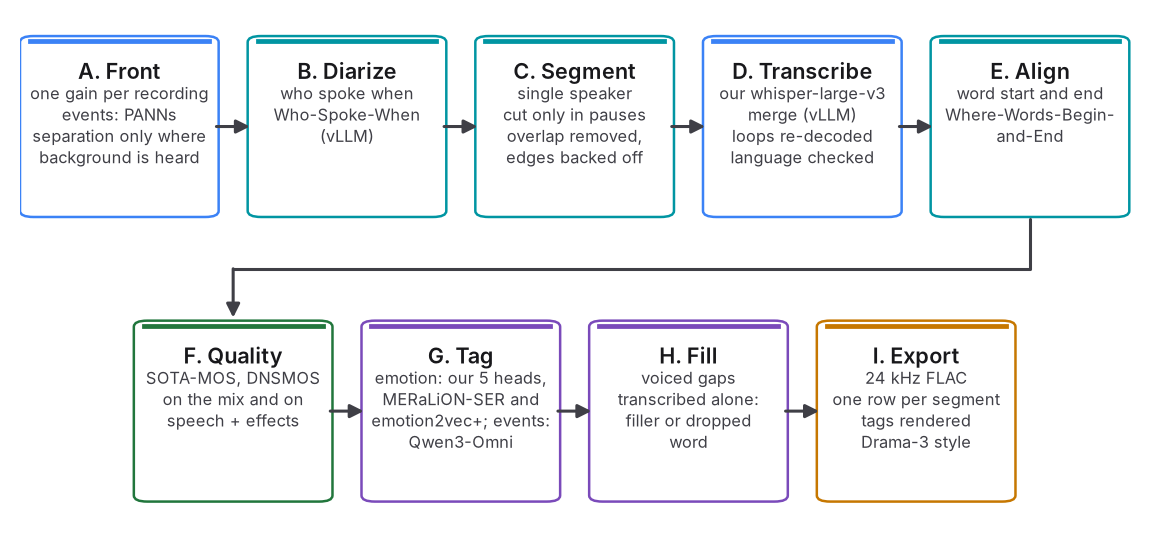
\includegraphics[width=\linewidth]{img/fig_pipeline.png}
\caption{Melati-Pipe. Nine stages, each a client of a model server (vLLM for the two Whisper-sized decoders,
dynamic-batching servers for the rest). Stage letters are used throughout the paper.}
\label{fig:pipeline}
\end{figure}

What a row of the dataset looks like, in the tag format of Fish Audio Drama 3 \citep{han2026drama3}: point tags in
square brackets act at a position, scoped tags in angle brackets act on the words they enclose, fillers stay
words.

\begin{center}
\small\texttt{<happy>hello [coughs] sorry, um, I just got the results</happy> [laughs]}
\end{center}

The tags are a rendering. The record underneath is timed: every word, filler and event has a start and an end,
and every emotion span names the words it covers, so another format is a re-rendering, not a re-annotation.

Our contributions:

\begin{itemize}
\item An audit of what Emilia-Pipe does to the audio and to the text, measured on its released Malaysian output
  and on the same recordings run through it (Section~\ref{sec:audit}).
\item A pipeline that keeps the expressive content and every model behind an API, with segmentation that cuts
  only in pauses and backs off from removed overlaps (Section~\ref{sec:pipe}).
\item A released whisper-large-v3 merge that does not hallucinate over non-speech; three defects in the training
  recipe it follows; the finding that the default decoding hid both the fix and its cost, a model that stops on
  languages it never heard; and a merge of two fine-tunes that is better than either (Section~\ref{sec:asr}).
\item Emotion heads on five frozen encoders whose average tags five emotions at measured precision where the
  released classifiers could tag three; a non-verbal classifier trained on the pipeline's own word-gap candidates,
  a gap finder that reaches the breaths it missed, and a frame-level head for the laughs and coughs over speech,
  where no gap holds them; filler tags with measured precision
  (Section~\ref{sec:tags}).
\item A released AudioSet clip tagger, distilled from the average of released ones and then of six teachers, two of them
  its own earlier versions: \val{astag/s4} mAP on the same evaluation clips where the best released one scores
  \val{astag/m/ced-base}. The six teachers' average is released too, at \val{astag/ens} (Section~\ref{sec:astagger}).
\item A side-by-side run of both pipelines on the same recordings (Section~\ref{sec:cmp}).
\end{itemize}

\section{What Emilia-Pipe does to speech}
\label{sec:audit}

Emilia-Pipe standardises a recording, separates vocals with UVR-MDX \citep{kim2021mdx}, diarizes it with
pyannote \citep{bredin2023pyannote}, cuts it with Silero VAD \citep{silero2024vad}, transcribes it with Whisper
\citep{radford2023robust} and keeps the segments DNSMOS \citep{reddy2022dnsmos} scores at 3.0 or more. We read its
code line by line (Table~\ref{tab:defects}) and measured \val{audit/v1/files} segments of each released
Malaysian-Emilia version.

\begin{table}[H]
\centering\small
\caption{Defects of upstream Emilia-Pipe, and what Melati does instead. "Fork" is the mesolitica fork that
produced Malaysian-Emilia v2. Line numbers are in the repository's \texttt{docs/emilia\_bugs.md}.}
\label{tab:defects}
\begin{tabularx}{\linewidth}{L{0.29\linewidth}L{0.12\linewidth}X}
\toprule
upstream & fork & Melati \\
\midrule
32 kbit/s MP3 export, low-passed near 8 kHz & fixed & 24 kHz FLAC \\
every segment peak-normalised to full scale & kept & one gain per recording \\
VAD only on turns over 20 s; hard 30 s cuts & kept & cuts only in pauses, within Whisper's 30 s window \\
overlapping speech kept in both speakers & kept & overlap removed from both \\
separation everywhere, vocals stem only & kept & only where background is heard; speech + effects \\
DNSMOS $\geq 3$ applied before export & kept & every score a column, none filtered on \\
language-ID confidence filters code-switching & kept & re-decode only outside the allowed languages \\
transcription prompt full of fillers & kept & a Whisper trained not to write over non-speech \\
one empty recording ends the whole run & fixed & every stage resumes from its own files \\
\bottomrule
\end{tabularx}
\end{table}

The export defect is the easiest to see. Figure~\ref{fig:ltas} is the long-term spectrum of the two releases:
v1 stops at \val{audit/v1/cutoff} kHz (its MP3s are \val{audit/v1/kbps} kbit/s, Amphion issue \#436), v2
reaches \val{audit/v2/cutoff} kHz.

\begin{figure}[H]
\centering
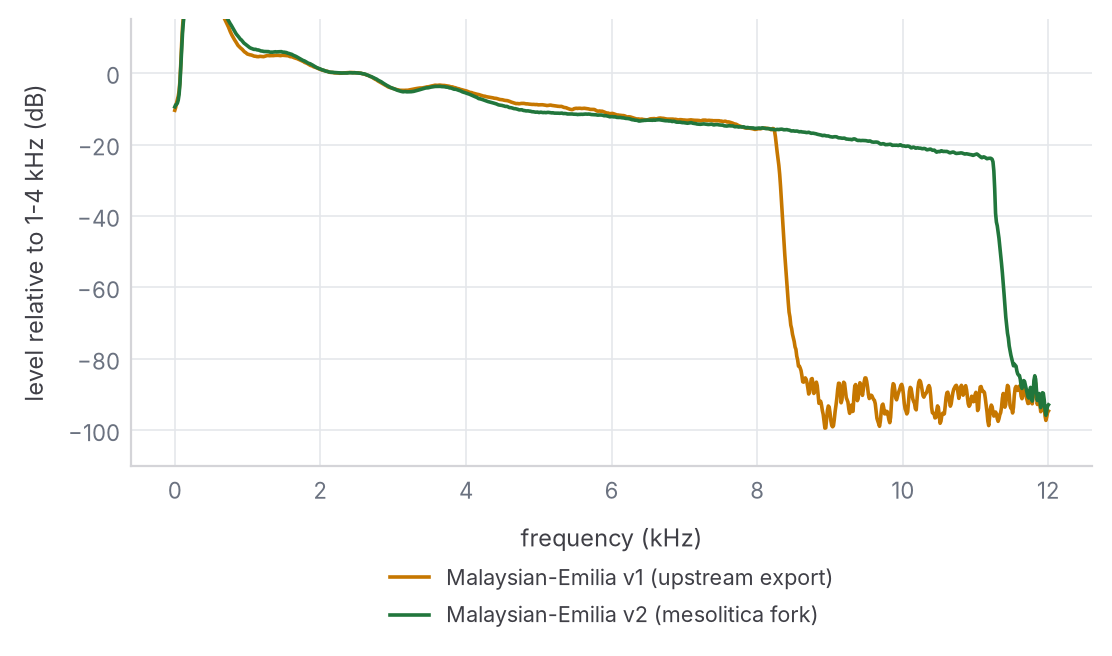
\includegraphics[width=0.86\linewidth]{img/fig_ltas.png}
\caption{Long-term average spectrum of Malaysian-Emilia v1 and v2, relative to its own 1--4 kHz level.}
\label{fig:ltas}
\end{figure}

Peak normalisation makes the level of a segment follow its loudest transient, and MP3 then pushes some over
full scale. Figure~\ref{fig:fullscale} counts the segments that touch it.

\begin{figure}[H]
\centering
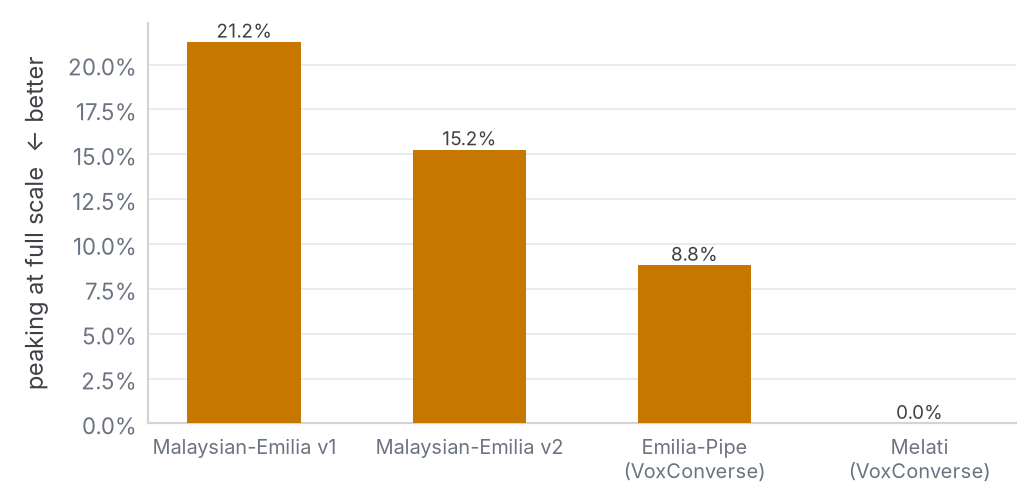
\includegraphics[width=0.78\linewidth]{img/fig_fullscale.png}
\caption{Segments whose peak is within 0.1 dB of full scale. The last two bars are the same twelve VoxConverse
recordings through each pipeline (Section~\ref{sec:cmp}).}
\label{fig:fullscale}
\end{figure}

\section{Melati-Pipe}
\label{sec:pipe}

\subsection{Every model is a server}

No pipeline code touches a GPU. Whisper and the diarization model run on vLLM \citep{kwon2023efficient}; the
separator, event detector, aligner, quality and emotion models run behind servers that batch requests as they
arrive. A recording walks the stages as a client, and many recordings are in flight at once, so while one is
being separated others are being transcribed and every server's batches stay full. Scaling is a replica count
or a tensor-parallel size in one configuration file.

\subsection{Separation that keeps the vocalisations}

Separation exists to remove music. Two things decide where Melati applies it and what it keeps. First, it runs
only where PANNs \citep{kong2020panns} hears background (music, singing, crowd, broadcast noise), because
elsewhere the recording itself is cleaner than any separator's output. Second, what it keeps: DBS-TIGER
\citep{li2025dbs,xu2025tiger}, trained on speech, music and effects \citep{petermann2022dnr}, files a laugh under
effects. We placed \val{sep/n_stimuli} real vocalisations from FSD50K \citep{fonseca2020fsd50k} in the pause
between two utterances of one Common Voice speaker \citep{ardila2020commonvoicemassivelymultilingualspeech} and
measured where each separator puts it (Figure~\ref{fig:stems}).

\begin{figure}[H]
\centering
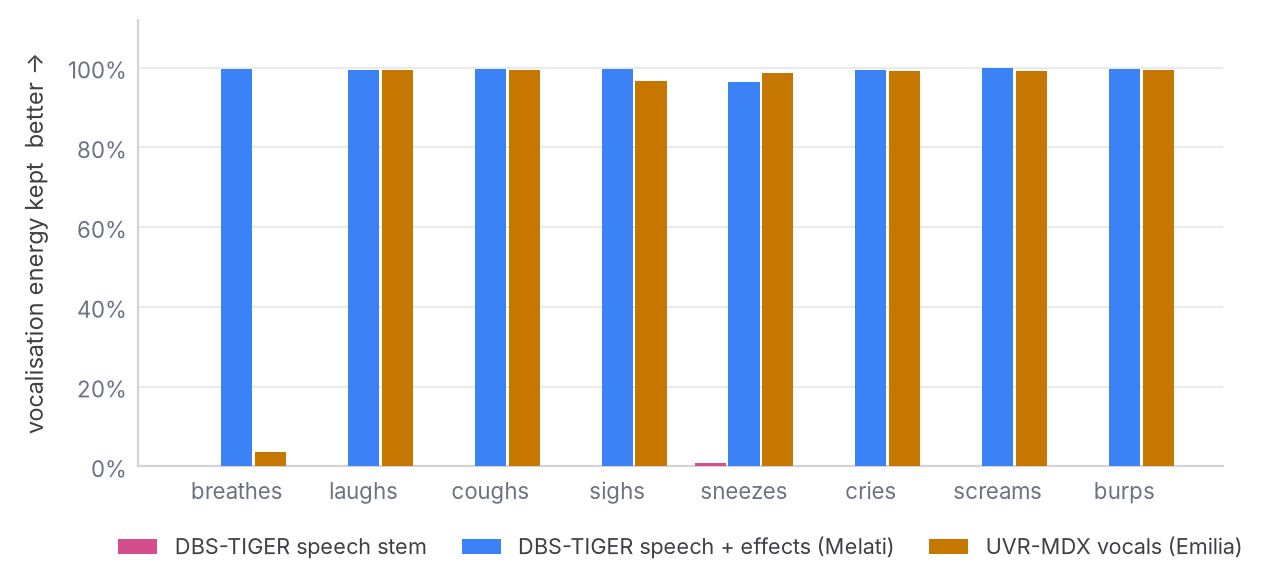
\includegraphics[width=\linewidth]{img/fig_stems.png}
\caption{Share of an injected vocalisation's energy in the stem each pipeline keeps, no music under it. The
speech stem alone keeps at most \val{sep/speech_max}; speech plus effects keeps at least \val{sep/vocal_min};
UVR-MDX keeps every class but breaths (\val{sep/uvr_breath}).}
\label{fig:stems}
\end{figure}

So Melati's separated version is speech plus effects: only the music goes. Every later stage (quality, the
taggers, export) reads that version; transcription, diarization and alignment read the speech stem, where a
laugh only gets in the way of the words.

The same stimuli show what a quality filter does to expressive speech. Adding the vocalisation lowers DNSMOS
OVRL by \val{sep/dnsmos_min} to \val{sep/dnsmos_max} and takes \val{sep/cross_min} to \val{sep/cross_max} of
otherwise clean clips under Emilia's 3.0 threshold (Figure~\ref{fig:dnsmos}). A filter applied before export
deletes segments for being expressive; Melati keeps every score as a column instead.

\begin{figure}[H]
\centering
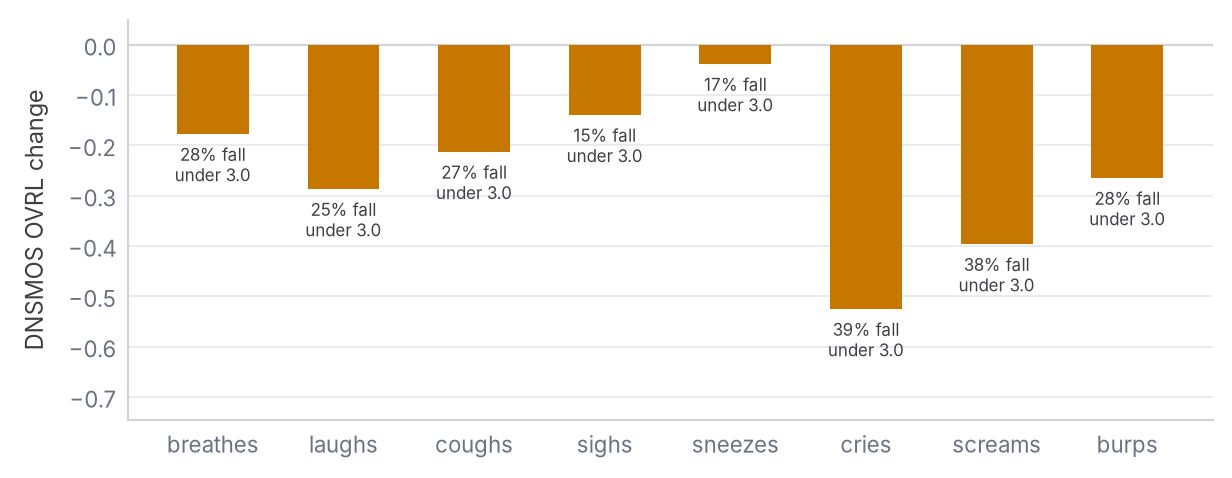
\includegraphics[width=\linewidth]{img/fig_dnsmos.png}
\caption{Change in DNSMOS OVRL when a vocalisation is added to the pause, and the share of clips it takes from
3.0 or more to under 3.0.}
\label{fig:dnsmos}
\end{figure}

\subsection{Speakers and segments}

Stage B is Who-Spoke-When \citep{khaidukova2026who}, a Whisper-based end-to-end diarizer served by vLLM; a
recording up to 45 minutes is one request (80 in the pilot; see Section~\ref{sec:v1}), a longer one is ten-minute
windows overlapping by a minute. Stage C
turns its turns into segments (Figure~\ref{fig:segment}): a cut falls only in a pause the VAD finds, a segment
never exceeds Whisper's 30-second window, and wherever two speakers overlap the overlap is removed from both, so no segment carries
a second voice. Removing an overlap cuts the first speaker off mid-word, so that edge moves back to the least
speech-like frame within 1.5 s and gets no padding. On the podcast pilot that took the segments ending inside
their last word from \val{pilb/melati_all/lastcut} to \val{pila/melati_all/lastcut}, for \val{pila/melati_all/hours}
hours exported instead of \val{pilb/melati_all/hours} (same transcriber both times).

\begin{figure}[H]
\centering
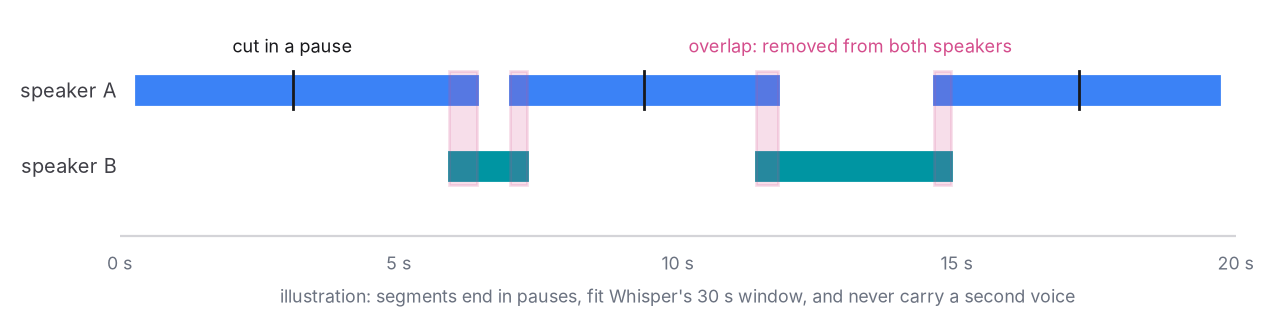
\includegraphics[width=\linewidth]{img/fig_segment.png}
\caption{Segmentation, as an illustration: cuts in pauses, overlap removed from both speakers.}
\label{fig:segment}
\end{figure}

\subsection{Words, times and quality}

Stage D is our whisper-large-v3 fine-tune (Section~\ref{sec:asr}). A segment detected outside the allowed
languages (Malay, English, Chinese, Tamil) is re-decoded with the allowed language Whisper ranks highest:
base large-v3 wrote parliamentary English as Welsh on our development set. On podcasts that re-decode lands on Tamil
for Arabic chant, songs and stray Malay, so export keeps Chinese and Tamil only where Whisper heard them itself, in a
recording mostly in that language (Section~\ref{sec:v1}). Stage E aligns the transcript with
Where-Words-Begin-and-End \citep{zolkepli2026where}, which also scores its own confidence. Stage F scores every
segment twice, on the mix and on speech plus effects, with SOTA-MOS \citep{scicom2026sotamos} and DNSMOS, and
export keeps the mix wherever the music is 25 dB under the voice and the scorer does not prefer the separated
version. Export trims a segment to 0.15 s around its first and last sound, never past the pause it was cut in.

\section{A Whisper that writes nothing over non-speech}
\label{sec:asr}

Base whisper-large-v3 writes words over \val{asr/base/silence_hr} of silent clips, \val{asr/base/music_hr} of
music and \val{asr/base/wild_words} of real voice-free audio. In a pipeline that transcribes every gap between
words to find fillers (stage H), that is a filler or a dropped word in every pause. We fine-tune it with the
recipe of \citet{zolkepli2026hallucination}: voice-free audio with empty targets, spoken hallucination phrases
with their true text, LoRA \citep{hu2022lora} rank 64 on the attention and MLP projections, 1,000 steps of 16
clips. Its paper reports a multilingual loss (FLEURS CER up for every configuration), so we add Common Voice 22
in the \val{asr/fix25/cv22_pool_langs} languages it shares with Whisper, replayed in the same batches. The mixes
are \val{asr/fix/clips} clips (no replay, \val{asr/fix/blank} voice-free) and \val{asr/fix25/clips}
(25\% replay).

\subsection{Three defects in the recipe}

The first is in what the decoder reads. The recipe masks the four prompt tokens out of the loss by setting them
to $-100$ in the labels, and lets Hugging Face build the decoder inputs from the labels. That builder shifts the
labels right and replaces every $-100$ with the pad token. So in training the decoder never sees
\tok{<|ms|><|transcribe|><|notimestamps|>}: it sees padding, and the text starts one position later than it
will at inference (Figure~\ref{fig:prefix}).

\begin{figure}[H]
\centering
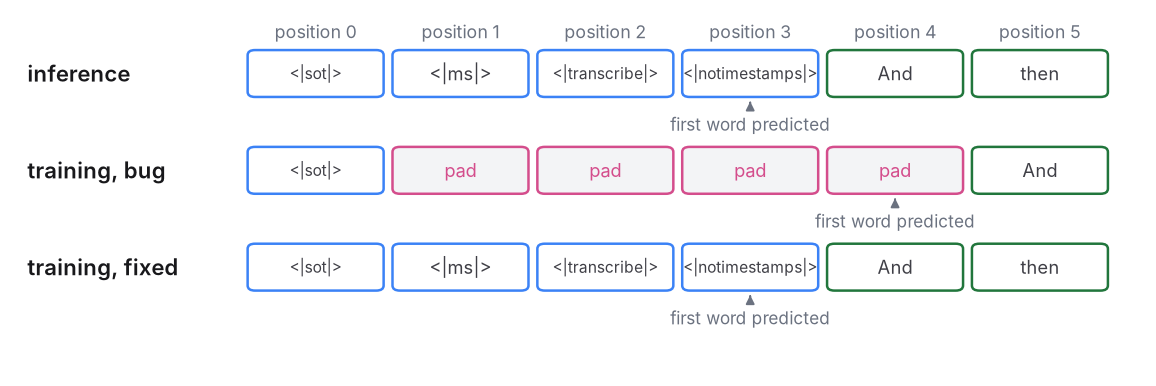
\includegraphics[width=\linewidth]{img/fig_prefix.png}
\caption{Decoder inputs for the same clip. Training with the bug never feeds the language and task tokens; the
fix feeds them as inputs and keeps them out of the loss.}
\label{fig:prefix}
\end{figure}

The second is in the full fine-tunes: the model is loaded in bfloat16 and trained in it. An AdamW step at a
learning rate of $10^{-5}$ is about 0.05\% of a typical weight, and bfloat16 resolves about 0.4\%, so most
updates round to nothing. Full fine-tunes keep fp32 master weights here (bfloat16 compute through autocast;
reentrant gradient checkpointing then has to go, because it recomputes layers against autocast's cached weight
casts).

The third is in what a checkpoint saves. Base's generation config forces \tok{<|transcribe|>}; the fine-tunes'
came out without it, so a call that names no task left the task token to the model, and a fine-tune that has
learned to obey its prompt sometimes chose \tok{<|translate|>} and wrote Yoruba as English. vLLM always states
\tok{<|transcribe|>}; so does every number below, and so does the released model's config.

\subsection{Measured as it is served}

Hugging Face's Whisper config forbids \tok{<|endoftext|>} as the first token generated after the prompt. With
the prompt stated, that is the first word, so the model cannot return an empty transcript: on a silent clip it
must write something, and a fine-tune that has learned to stop writes its second choice. vLLM, which serves the
model in the pipeline, forbids nothing. The same checkpoints decoded both ways on the
\val{asr/sup/n} voice-free clips (Figure~\ref{fig:suppress}):

\begin{figure}[H]
\centering
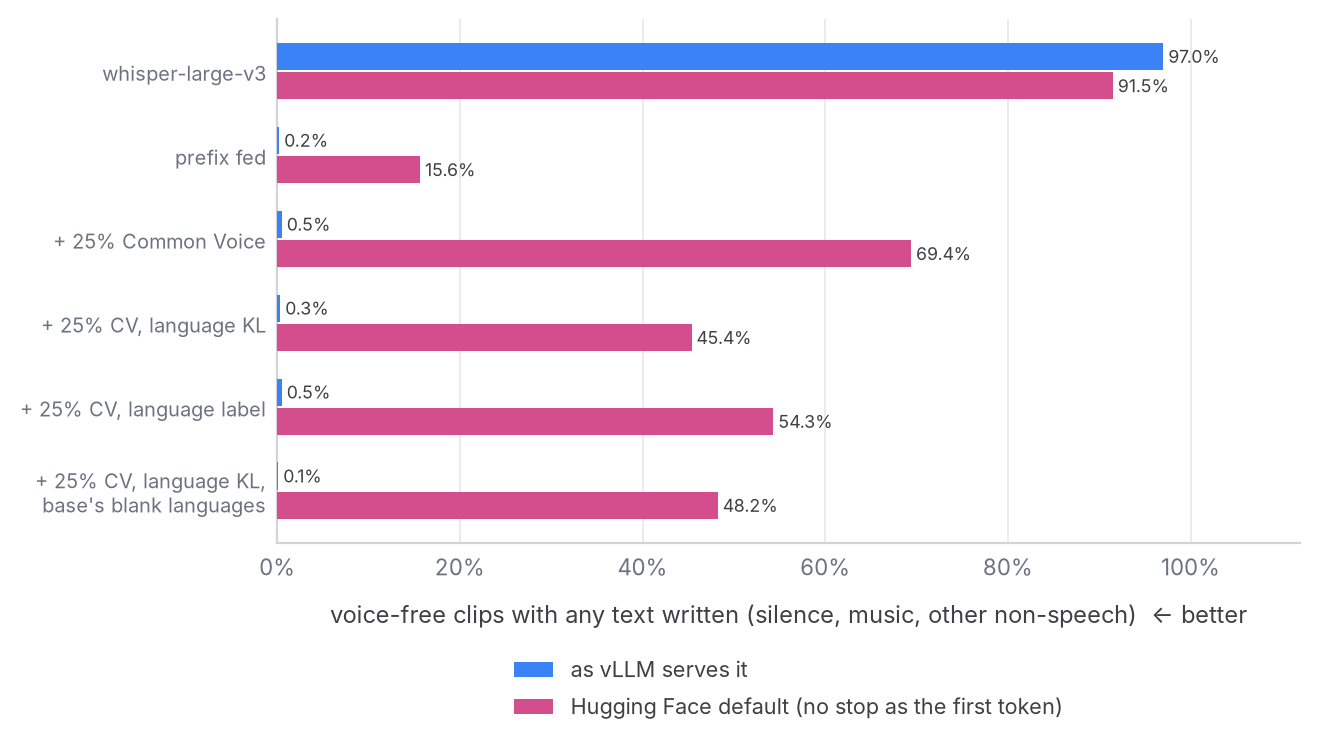
\includegraphics[width=\linewidth]{img/fig_suppress.png}
\caption{Voice-free clips (silence, music, other non-speech) with any text written, decoded with Hugging Face's
default (no stop as the first token) and as vLLM serves (nothing forbidden). Under the default the fine-tunes'
commonest outputs are a full stop, "you", "Thank you." and "Oh"; as served, nothing.}
\label{fig:suppress}
\end{figure}

Base writes over \val{asr/sup/base/hf} of them with the default and \val{asr/sup/base/vllm} as served (the
difference is music notes, which the default also suppresses): it never wanted to stop. The fine-tune with 25\%
replay writes over \val{asr/sup/fix25/hf} with the default and \val{asr/sup/fix25/vllm} as served. With the
default every clip gets some output (\val{asr/sup/fix25/hf_any}), most often a full stop or "you". Measured that
way, replay and the language losses below looked as if they gave back half of the fix; as served, none of them
did.

vLLM itself, run through its own detection and transcription prompts, wrote the same transcript as our decoding
on \val{asr/vllm/blank_same} of the \val{asr/vllm/blank_n} voice-free clips, in float16 and in bfloat16. On the
\val{asr/vllm/fleurs_n} FLEURS clips it detected the same language on \val{asr/vllm/fleurs_fp16_lang} and wrote
the same transcript on \val{asr/vllm/fleurs_fp16_same} in float16 (\val{asr/vllm/fleurs_bf16_same} in
bfloat16, which the pipeline serves); the long transcripts drift with the kernels' rounding, the error rate does
not (macro CER \val{asr/vllm/fleurs_hf_cer} ours, \val{asr/vllm/fleurs_fp16_cer} and
\val{asr/vllm/fleurs_bf16_cer} vLLM). Every number from here on is decoded as served.

\subsection{Hallucination}

As served, the fix holds (Figure~\ref{fig:halluc}). The recipe as published still writes over
\val{asr/bug/silence_hr} of silent clips and \val{asr/bug/wild_words} of real voice-free audio; fed its prefix,
the same recipe writes over \val{asr/fix/silence_hr} and \val{asr/fix/wild_words}.

\begin{figure}[H]
\centering
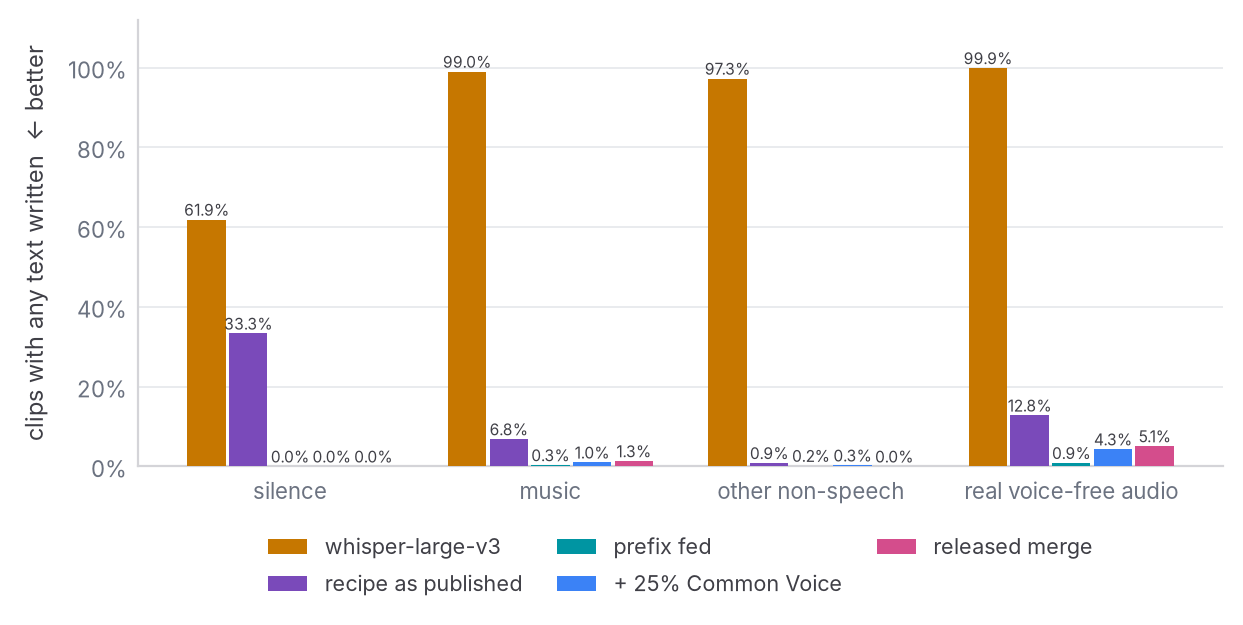
\includegraphics[width=\linewidth]{img/fig_halluc.png}
\caption{Clips with any text written, on four voice-free arms, decoded as served. "Real voice-free audio" is audio
from the wild that a VAD confirms has no voice.}
\label{fig:halluc}
\end{figure}

\subsection{What stopping costs}

A model that has learned to stop can stop on speech. Without replay it stops on whole languages
(Figure~\ref{fig:stoplangs}): fed its prefix, the fine-tune writes nothing for \val{asr/fix/fleurs_empty} of the
FLEURS clips \citep{conneau2023fleurs} (\val{asr/fleurs_clips} clips in \val{asr/fleurs_langs} languages, none
trained on), and for most of them in \val{asr/fix/fleurs_empty_top}. Its training speech was Malay, English and
the spoken hallucination phrases, so a language it never heard sounds like non-speech. With 25\% Common Voice
replayed it writes nothing for \val{asr/fix25/fleurs_empty}, and no language passes
\val{asr/fix25/fleurs_empty_max}.

\begin{figure}[H]
\centering
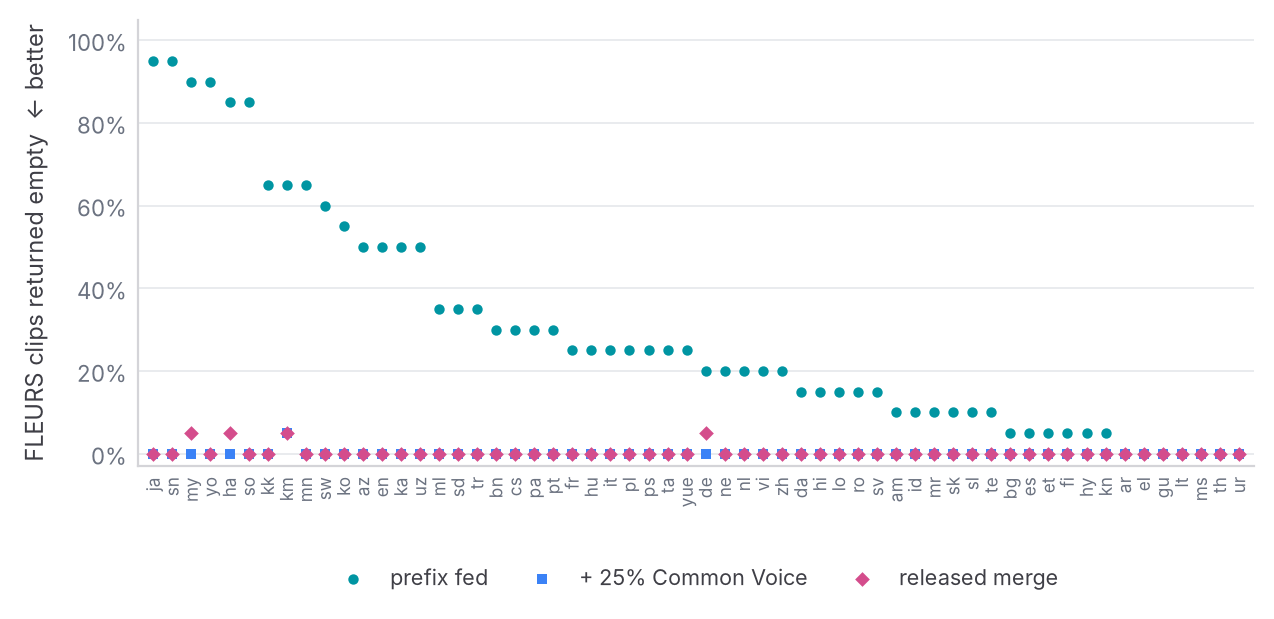
\includegraphics[width=\linewidth]{img/fig_stop_langs.png}
\caption{FLEURS clips returned empty, per language, without replay and with 25\% Common Voice replayed.}
\label{fig:stoplangs}
\end{figure}

This is the multilingual loss the recipe's paper reports, and it is larger than reported: under the default
decoding the model could not stop, so it wrote something, often the right thing.

Over every speech arm (Figure~\ref{fig:falsestop}) replay keeps the empty share near zero. One more choice raised
it. We had trained each voice-free clip under the language base detects on it, the token it meets at inference.
Base detects English on \val{asr/blank_en} of them, so the model learned to stop after \tok{<|en|>}: it returned
nothing for \val{asr/d25bl/ls_empty} of LibriSpeech, which is read English.

\begin{figure}[H]
\centering
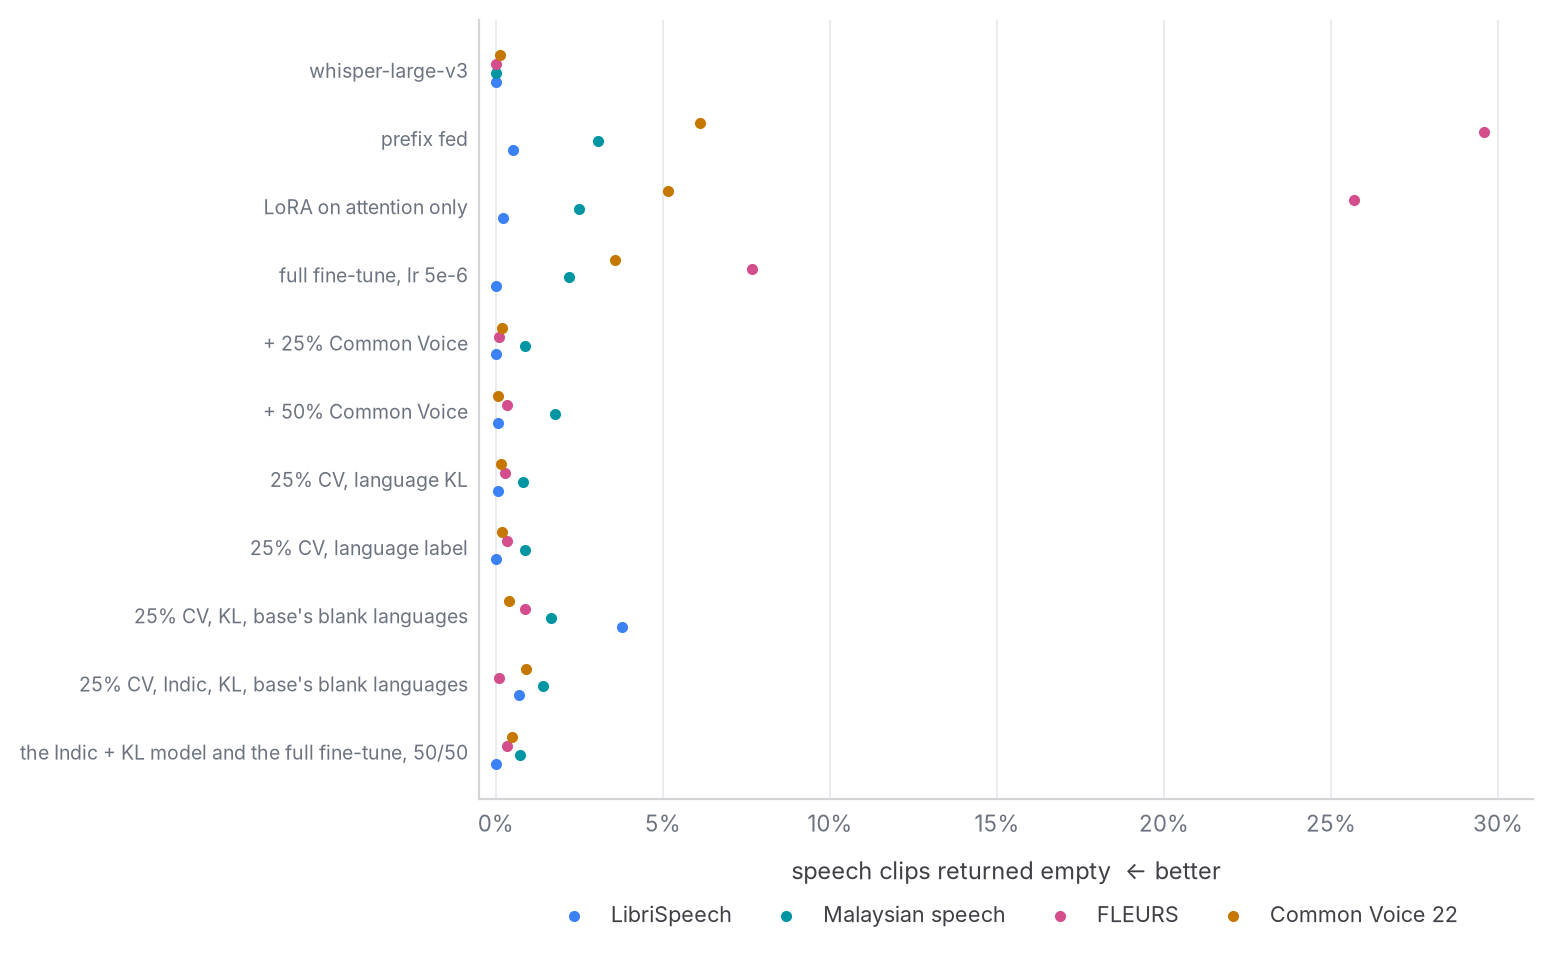
\includegraphics[width=\linewidth]{img/fig_false_stop.png}
\caption{Speech clips returned empty, per arm. Base always writes something: it cannot stop as its first token.}
\label{fig:falsestop}
\end{figure}

Noise is the other place a fine-tune stops (Figure~\ref{fig:noise}). With 25\% replay, \val{asr/fix25/noise20}
of the speech at 20 dB SNR comes back empty, and \val{asr/fix25/noisem5} at $-5$ dB.

\begin{figure}[H]
\centering
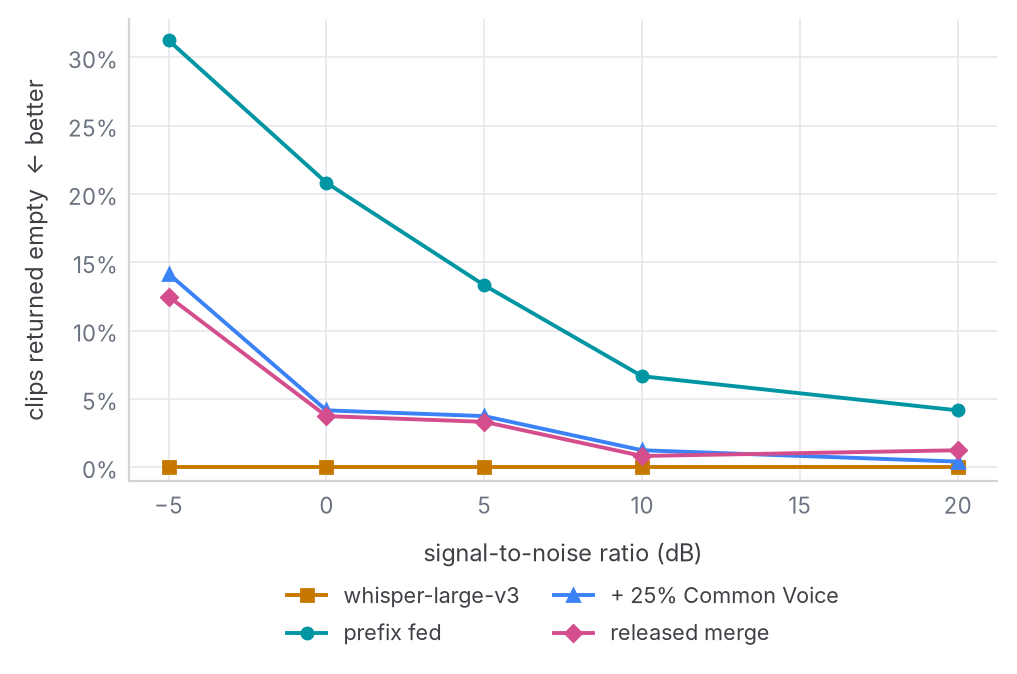
\includegraphics[width=0.78\linewidth]{img/fig_noise.png}
\caption{Speech under music or noise returned empty, by signal-to-noise ratio.}
\label{fig:noise}
\end{figure}

\subsection{The rest of the multilingual loss is language identification}

Whisper predicts the language token from the start token alone. Masked out of the loss, that prediction drifts
with every LoRA step, and a model that has learned to obey its prompt transcribes into whatever language it
guessed. Forcing each clip's language separates the two (Figure~\ref{fig:lid}): forced, the replay models
transcribe better than base (\val{asr/fix25/forced} with 25\% replay, \val{asr/base/forced} base); detected, they
are level with it (\val{asr/fix25/det}, \val{asr/base/det}).

\begin{figure}[H]
\centering
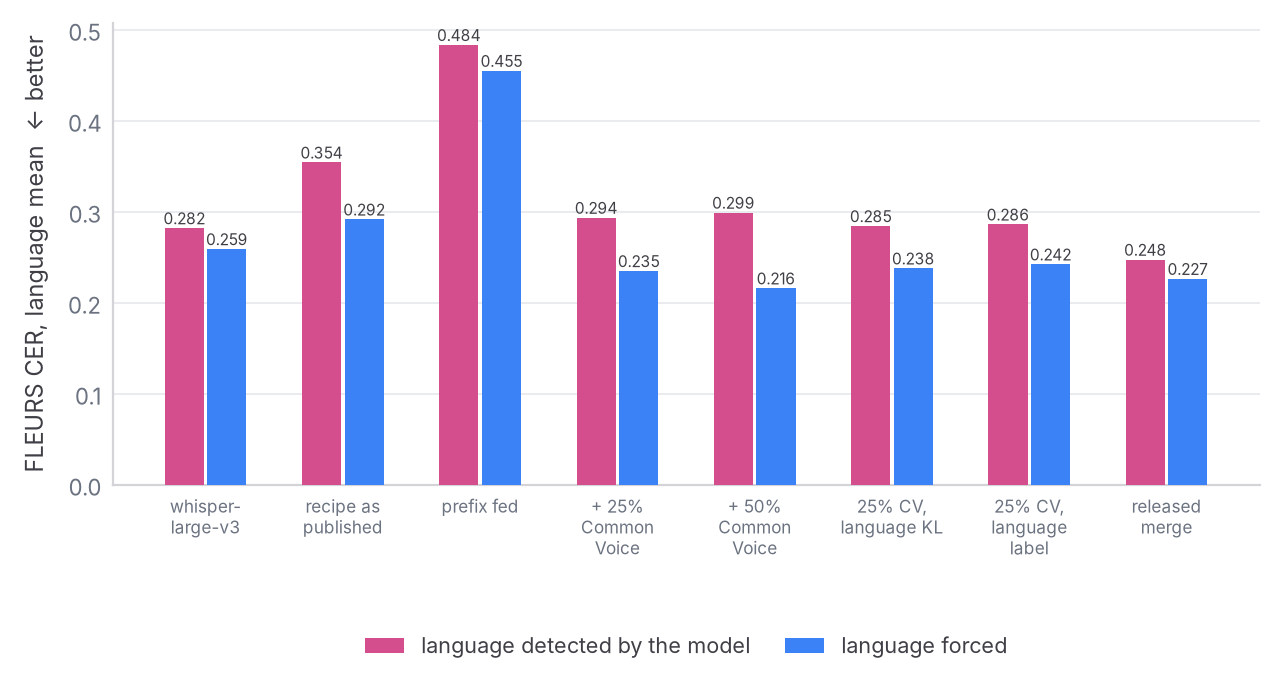
\includegraphics[width=\linewidth]{img/fig_lid.png}
\caption{FLEURS character error rate, mean over languages, with the language detected by the model and forced to
the clip's own.}
\label{fig:lid}
\end{figure}

Replay alone lowers identification, to \val{asr/fix25/lid_acc} against base's \val{asr/base/lid_acc}
(Figure~\ref{fig:lidacc}). Two losses hold it: a KL term keeping the first token's distribution over language
tokens at base's (\val{asr/distill25/lid_acc} with replay), and supervising the language token on speech
(\val{asr/label25/lid_acc}).

\begin{figure}[H]
\centering
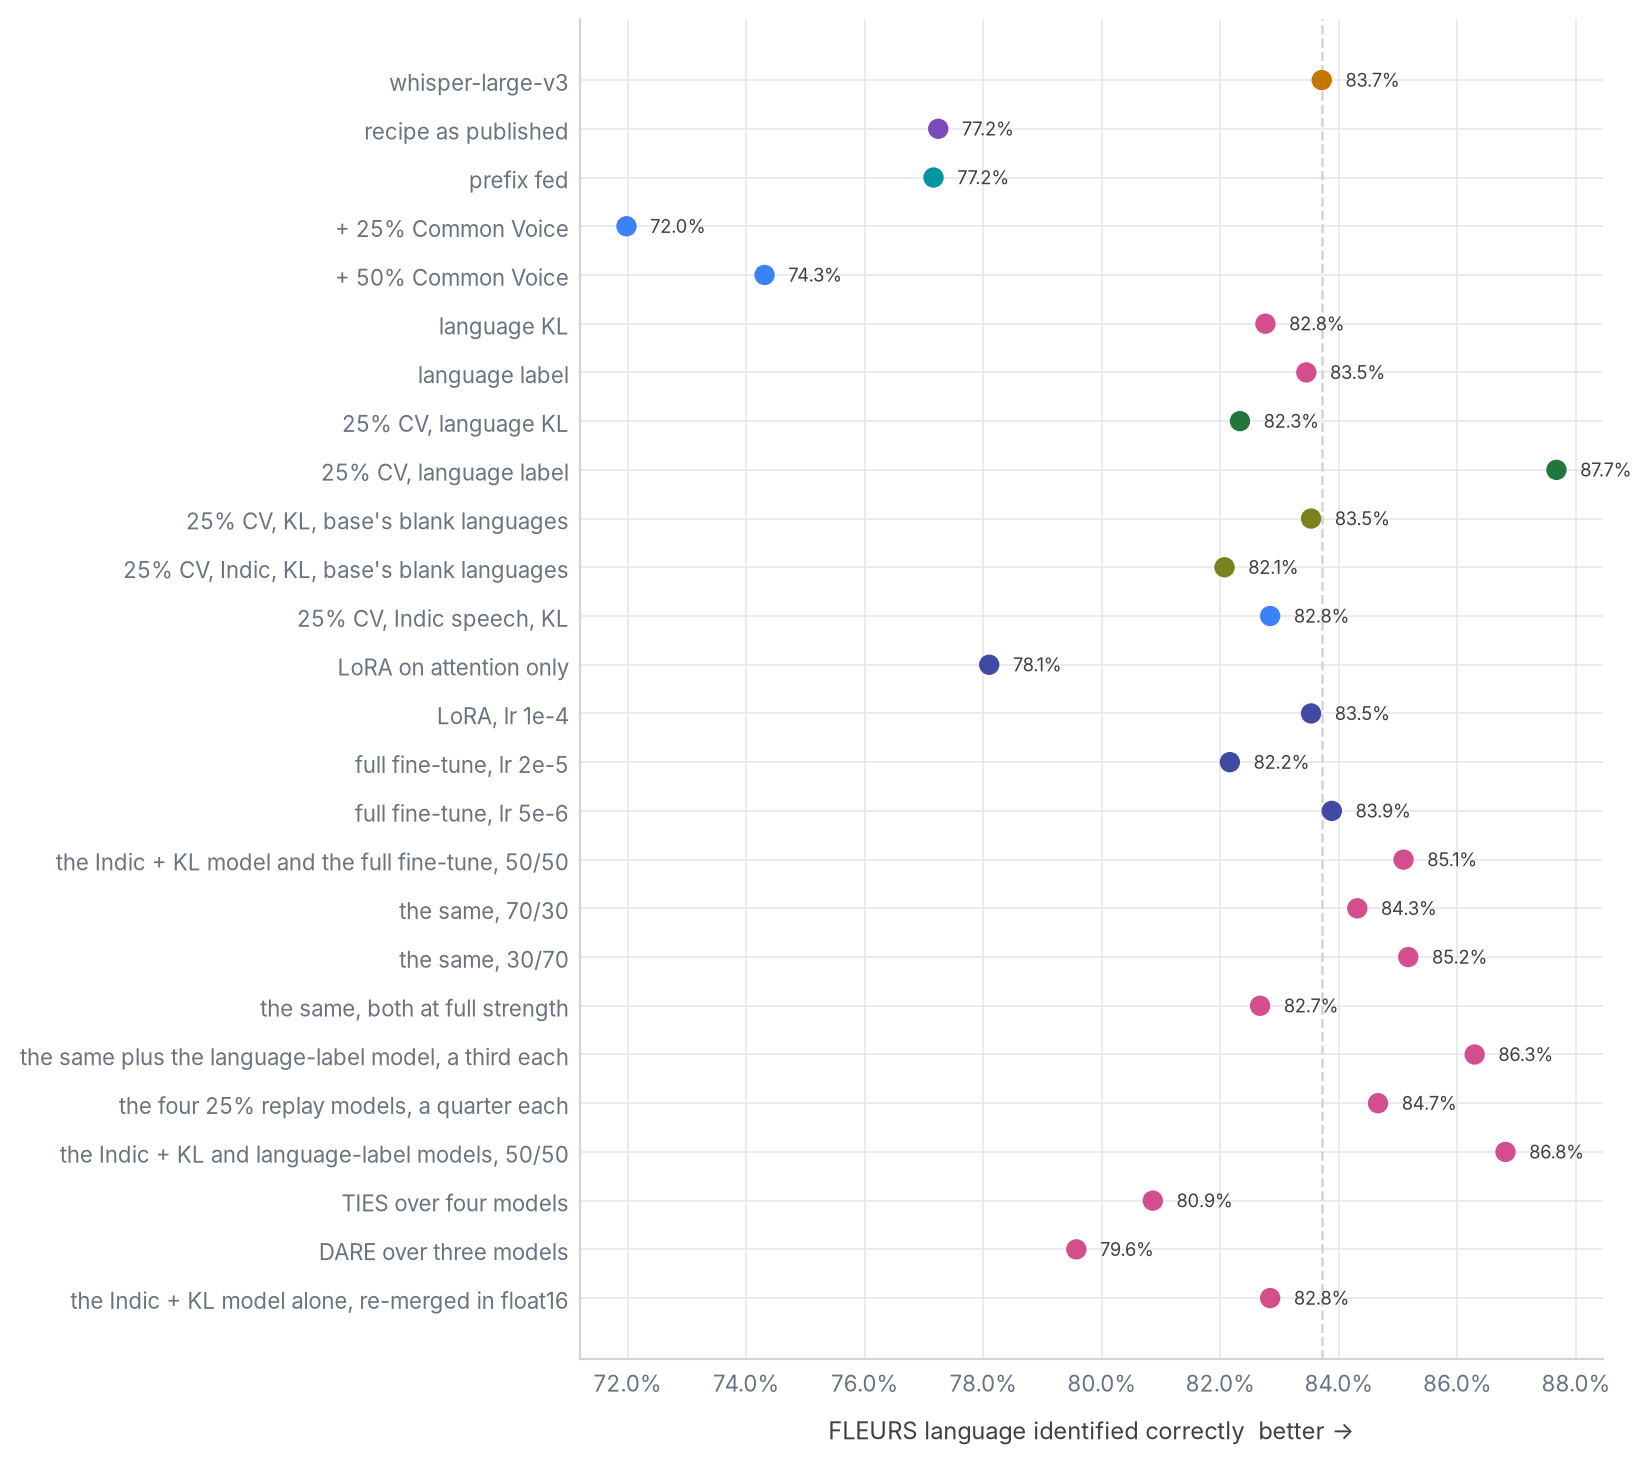
\includegraphics[width=0.86\linewidth]{img/fig_lid_acc.png}
\caption{FLEURS clips whose language the model identifies, every checkpoint. The dashed line is base.}
\label{fig:lidacc}
\end{figure}

Clips that fail outright (CER of 0.8 or more) tell the same story (Figure~\ref{fig:failed}).

\begin{figure}[H]
\centering
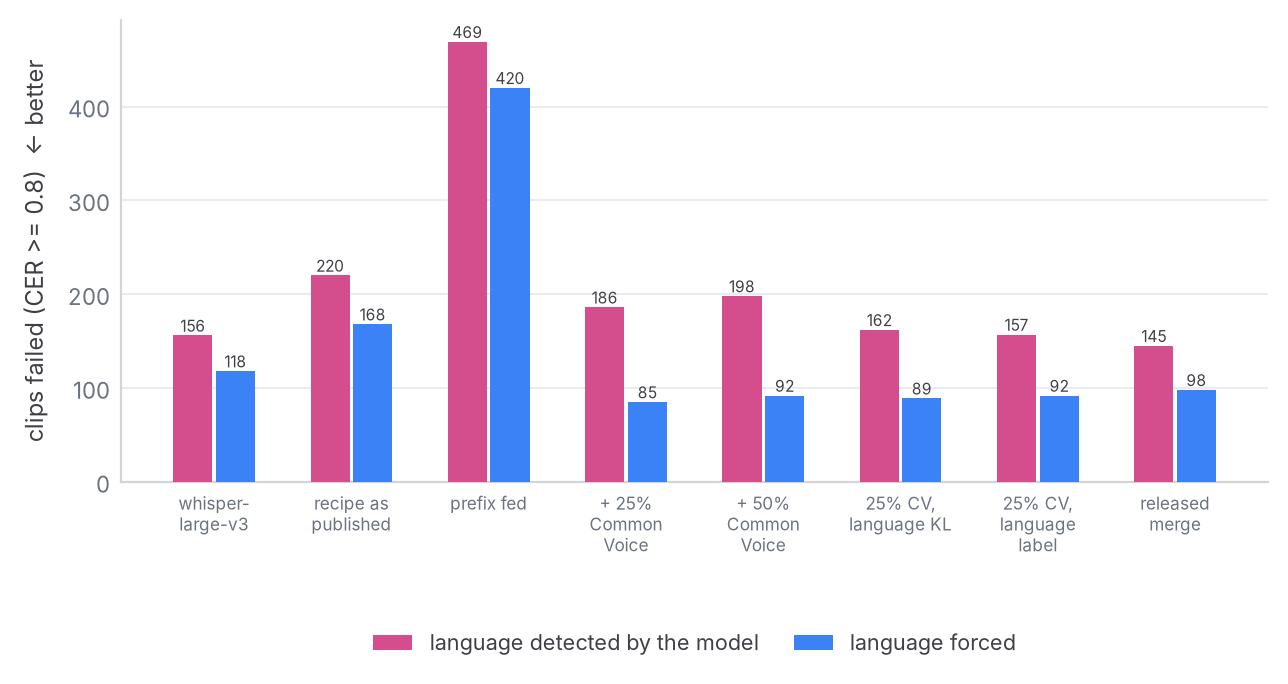
\includegraphics[width=\linewidth]{img/fig_failed.png}
\caption{FLEURS clips with a CER of 0.8 or more, out of \val{asr/fleurs_clips}.}
\label{fig:failed}
\end{figure}

\subsection{LoRA or all parameters}

The recipe's paper chose LoRA on the attention and MLP projections at $5\times10^{-4}$. On its mix, without
replay, every variant treats some languages as non-speech (Figure~\ref{fig:sweep}): the full fine-tunes least
(\val{asr/full5e-6/fleurs_empty} of FLEURS at $5\times10^{-6}$), LoRA on attention only nearly as much as the
recipe. Replay matters more than the method.

\begin{figure}[H]
\centering
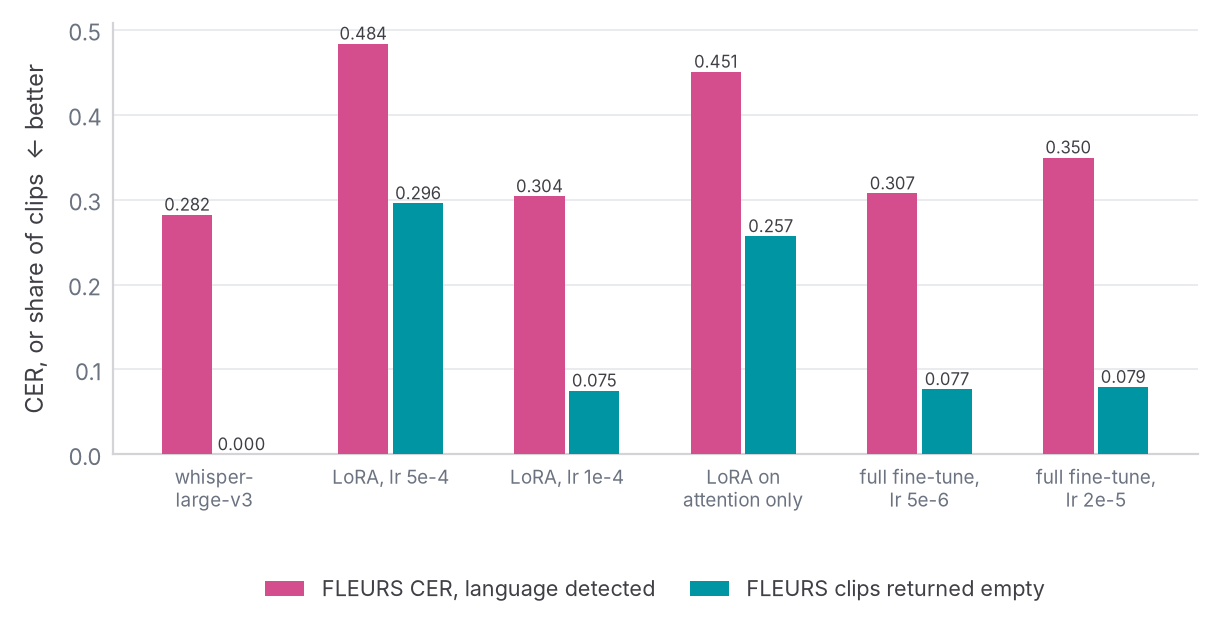
\includegraphics[width=\linewidth]{img/fig_sweep.png}
\caption{The same mix, no replay, five ways of training: FLEURS CER with the language detected, and the share of
FLEURS clips returned empty.}
\label{fig:sweep}
\end{figure}

\subsection{Loops}

Asked to transcribe a syllable said several times, the replay fine-tunes sometimes cannot stop
(Figure~\ref{fig:runaway}): for "ta" said eight times, the model with 25\% replay and the language KL wrote "ta"
until its 440-token limit. The loops were there before the decoding changed. Melati's ASR stage guards against them
the way Whisper's own decoder does: a transcript that compresses like a loop (gzip ratio over 2.4) is decoded
again at temperatures 0.2, 0.4 and 0.6, and every decode is capped at 15 tokens per second of audio.

\begin{figure}[H]
\centering
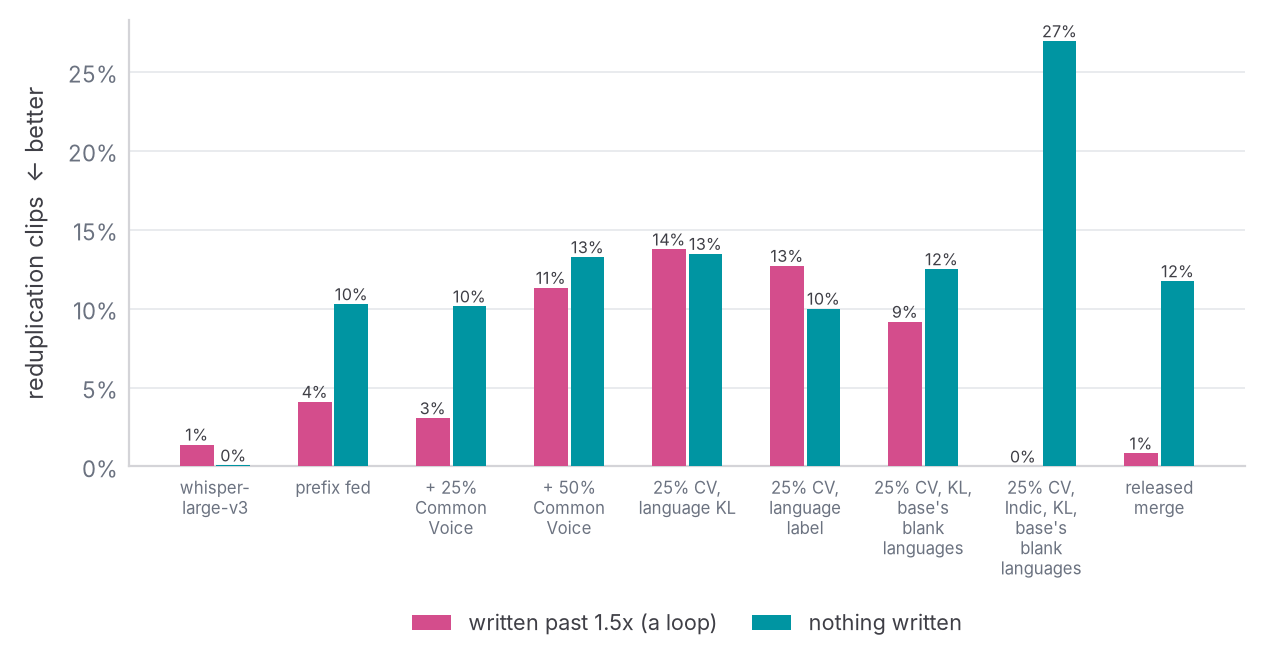
\includegraphics[width=\linewidth]{img/fig_runaway.png}
\caption{The reduplication arm (a syllable said $n$ times): clips where it is written more than $1.5n$ times, and
clips where nothing is written.}
\label{fig:runaway}
\end{figure}

\subsection{Merging}

Each fine-tune did one thing well. Replay with the Indic arm and the language KL kept the languages; the full
fine-tune at $5\times10^{-6}$ barely loops and has the best LibriSpeech WER; supervising the language token held
identification best. All are changes to the same base, so they can be added \citep{wortsman2022soups,ilharco2023task}.
We rebuilt every LoRA change exactly from its fp32 adapter (the merged checkpoints were saved in bfloat16;
re-merging the Indic + KL model alone in float16 gave the same numbers), averaged the changes with weights, and
scored each merge on the arms that separate the fine-tunes (Table~\ref{tab:merge}).

\begin{table}[H]
\centering
\footnotesize
\begin{tabular}{lrrrrrr}
\toprule
 & loops & LibriSp. & Malaysian & FLEURS & FL. empty & lang. ID \\
\midrule
whisper-large-v3 & \val{asr/base/runaway} & \val{asr/base/librispeech_wer} & \val{asr/base/genuine_wer} & \val{asr/base/det} & \val{asr/base/fleurs_empty} & \val{asr/base/lid_acc} \\
Indic + KL & \val{asr/tts/runaway} & \val{asr/tts/librispeech_wer} & \val{asr/tts/genuine_wer} & \val{asr/tts/det} & \val{asr/tts/fleurs_empty} & \val{asr/tts/lid_acc} \\
full fine-tune, $5\times10^{-6}$ & \val{asr/full5e-6/runaway} & \val{asr/full5e-6/librispeech_wer} & \val{asr/full5e-6/genuine_wer} & \val{asr/full5e-6/det} & \val{asr/full5e-6/fleurs_empty} & \val{asr/full5e-6/lid_acc} \\
\midrule
the two, 50/50 (released) & \val{asr/merge/runaway} & \val{asr/merge/librispeech_wer} & \val{asr/merge/genuine_wer} & \val{asr/merge/det} & \val{asr/merge/fleurs_empty} & \val{asr/merge/lid_acc} \\
the two, 70/30 & \val{asr/m_7030/runaway} & \val{asr/m_7030/librispeech_wer} & \val{asr/m_7030/genuine_wer} & \val{asr/m_7030/det} & \val{asr/m_7030/fleurs_empty} & \val{asr/m_7030/lid_acc} \\
the two, 30/70 & \val{asr/m_3070/runaway} & \val{asr/m_3070/librispeech_wer} & \val{asr/m_3070/genuine_wer} & \val{asr/m_3070/det} & \val{asr/m_3070/fleurs_empty} & \val{asr/m_3070/lid_acc} \\
the two, both at full strength & \val{asr/m_sum/runaway} & \val{asr/m_sum/librispeech_wer} & \val{asr/m_sum/genuine_wer} & \val{asr/m_sum/det} & \val{asr/m_sum/fleurs_empty} & \val{asr/m_sum/lid_acc} \\
the two + label model, a third each & \val{asr/m_three/runaway} & \val{asr/m_three/librispeech_wer} & \val{asr/m_three/genuine_wer} & \val{asr/m_three/det} & \val{asr/m_three/fleurs_empty} & \val{asr/m_three/lid_acc} \\
four replay models, a quarter each & \val{asr/m_soup/runaway} & \val{asr/m_soup/librispeech_wer} & \val{asr/m_soup/genuine_wer} & \val{asr/m_soup/det} & \val{asr/m_soup/fleurs_empty} & \val{asr/m_soup/lid_acc} \\
TIES, four models & \val{asr/m_ties/runaway} & \val{asr/m_ties/librispeech_wer} & \val{asr/m_ties/genuine_wer} & \val{asr/m_ties/det} & \val{asr/m_ties/fleurs_empty} & \val{asr/m_ties/lid_acc} \\
DARE, three models & \val{asr/m_dare/runaway} & \val{asr/m_dare/librispeech_wer} & \val{asr/m_dare/genuine_wer} & \val{asr/m_dare/det} & \val{asr/m_dare/fleurs_empty} & \val{asr/m_dare/lid_acc} \\
\bottomrule
\end{tabular}
\caption{Merges of the fine-tunes' weight changes, decoded as served. Loops: reduplication clips written past
1.5$\times$. WER is over every reference word; FLEURS is CER with the language detected.}
\label{tab:merge}
\end{table}

Averaging the Indic + KL model with the full fine-tune, half each, beat both on Malaysian speech and FLEURS, kept
language identification above base and cut the loops to \val{asr/merge/runaway}. Shifting the weights trades loops
against FLEURS clips returned empty; adding both changes at full strength, TIES \citep{yadav2023ties} and DARE
\citep{yu2024dare} were worse, and averaging the four replay models brought the loops back.

\subsection{The released model}

The released model is that half-and-half merge, at
\url{https://huggingface.co/Scicom-intl/Melati-Whisper-Large-V3} (Table~\ref{tab:release}). Its generation config
suppresses nothing and states the transcribe task, so \texttt{transformers} decodes it as vLLM does.

\begin{table}[H]
\centering
\small
\begin{tabular}{lrr}
\toprule
 & whisper-large-v3 & released \\
\midrule
Silence, music, other non-speech with text & \val{asr/base/silence_hr}, \val{asr/base/music_hr}, \val{asr/base/nonspeech_hr} & \val{asr/merge/silence_hr}, \val{asr/merge/music_hr}, \val{asr/merge/nonspeech_hr} \\
Real voice-free audio with text & \val{asr/base/wild_words} & \val{asr/merge/wild_words} \\
Spoken hallucination phrases transcribed & \val{asr/base/lexicon_recovered} & \val{asr/merge/lexicon_recovered} \\
FLEURS CER, language detected / forced & \val{asr/base/det} / \val{asr/base/forced} & \val{asr/merge/det} / \val{asr/merge/forced} \\
FLEURS language identified & \val{asr/base/lid_acc} & \val{asr/merge/lid_acc} \\
Common Voice 22 CER & \val{asr/base/cv22} & \val{asr/merge/cv22} \\
LibriSpeech test-clean WER & \val{asr/base/librispeech_wer} & \val{asr/merge/librispeech_wer} \\
Malaysian speech WER & \val{asr/base/genuine_wer} & \val{asr/merge/genuine_wer} \\
Returned empty: LibriSpeech, Malaysian, FLEURS & \val{asr/base/ls_empty}, \val{asr/base/my_empty}, \val{asr/base/fleurs_empty} & \val{asr/merge/ls_empty}, \val{asr/merge/my_empty}, \val{asr/merge/fleurs_empty} \\
Reduplication: loops, nothing written & \val{asr/base/runaway}, \val{asr/base/redup_empty} & \val{asr/merge/runaway}, \val{asr/merge/redup_empty} \\
\bottomrule
\end{tabular}
\caption{The released model against base, decoded as served. WER is over every reference word.}
\label{tab:release}
\end{table}

Language by language (Figure~\ref{fig:perlang}) it sits on or under base for most of FLEURS.

\begin{figure}[H]
\centering
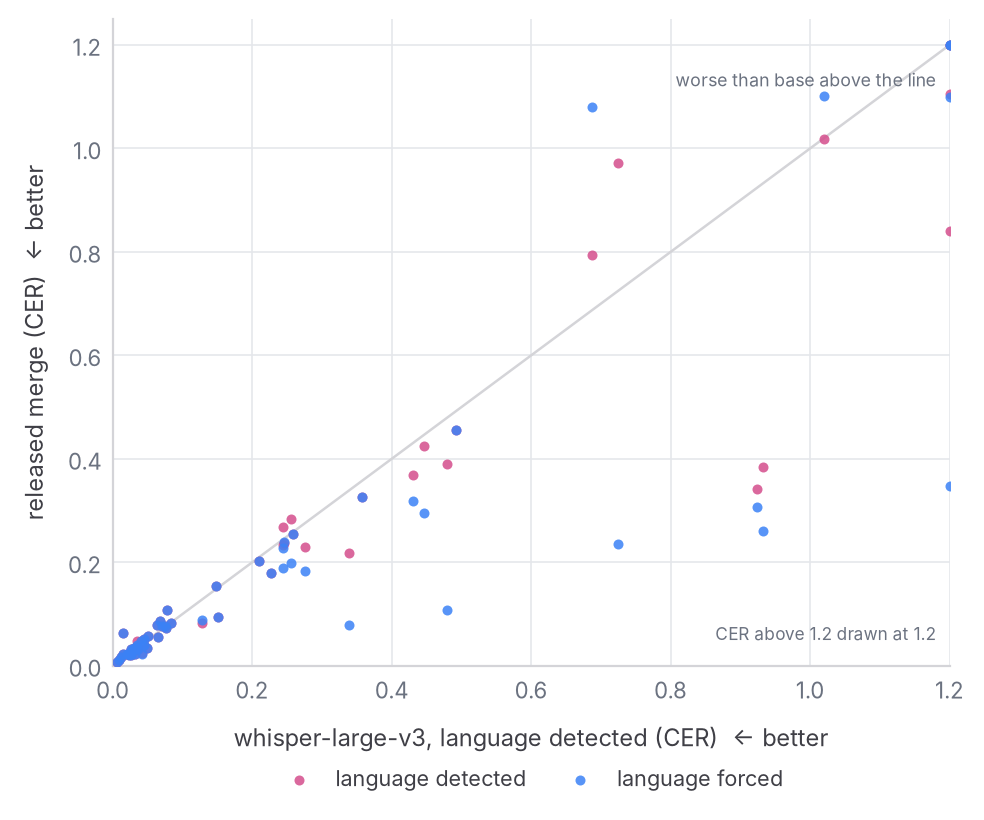
\includegraphics[width=0.74\linewidth]{img/fig_perlang.png}
\caption{FLEURS CER per language, base (x) against the released merge (y), with the language detected and forced.}
\label{fig:perlang}
\end{figure}

\section{Tags with measured precision}
\label{sec:tags}

A tag in a training transcript is an instruction to a speech generator, so a wrong tag is worse than a missing
one. Every tag class here is kept only where its precision was measured on held-out labels, and the threshold
is the one that measurement chose.

\subsection{Emotion}

We started from two released classifiers: MERaLiON-SER \citep{sailor2025meralionser}, trained for English,
Chinese, Malay and Tamil, and emotion2vec+ large \citep{ma2023emotion2vec}. emotion2vec+ was fine-tuned on EmoBox
\citep{ma2024emobox}, whose 32 corpora include \val{emo/seen} of CAMEO's thirteen \citep{christop2025cameo}, and on
those it is near perfect (Figure~\ref{fig:emocorpus}). Only corpora outside every model's training data say
anything: nEMO \citep{christop2024nemo} (Polish, acted) and the VoxCeleb half of NonverbalTTS
\citep{borisov2025nonverbaltts} (English interviews), \val{emo2/held_clips} clips.

\begin{figure}[H]
\centering
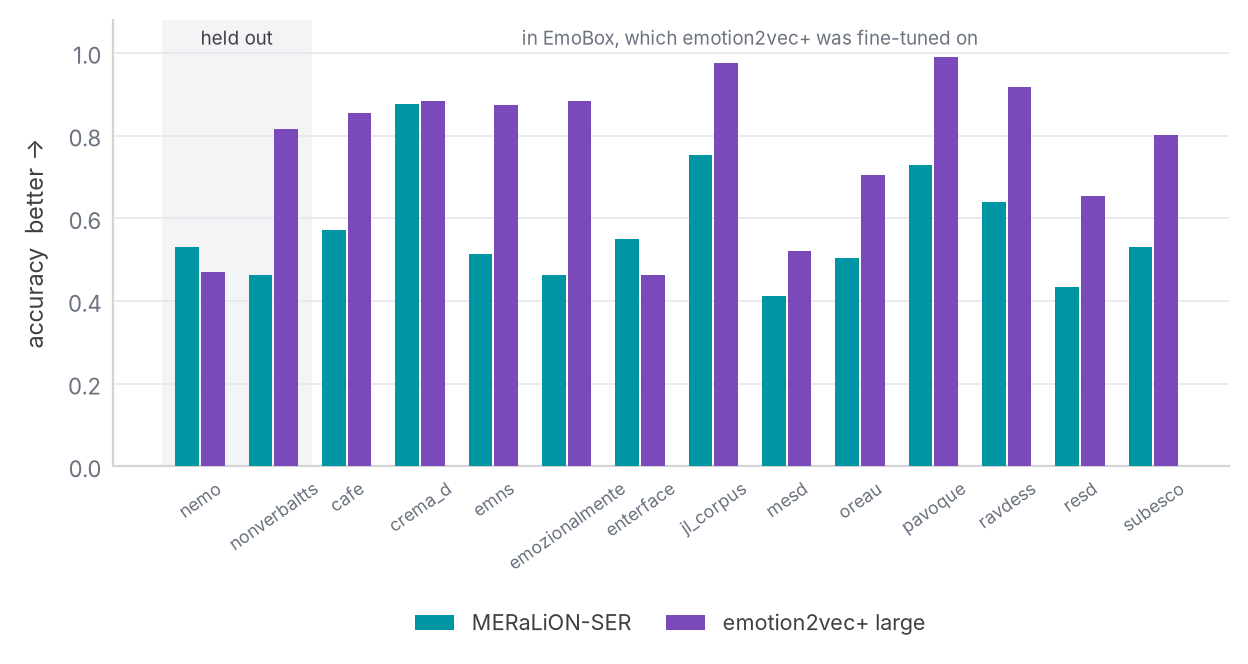
\includegraphics[width=\linewidth]{img/fig_emo_corpus.png}
\caption{Accuracy per corpus. The shaded corpora are held out from every model we know the training data of.}
\label{fig:emocorpus}
\end{figure}

\paragraph{Our own heads.} We trained a small head (a learned mix of the encoder's layers, mean-pooled over the
clip, then one hidden layer) on five frozen encoders: Whisper-large-v3 \citep{radford2023robust}, the strongest
backbone in EmoBox's benchmark; Melati's own Whisper fine-tune; w2v-BERT 2.0 \citep{seamless2023}; WavLM-large
\citep{chen2022wavlm}; and emotion2vec+'s features. The training set
is every corpus of EmoBox we could download without a signed agreement, CAMEO, Expresso and the Expresso half of
NonverbalTTS: \val{emo2/train_clips} clips from \val{emo2/train_corpora} corpora in \val{emo2/train_langs}
languages, with every corpus weighted equally in the loss. It includes \val{emo2/meld_n} clips of MELD
\citep{poria2019meld}, TV dialogue, the nearest thing to conversation that is openly licensed. On the held-out
clips the head on Whisper-large-v3 beats both released classifiers alone and averaged
(Figure~\ref{fig:emoheads}); averaging all seven models does better still, \val{emo2/ens/uar} against
\val{emo2/cur/uar}.

\begin{figure}[H]
\centering
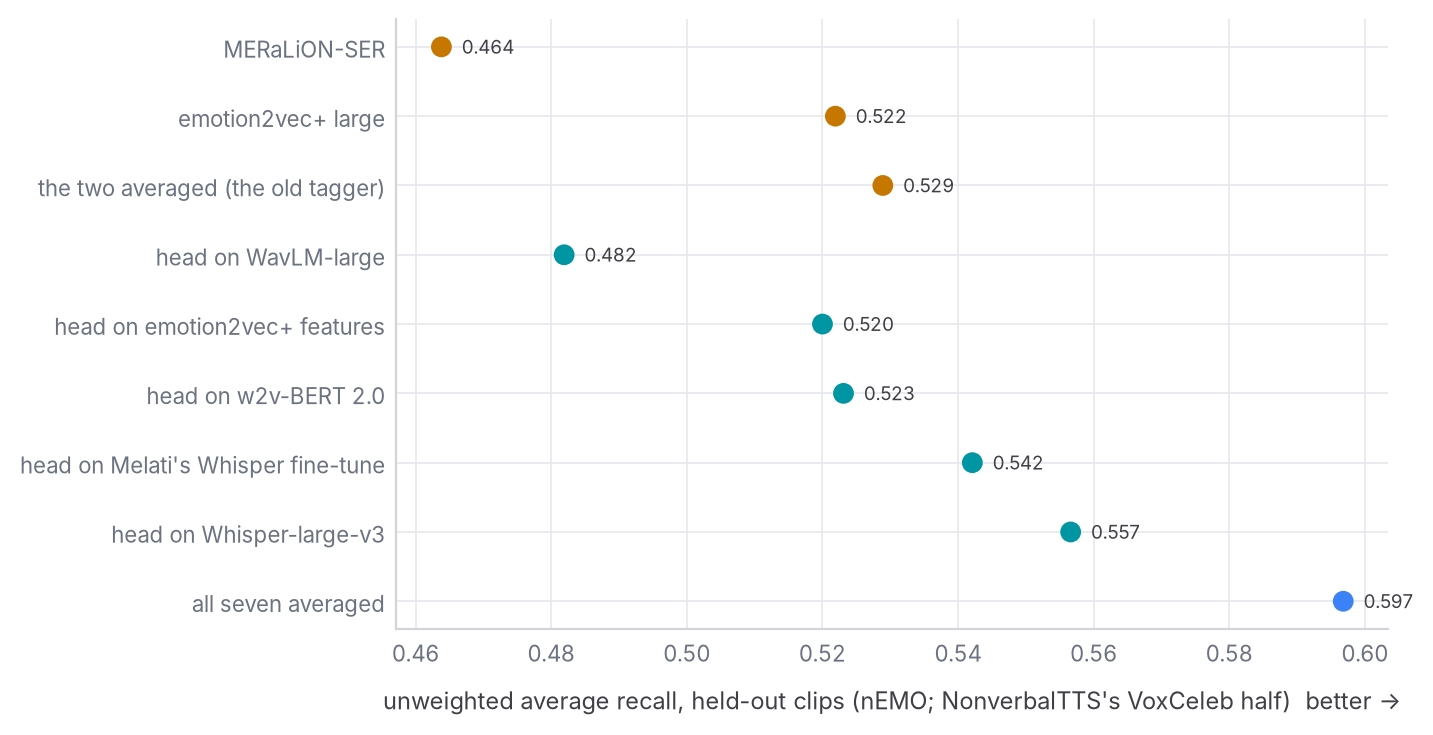
\includegraphics[width=0.86\linewidth]{img/fig_emo_heads.png}
\caption{Unweighted average recall on the \val{emo2/held_clips} held-out clips, every model scored on the same
clips. The seven are averaged as they are, not picked after the fact.}
\label{fig:emoheads}
\end{figure}

\paragraph{When a label is tagged.} Acted corpora are balanced; podcasts are mostly neutral. A threshold with 0.8
precision when a seventh of the clips are angry has far less when one in twenty is. So precision is re-weighted
to an assumed podcast rate per label (happy \val{emo/prior/happy}, sad, angry and surprised
\val{emo/prior/angry}, fearful and disgusted \val{emo/prior/fearful}), and a label is tagged only where that
precision reaches \val{emo/target}. The threshold is chosen on one half of the held-out clips and its recall
measured on the other (Figure~\ref{fig:emorecall}). The old tagger could tag happy, angry and surprised; the seven
together also tag sad (\val{emo2/ens/sad/recall}) and fearful (\val{emo2/ens/fearful/recall}), and find more of
the happy clips (\val{emo2/ens/happy/recall} against \val{emo2/cur/happy/recall}). Disgust has no held-out
examples and is never tagged. Every label's probability stays in the dataset.

\begin{figure}[H]
\centering
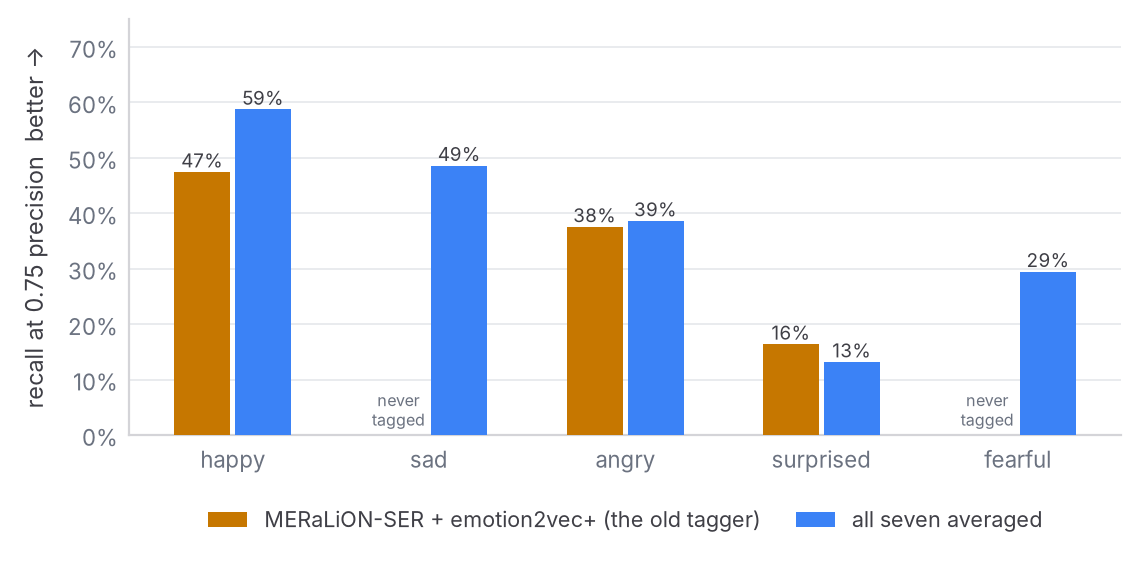
\includegraphics[width=\linewidth]{img/fig_emo_recall.png}
\caption{Recall at 0.75 precision, re-weighted to podcast rates, held-out clips; the threshold is chosen on one
half and measured on the other.}
\label{fig:emorecall}
\end{figure}

\paragraph{Mandarin film and TV.} MER2023 \citep{lian2023mer}, licensed for academic research, adds
\val{emo3/mer/n} labelled clips of Mandarin film and television, "worried" folded into fearful as anxiety is.
Left out of training, the head on Whisper-large-v3 scores \val{emo3/mer/loco/whisper} UAR on it (emotion2vec+'s
features, which saw it during their own training, \val{emo3/mer/loco/e2v}) and hears \val{emo3/mer/fear/whisper}
of the worried clips as fearful. Trained in, it moves the held-out average by less than one seed would
(Figure~\ref{fig:emomer}): \val{emo3/ens/uar} against \val{emo2/ens/uar}, nEMO \val{emo3/nemo} against
\val{emo2c/nemo}, NonverbalTTS \val{emo3/nvtts} against \val{emo2c/nvtts}. The tagger stays as it was.

\begin{figure}[H]
\centering
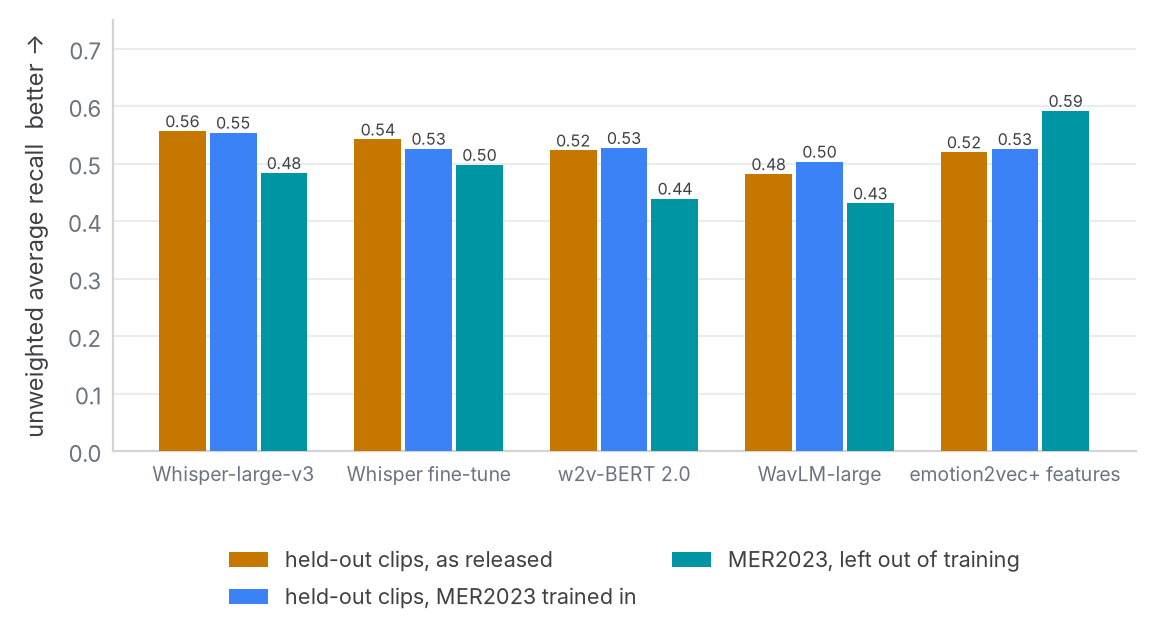
\includegraphics[width=0.92\linewidth]{img/fig_emo_mer.png}
\caption{Each head on the held-out clips, as released and with MER2023 trained in, and on MER2023 when it is
left out of training.}
\label{fig:emomer}
\end{figure}

None of these held-out clips is Malaysian. \val{emo/my_sample} segments of the podcast pilot, \val{emo/my_random}
of them drawn at random to measure how often each emotion really occurs, are ready for native speakers to label
on a page that keeps the audio on our server; until they are, the precision on Malaysian podcasts is assumed.

\subsection{Non-verbal sounds}

NonverbalTTS marks vocalisations inline, at the word boundary where they happen; its test split has
\val{nv/ref/breath} breaths, \val{nv/ref/laugh} laughs and \val{nv/ref/cough} coughs in \val{nv/test_clips}
clips. A tag counts when it lands within one word of a reference tag of its class. We tried three ways.

An audio event detector, PANNs, placed at the nearest word boundary: precise and nearly blind
(laughs \val{nv/panns/laugh/p} precision, \val{nv/panns/laugh/r} recall; breaths \val{nv/panns/breath/r} recall).
An audio language model asked to transcribe and tag in one pass: Qwen3-Omni finds more, and its wording decides
how much (with a prompt that asks for every breath, breath recall rises to \val{nv/omnis/breath/r}), but its tags
land at the wrong word (\val{nv/omnis/breath/place} of its breath tags within one word) and it invents throat
clearing (\val{nv/omnis/throat_clear/fp} clips with none).

So we split the question (Figure~\ref{fig:gapmethod}). Where: the aligned words leave gaps, and a gap with sound
above both the clip's noise floor and a level 40 dB under its speech is a candidate, with its own times. What:
each candidate, cut out and padded with silence, goes to Qwen3-Omni with a closed list of sixteen labels as
letters (speech, filler, breath, laugh, cough, sigh and so on, silence and noise included), and the probability
of each letter is read from the first answer token. A class is tagged where its probability clears a threshold
chosen on \val{nv/calib_clips} NonverbalTTS training clips for \val{nv/target} precision; the test split takes no
part in that choice.

\begin{figure}[H]
\centering
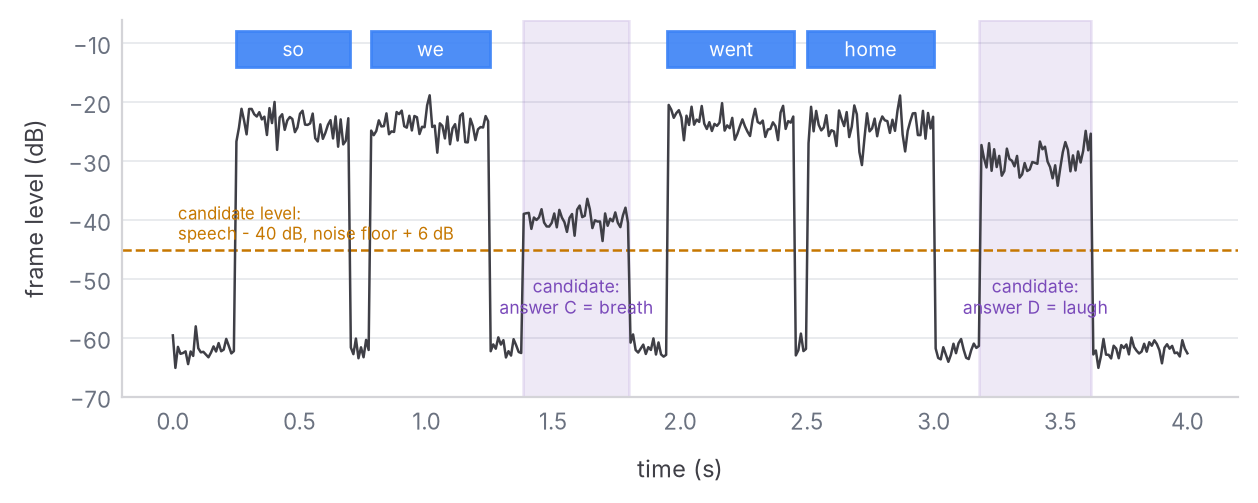
\includegraphics[width=\linewidth]{img/fig_gapmethod.png}
\caption{Where by acoustics, what by an audio language model. Illustration on a synthetic signal.}
\label{fig:gapmethod}
\end{figure}

Figures~\ref{fig:nvprecision}, \ref{fig:nvrecall} and \ref{fig:nvplace} compare the approaches on the test
split; the last of them, our own classifier, is described below.

\begin{figure}[H]
\centering
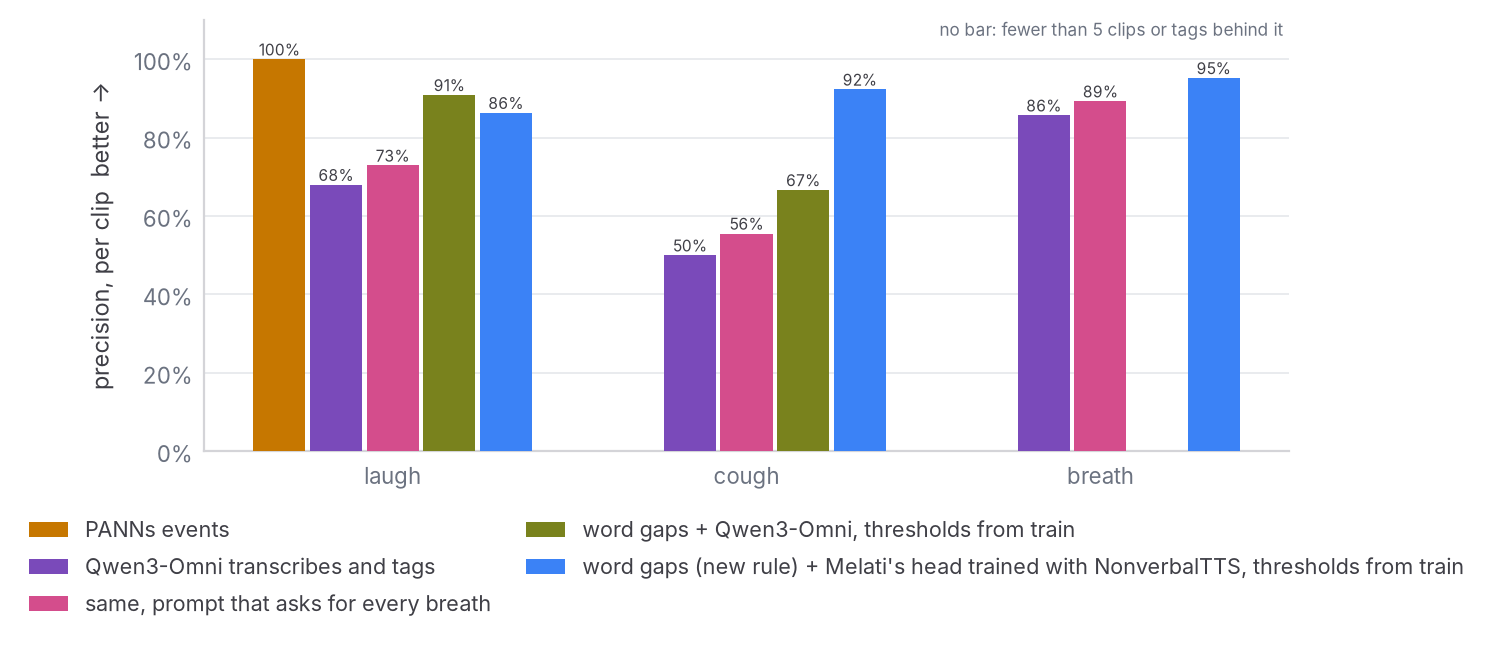
\includegraphics[width=\linewidth]{img/fig_nv_precision.png}
\caption{Precision: of the clips a method says contain the sound, the share that do.}
\label{fig:nvprecision}
\end{figure}

\begin{figure}[H]
\centering
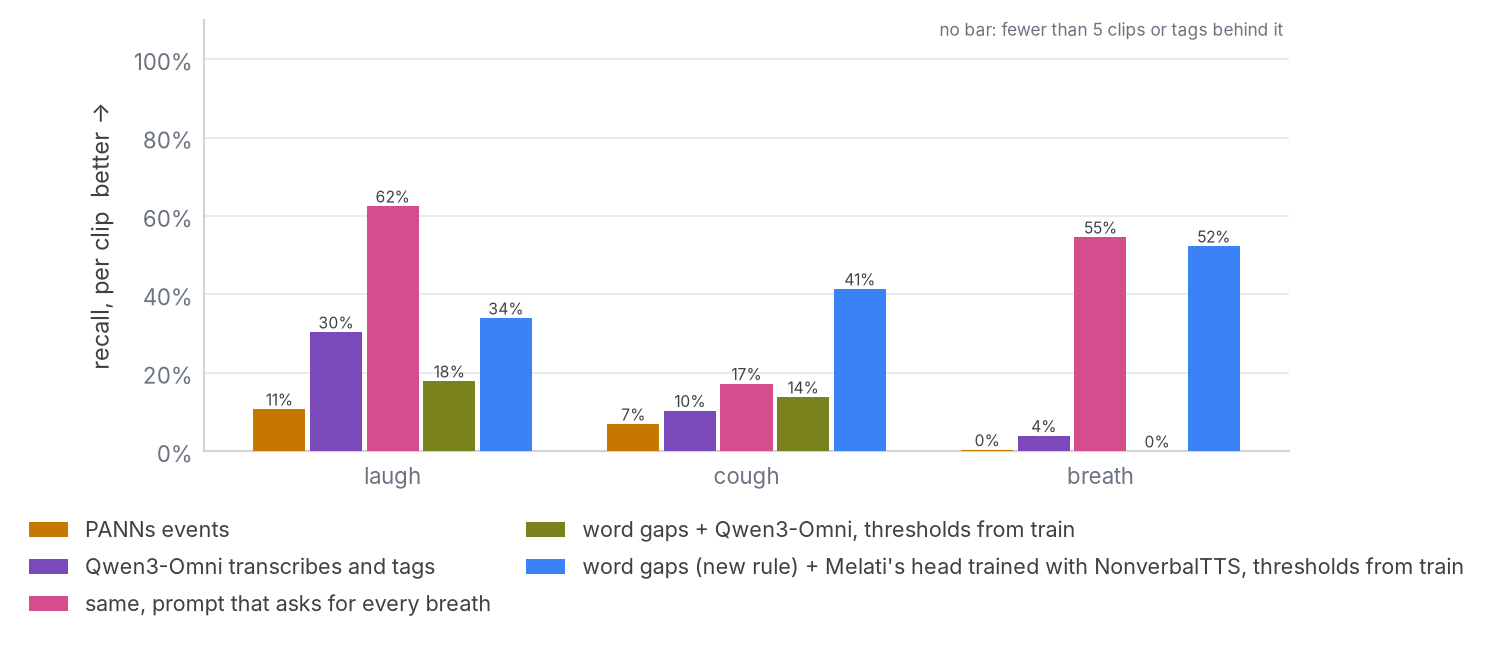
\includegraphics[width=\linewidth]{img/fig_nv_recall.png}
\caption{Recall: of the clips that contain the sound, the share a method finds.}
\label{fig:nvrecall}
\end{figure}

\begin{figure}[H]
\centering
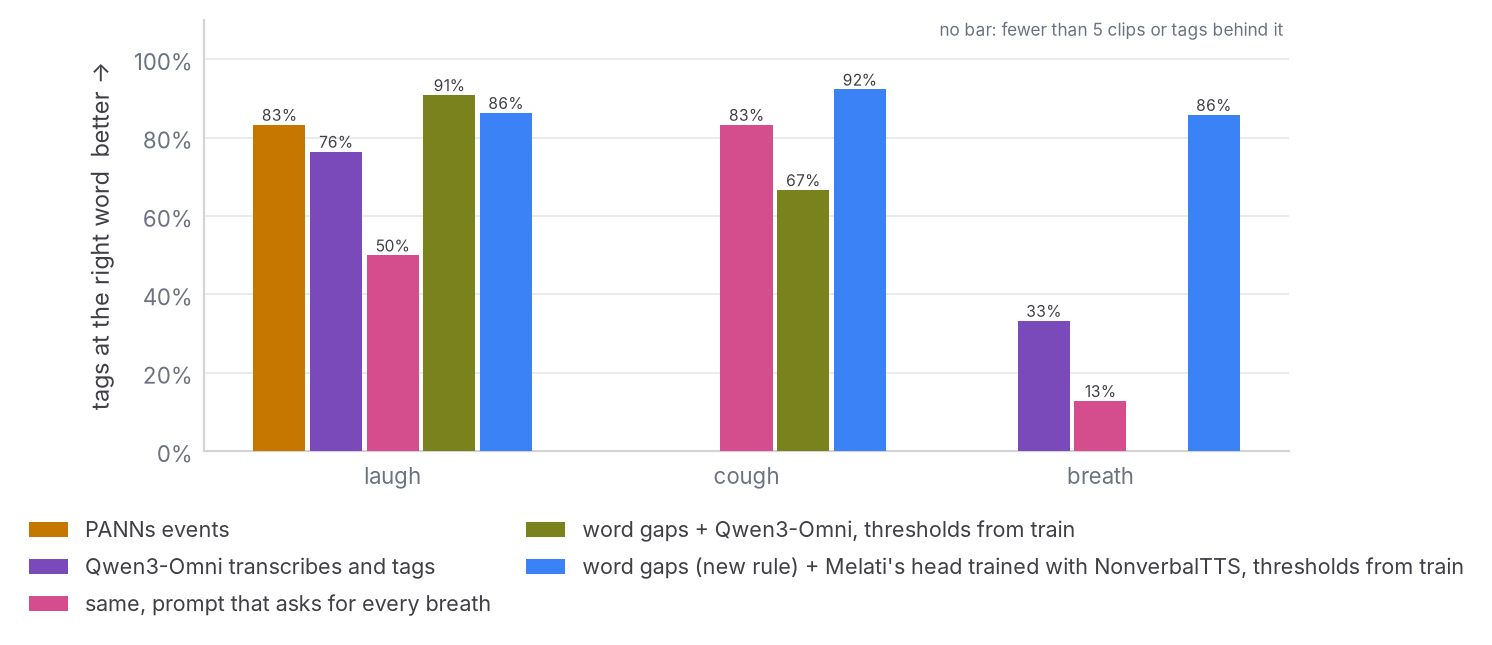
\includegraphics[width=\linewidth]{img/fig_nv_place.png}
\caption{Tags at the right word: the share of a method's tags within one word of a reference tag of their
class.}
\label{fig:nvplace}
\end{figure}

Qwen3-Omni tags laughs at \val{nv/gap/laugh/tagp} precision (threshold \val{nv/thr/laugh}) and coughs at
\val{nv/gap/cough/tagp} (\val{nv/thr/cough}). Recall is the cost: \val{nv/gap/laugh/tagr} of laughs. A laugh over
speech is not in a gap, but most are: \val{nv/gap/laugh/candr} of the reference laughs have a candidate at their
boundary, so it is the labeller that passes most of them up. Its breaths never reach \val{nv/target} on the
training clips (Figure~\ref{fig:nvcurves}), so it tags none.

\begin{figure}[H]
\centering
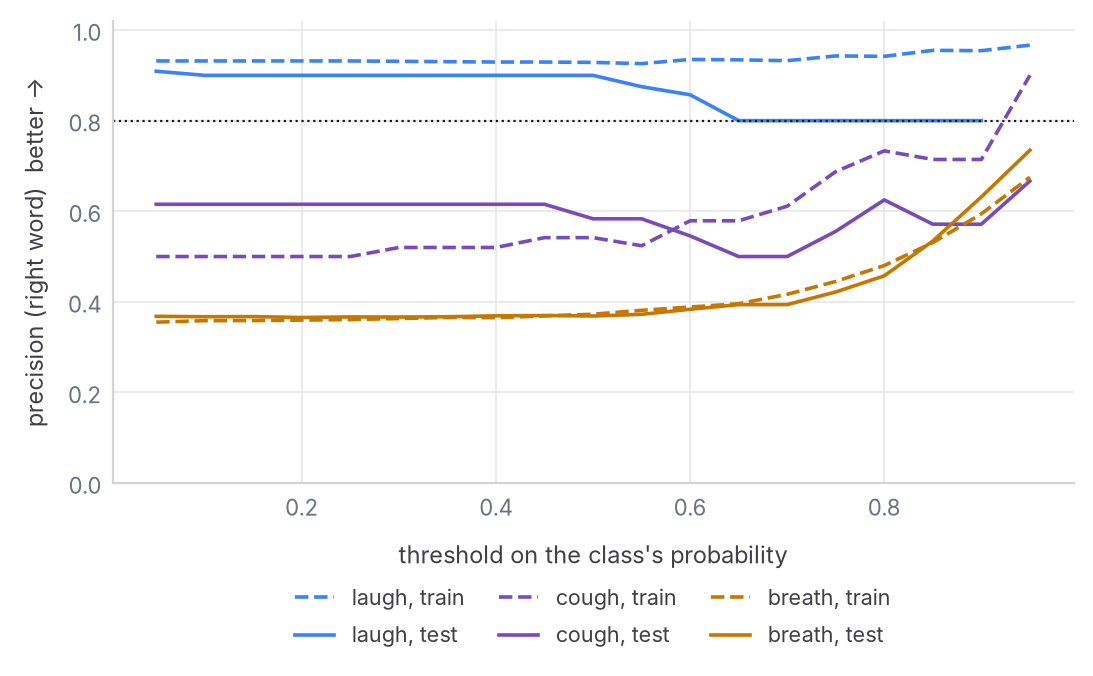
\includegraphics[width=0.86\linewidth]{img/fig_nv_curves.png}
\caption{Tag precision against threshold, training clips (dashed) and test clips (solid). The dotted line is the
bar for tagging.}
\label{fig:nvcurves}
\end{figure}

\paragraph{Our own classifier.} So we replaced the labeller with the emotion heads' design (a learned mix of a
frozen encoder's layers, mean-pooled over the clip, one hidden layer) and an output for each of speech, filler,
breath, laugh, cough, sigh, sniff, throat clearing, sneeze, noise and \emph{other}, a gap sound no annotator tagged.
Trained on hand-cut events alone, the training episodes of PodcastFillers \citep{zhu2022podcastfillers}
(English podcasts with every filler, laugh and breath timed by hand) and VocalSound's \citep{gong2022vocalsound}
recordings, the head on Whisper-large-v3 tells held-out events apart (macro F1 \val{nvhe/whisper/f1}) and real
candidates badly: averaged with heads on WavLM-large and AST \citep{gong2021ast}, its laughs on NonverbalTTS are
\val{nvhe/gap/mix/laugh/tagp} precise and its breaths almost never clear their threshold. A candidate is whatever
an energy rule cuts out of a word gap, mostly word tails and clicks that no one cut by hand. So the training set
gained the candidates themselves: \val{nvh/n/pfc} from PodcastFillers' training episodes, found by the pipeline's
own rule over the word times its transcripts carry and labelled by the hand-timed event each overlaps, and
\val{nvh/n/nvc} from NonverbalTTS training clips outside the 800 that choose the thresholds, labelled by the tag at
their boundary or as \emph{other}; \val{nvh/n/train} clips in all (Figure~\ref{fig:nvheads}).

\begin{figure}[H]
\centering
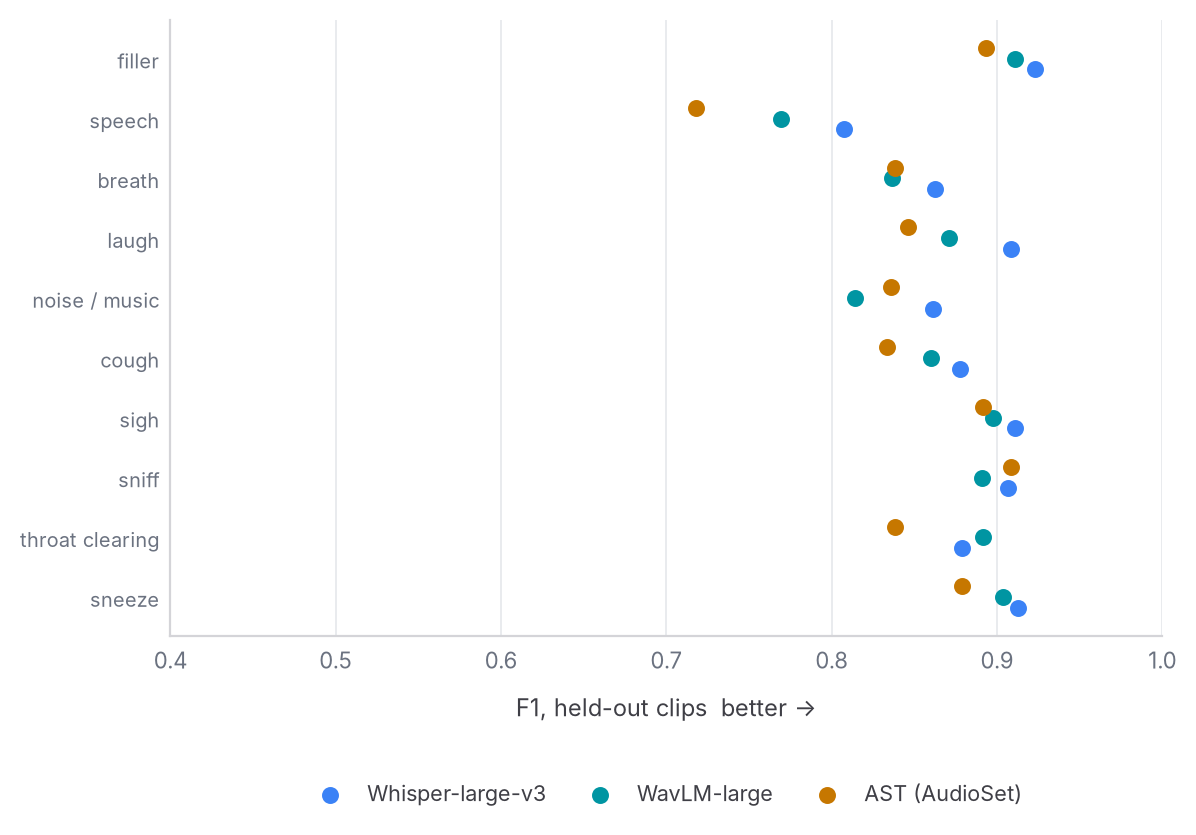
\includegraphics[width=0.86\linewidth]{img/fig_nv_heads.png}
\caption{Each head on events nothing trained on: PodcastFillers' test episodes (shows no model here saw) and
VocalSound's test speakers. F1 at the most probable class.}
\label{fig:nvheads}
\end{figure}

On the same NonverbalTTS test candidates, with thresholds chosen the same way, the head on Whisper-large-v3 tags
\val{nvh/gap/whisper/laugh/tagr} of the laughs at \val{nvh/gap/whisper/laugh/tagp} precision (Qwen3-Omni
\val{nv/gap/laugh/tagr} at \val{nv/gap/laugh/tagp}), \val{nvh/gap/whisper/breath/tagr} of the breaths at
\val{nvh/gap/whisper/breath/tagp}, and \val{nvh/gap/whisper/cough/tagr} of the coughs at
\val{nvh/gap/whisper/cough/tagp} (Figures~\ref{fig:nvprecision} to~\ref{fig:nvplace}). The three heads averaged
do worse (laughs \val{nvh/gap/mix/laugh/tagp} precise), so the pipeline runs the Whisper head alone: one encoder on
the tag server where Qwen3-Omni took a GPU of its own.

\paragraph{A finder for quiet breaths.} The rest of the breaths were lost before any labeller saw them: only
\val{gap/old/found} of the test breaths had a candidate. Hardly any of the others lack a gap
(\val{gap/old/nogap/n} of \val{nv/ref/breath}); they sit in real gaps, too brief above the level threshold
(\val{gap/old/brief/n}) or under it (\val{gap/old/quiet/n}), by a median \val{gap/old/quiet_db} dB
(Figure~\ref{fig:nvmiss}). The threshold that bound was the noise floor's, never the speech level's: these are
interview recordings, and a breath is barely above the room. With the floor margin at 2 dB instead of 6,
\val{gap/new/candr} of the test breaths have a candidate, at \val{gap/new/per_clip} candidates per clip instead of
\val{gap/old/per_clip}. The head was retrained on what the looser rule finds, and the rule chosen on the
calibration clips alone; it tags \val{nv3/breath/tagr} of the test breaths at \val{nv3/breath/tagp} precision,
\val{nv3/cough/tagr} of the coughs at \val{nv3/cough/tagp}, and \val{nv3/laugh/tagr} of the laughs at
\val{nv3/laugh/tagp} (Figure~\ref{fig:nvrules}).

\begin{figure}[H]
\centering
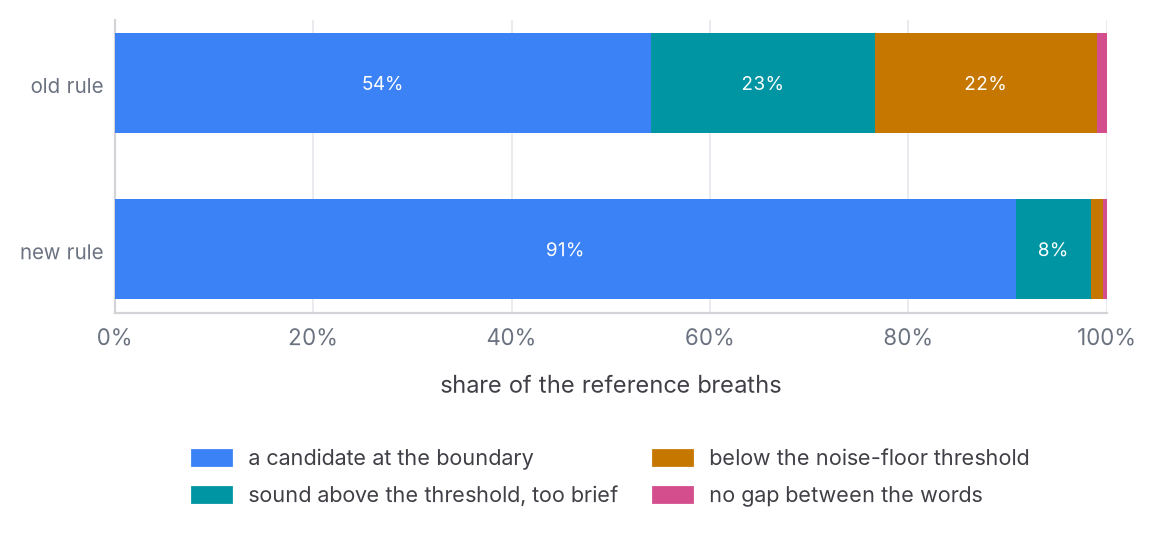
\includegraphics[width=0.9\linewidth]{img/fig_nv_miss.png}
\caption{The NonverbalTTS test breaths, by what the gap finder made of them: a candidate within one word, sound in
the gap above the threshold for under 80 ms, sound under it, or no gap between the words at all.}
\label{fig:nvmiss}
\end{figure}

\begin{figure}[H]
\centering
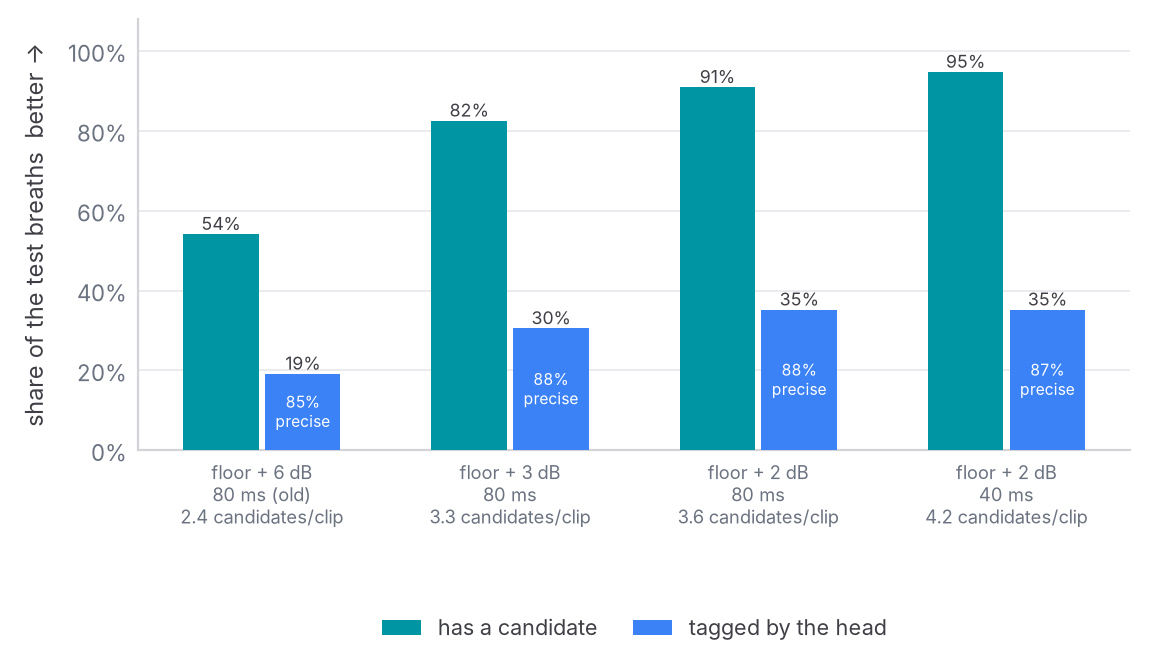
\includegraphics[width=0.92\linewidth]{img/fig_nv_rules.png}
\caption{Each candidate rule on the NonverbalTTS test breaths: the share with a candidate, and the share tagged by
the head retrained on the loosest rule's candidates, at thresholds chosen on the calibration clips.}
\label{fig:nvrules}
\end{figure}

\paragraph{The released model.} PodcastFillers' annotations are licensed for non-commercial research only, and
the sources beside them must allow that in one set of weights: VocalSound is CC BY-SA, and so are 79 of
PodcastFillers' own 199 episodes, with 20 more CC BY-ND. NonverbalTTS is the third: its metadata says Apache-2.0,
but its README licenses the annotations CC BY-NC-SA, so the head above, which trained on its candidates, cannot be
released. Without them, a head trained on PodcastFillers' CC BY episodes and COUGHVID's coughs
\citep{orlandic2021coughvid} must raise its thresholds to \val{nonv/thr/laugh} to reach \val{nv/target} precision on
NonverbalTTS's training clips, and then finds \val{nonv/nv/laugh/tagr} of the test laughs: those interviews are a
domain of their own, which only their own candidates taught. So the released model is calibrated where Melati
works, on podcasts: its breath threshold is the lowest giving \val{nv/target} precision where PodcastFillers'
validation episodes have a label (\val{rel/thr/breath}). Its gap head trains on
PodcastFillers' CC BY episodes, AMI's meetings \citep{carletta2005ami} (CC BY 4.0: \val{rel/n/amic} gap candidates
its transcribers marked and \val{rel/n/amiu} they did not, as \emph{other}), and the coughs of COUGHVID and Coswara
\citep{bhattacharya2023coswara} (CC BY 4.0). It tags breaths only. Its own laugh tags in podcasts come at twice the
first head's rate for the same recall, and AudioSet's classifier hears the extra ones as gasps:
\val{audit/laugh/gap/unl/gasp} of its unlabelled laugh tags have Gasp as their top class, and they score
\val{audit/laugh/gap/unl} on Laughter against \val{audit/laugh/gap/hand} for hand-labelled laughs. On NonverbalTTS, now
out of domain, it tags \val{rel/nv/breath/tagr} of the breaths at \val{rel/nv/breath/tagp} precision (the first
head, trained there: \val{prev/nv/breath/tagr} at \val{prev/nv/breath/tagp}). Laughs and coughs come from a
second head, below. Both are released as one checkpoint at
\url{https://huggingface.co/Scicom-intl/Melati-NonVerbal-Whisper-Large-V3} for non-commercial research.

\paragraph{Laughs and coughs over speech.} A gap finder only looks between words. In AMI's test meetings,
\val{ami/laugh/nocand_speech} of the \val{ami/laugh/n} marked laughs and \val{ami/cough/nocand_speech} of the
\val{ami/cough/n} coughs lie over someone's words with no candidate at all, and the first head found
\val{ami/prev/laugh/r} of the laughs and none of the coughs. A frame-level head reads the whole segment instead:
eight layers of the same frozen encoder averaged to ten frames a second, a learned mix of them, and four residual
dilated convolutions over time (about 6 s of context), giving every 0.1 s an independent probability of laughter,
a cough, another vocal sound and speech. AMI marks every word and every laugh of its conversations, so there a
frame with no mark is a negative; PodcastFillers' CC BY training episodes add podcasts, their classes known only
inside the regions its annotators labelled. A run of frames over the threshold is an event: laughs at
\val{frm/thr/laugh}, chosen on PodcastFillers' validation episodes, and coughs at \val{frm/thr/cough}, chosen on
AMI's dev meetings, since PodcastFillers labels none. It finds \val{frm/pf/laugh/r} of the \val{frm/pf/laugh/n}
hand-timed laughs in PodcastFillers' test episodes, \val{frm/pf/laugh/p} precise where labelled; \val{frm/ami/laugh/r}
of AMI's test laughs at \val{frm/ami/laugh/p} (\val{frm/ami/laugh/rs} of those over speech) and
\val{frm/ami/cough/r} of its coughs at \val{frm/ami/cough/p}; and, out of domain, \val{frm/nv/laugh/r} of
NonverbalTTS's laughs at \val{frm/nv/laugh/p} (Figure~\ref{fig:nvframes}). NonverbalTTS's coughs it does not find:
it learnt coughs from meetings, and adding COUGHVID's and Coswara's phone recordings to its training lowered AMI's
to \val{frm4/ami/cough/r} without reaching NonverbalTTS's. The pipeline takes laughs and coughs from this head,
adding an event wherever the gap head tagged none of its kind within 0.3 s.


\begin{figure}[H]
\centering
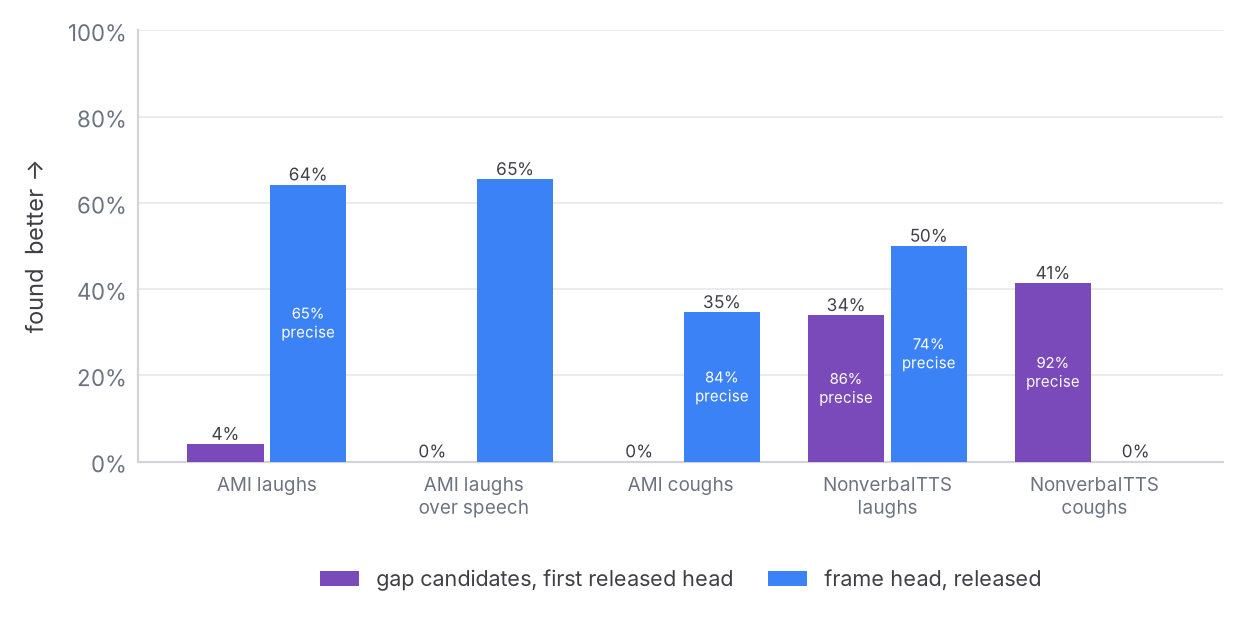
\includegraphics[width=\linewidth]{img/fig_nv_frames.png}
\caption{Laughs and coughs found by the first released head on gap candidates and by the frame-level head, each at
the thresholds it ships with; precision written in the bar. AMI's test meetings: a tag is right where the
transcribers marked its class within 0.1 s. NonverbalTTS's test split: within one word of a reference tag.}
\label{fig:nvframes}
\end{figure}


On PodcastFillers' test episodes, through the whole pipeline (Figure~\ref{fig:nvpf}), the released model finds
\val{fill/nvw/inside/laughter/r} of the laughs inside what Melati keeps (the first head
\val{fill/nvp/inside/laughter/r}, Qwen3-Omni \val{fill/rel/inside/laughter/r}) and \val{fill/nvw/inside/breath/r}
of the breaths (the first head \val{fill/nvp/inside/breath/r}). As scored,
\val{fill/nvw/inside/laughter/p} of its laugh tags and \val{fill/nvw/inside/breath/p} of its breath tags are right,
but PodcastFillers labels only the regions its own detector proposed, and \val{fill/nvw/unl/breath} of the
\val{fill/nvw/inside/breath/pred} breath tags fall where it has no label at all. Where it has one,
\val{fill/nvw/lab/laughter/p} of the laugh tags (Qwen3-Omni's \val{fill/rel/lab/laughter/p}) and
\val{fill/nvw/lab/breath/p} of the breath tags are right. The unlabelled breath tags sound to AudioSet's own
classifier like hand-labelled breaths: \val{audit/breath/unl} have a gasp, a sigh or a snort as its top class, against
\val{audit/breath/hand} of hand-labelled breaths and \val{audit/breath/words} of hand-labelled words. The looser
gap finder is what adds those: the old rule, with a head trained on VocalSound, made \val{fill/nvw2/inside/breath/pred}
breath tags, \val{fill/nvw2/unl/breath} of them unlabelled, and found about as many of the breaths PodcastFillers did
label as the first released head under the new rule (\val{fill/nvw2/inside/breath/r} against
\val{fill/nvp/inside/breath/r}): the breaths its detector proposed are the louder ones, which the old rule already
reached. The released model's gap head, calibrated on podcasts, finds more of them at the same precision. On the 200 Malaysian podcasts of Section~\ref{sec:cmp} the export
carries \val{pev/head/breathes/h} breath tags an hour (the first head \val{pev/prev/breathes/h}, \val{pev/old/breathes/h}
with the old rule; Qwen3-Omni tagged none) and \val{pev/head/laughs/h} laugh tags (the first head
\val{pev/prev/laughs/h}, Qwen3-Omni \val{pev/qwen/laughs/h}), and no cough tags: the frame head's cough threshold,
chosen on AMI's meetings, is never reached there (the first head tagged \val{pev/prev/coughs/h} an hour). Coughs
remain the class no licence-clean source measures in podcasts.

\begin{figure}[H]
\centering
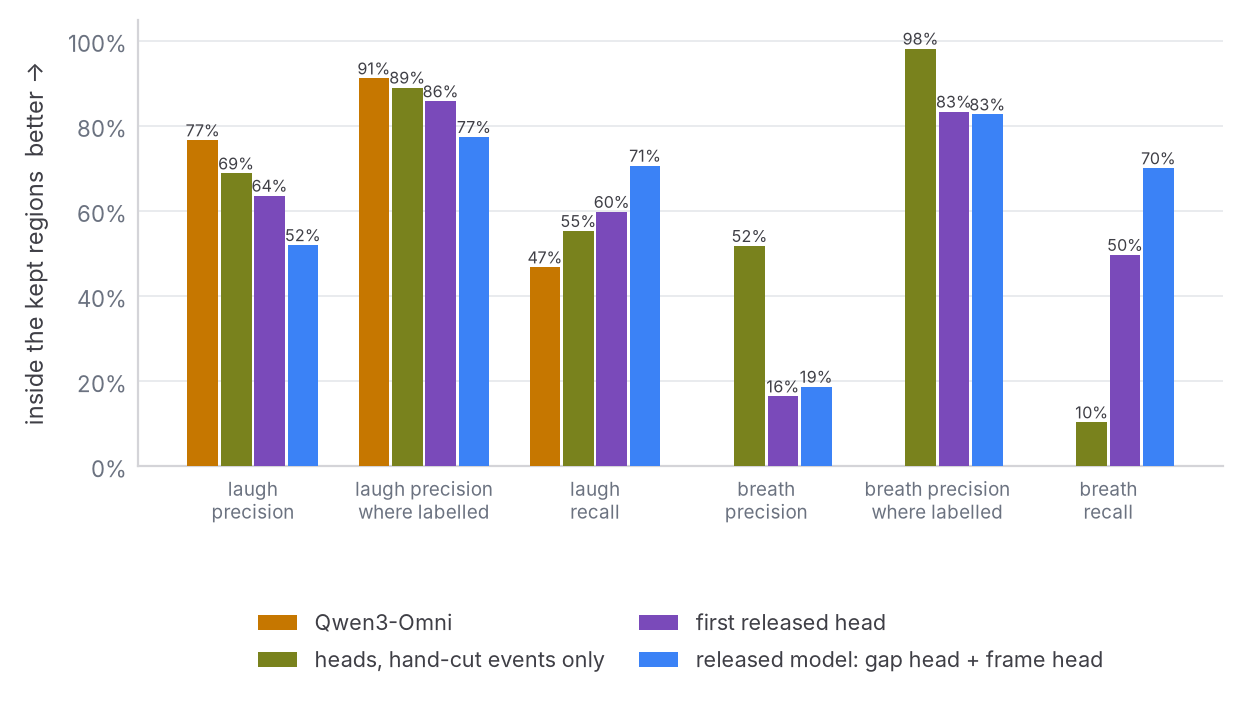
\includegraphics[width=0.9\linewidth]{img/fig_nv_pf.png}
\caption{PodcastFillers test episodes through the pipeline, inside the regions Melati exports: the same gap
candidates labelled by Qwen3-Omni, by heads trained on hand-cut events only and by the first released head, each at
thresholds chosen on NonverbalTTS training clips; and the released model, breaths from its gap head and laughs from
its frame head, at thresholds chosen on PodcastFillers' validation episodes. Precision as scored counts a tag where
PodcastFillers has no label as wrong; where labelled counts only the tags that overlap one of its labels.}
\label{fig:nvpf}
\end{figure}

Melati v1 tags laughs at \val{frm/ds/thr}, the threshold AMI's dev meetings choose: on PodcastFillers' test episodes
through the pipeline it finds \val{frm/sweep/ds/r} of the laughs, \val{frm/sweep/ds/p} precise where labelled, where
the \val{frm/thr/laugh} the head ships with finds \val{frm/sweep/ship/r} at \val{frm/sweep/ship/p}. The first
released head (\val{frm/sweep/prev/r} at \val{frm/sweep/prev/p}) and Qwen3-Omni (\val{frm/sweep/omni/r} at
\val{frm/sweep/omni/p}) lie on the same curve (Figure~\ref{fig:laughsweep}): their higher precision is a stricter
threshold, which this head reaches too. A wrong laugh teaches a voice to laugh at the wrong moment, where a missing
one only teaches less, so the dataset takes the stricter threshold, and adds the laughs AudioSet's taggers hear (below).

\begin{figure}[H]
\centering
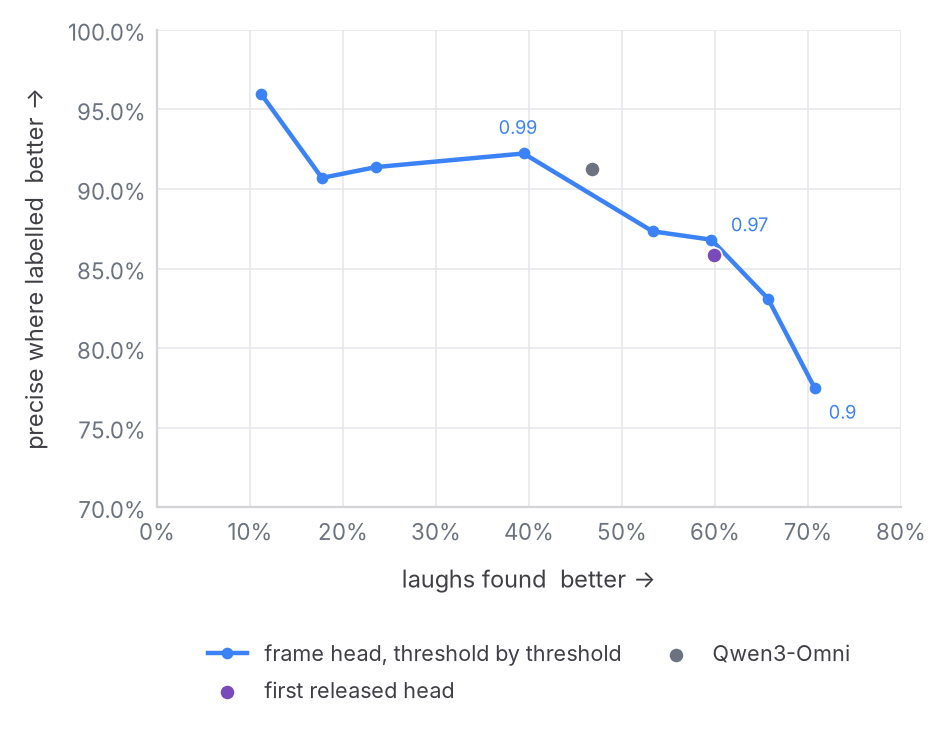
\includegraphics[width=0.62\linewidth]{img/fig_laugh_sweep.png}
\caption{Laughs in PodcastFillers' test episodes through the pipeline, at every threshold of the frame head; the
first released head and Qwen3-Omni at the thresholds they ship with. Precision counts only tags where PodcastFillers
has a label.}
\label{fig:laughsweep}
\end{figure}

\paragraph{AudioSet's taggers.} Three of the frame-level models \citet{schmid2025effective} fine-tuned on AudioSet's
time-stamped labels \citep{gemmeke2017audioset}, BEATs, ATST-F and M2D (447 classes every 40 ms), averaged frame by
frame, hear sounds no head here was trained for. On NonverbalTTS's \val{as/nvtts/clips} clips (\val{as/nvtts/h}
hours, none of which they trained on), with each threshold chosen on one half for 80\% precision and measured on the
other, sniffs at \val{as/sniff/t} are \val{as/sniff/p} precise and \val{as/sniff/r} found, throat clearing at
\val{as/throat_clear/t} is \val{as/throat_clear/p} precise and \val{as/throat_clear/r} found, and coughs at
\val{as/cough/t} are \val{as/cough/p} precise and \val{as/cough/r} found, where the frame head finds none of
NonverbalTTS's coughs
(Figure~\ref{fig:audioset}). On Expresso they mark \val{as/whisper/found} of the whispered utterances and
\val{as/whisper/others} of the \val{as/whisper/n_others} in its other styles, so whispering is a delivery tag over
the words it covers. Their laughs at \val{as/laugh/t}, added to the frame head's at \val{frm/ds/thr}, find
\val{as/union/r} of PodcastFillers' test laughs through the pipeline, \val{as/union/p} precise where labelled: as
many as the head alone at \val{frm/thr/laugh} (\val{frm/sweep/ship/r}), at its stricter precision. Sneezes and groans
hold 80\% on neither half, gasps land on labelled breaths and laughs, breathing fires on every sound, and sighs,
crying, humming, singing and shouting are almost never heard in the podcasts, so none of them is tagged.

\begin{figure}[H]
\centering
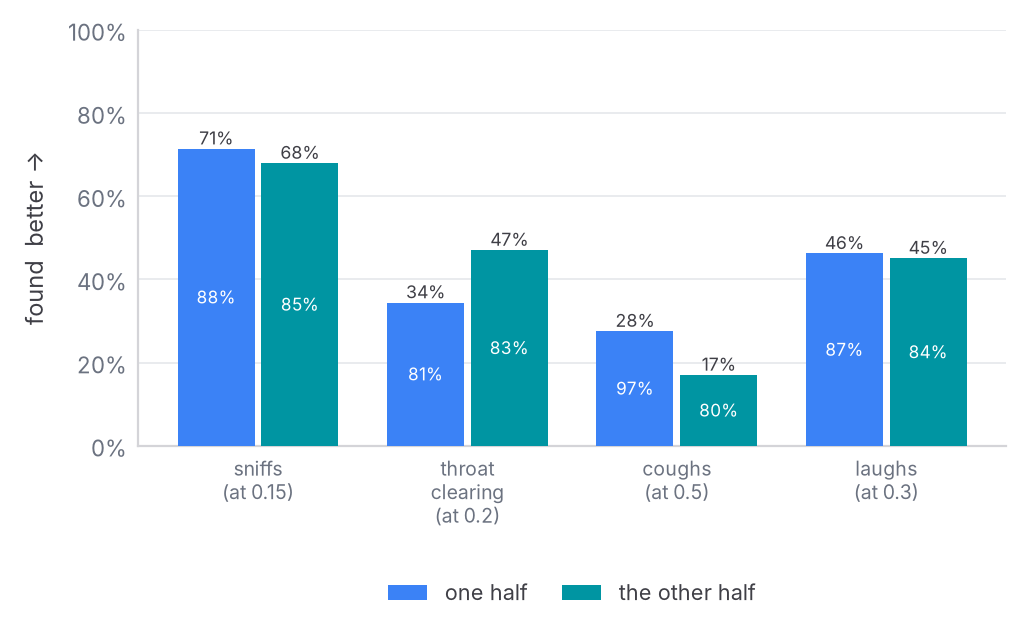
\includegraphics[width=0.72\linewidth]{img/fig_audioset.png}
\caption{AudioSet's taggers on NonverbalTTS at the thresholds Melati v1 tags at: found in each half of the clips
(over the bar), each threshold chosen on the other half for 80\% precision; precision written in the bar. A tag is
right within one word of a reference tag of its class.}
\label{fig:audioset}
\end{figure}

\subsection{Fillers}

A filler reaches the transcript two ways: Whisper writes it ("um", "erm"), or stage H transcribes a voiced gap
on its own and the result is a filler. Stage H depends on the fine-tune: a model that writes text over a breath
would turn every gap into a word.

We scored them on PodcastFillers \citep{zhu2022podcastfillers}, English podcasts with every "uh" and "um",
laugh and breath timed by hand. Melati ran on its \val{fill/episodes} test episodes (shows no model here trained
on) twice, once with base whisper-large-v3 and once with the released model (Section~\ref{sec:asr}), everything else the same; a tag
counts when it lands within \val{fill/tol_ms} ms of a label of its class (Figure~\ref{fig:fillers}).

\begin{figure}[H]
\centering
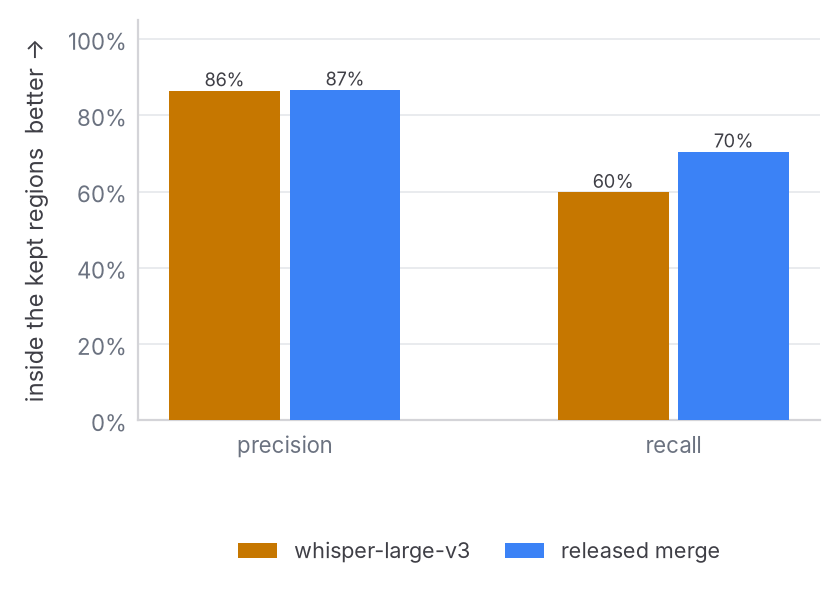
\includegraphics[width=0.9\linewidth]{img/fig_fillers.png}
\caption{PodcastFillers test episodes, inside the regions Melati exports: the fillers it wrote, against the hand
labels, with base Whisper and with the released model.}
\label{fig:fillers}
\end{figure}

With base, Melati finds \val{fill/base/inside/filler/r} of the fillers inside what it keeps, at
\val{fill/base/inside/filler/p} precision; with the released model, \val{fill/rel/inside/filler/r} at
\val{fill/rel/inside/filler/p}: it writes the fillers base leaves out, at the same precision. Laughs and breaths
are the non-verbal head's (Figure~\ref{fig:nvpf}). Over whole episodes filler recall is lower
(\val{fill/rel/all/filler/r} of \val{fill/all/filler/ref} fillers), because export leaves out what it cannot keep
cleanly: overlapped speech, music, the edges of a cut.

\subsection{An AudioSet tagger}
\label{sec:astagger}

The dataset's AudioSet tags come from PretrainedSED's frame-level models (above). For tagging whole clips we also
trained a tagger of our own, and released it. First we scored six released clip taggers on the same clips: the
\val{astag/clips} clips of AudioSet's evaluation set that agkphysics/AudioSet holds today. YouTube removes clips over
time, so every paper's copy differs and published numbers do not compare across papers. Each model ran in fp32 with
its own preprocessing. CED-base \citep{dinkel2024ced} leads at \val{astag/m/ced-base} mAP, ahead of EAT-large
\citep{chen2024eat} at \val{astag/m/eat-large} and SSLAM \citep{alex2025sslam} at \val{astag/m/sslam}, and the average of
those three reaches \val{astag/avg} (Figure~\ref{fig:asmap}). BEATs \citep{chen2023beats} scores \val{astag/m/beats}.
bf16 lowers each tagger's score by at most \val{astag/bf16gap} of a point, so training evaluates in bf16 and every
number reported is fp32.

\begin{figure}[H]
\centering
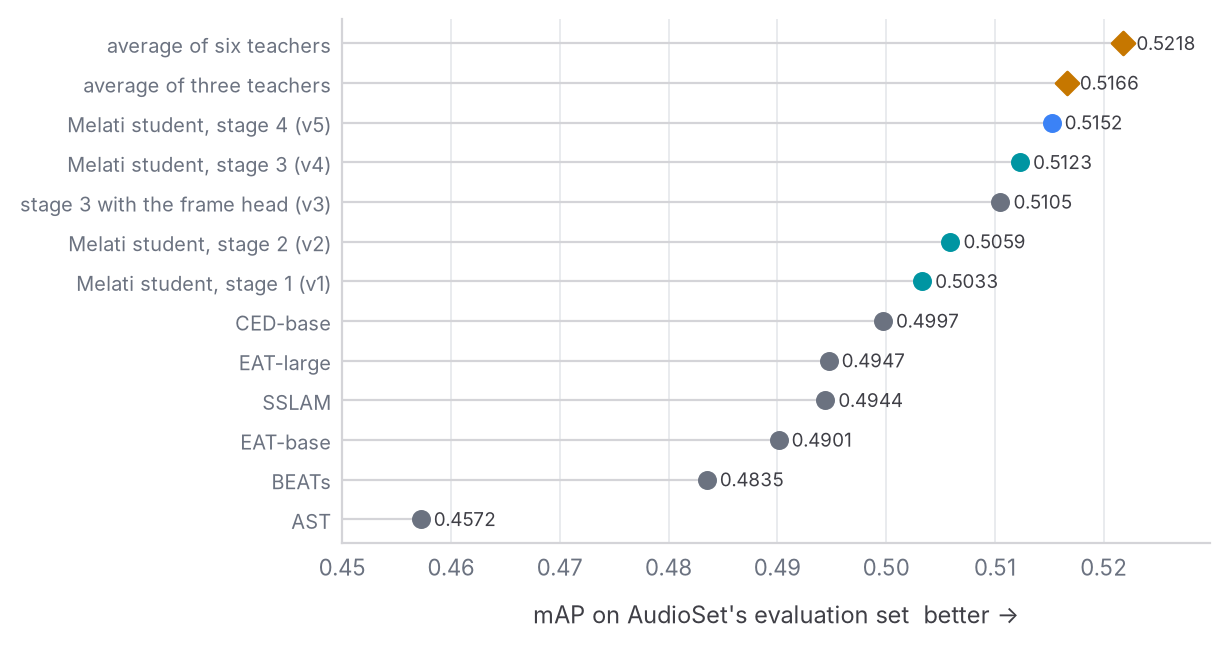
\includegraphics[width=0.72\linewidth]{img/fig_as_map.png}
\caption{AudioSet taggers on the same \val{astag/clips} evaluation clips, in fp32: six released models, the two averages
the student learned from (three teachers for stages 1 to 3, six for stage 4), the student after each stage of
training, and stage 3 trained with the frame head beside it. In brackets, the version each student was released as.}
\label{fig:asmap}
\end{figure}

The student is EAT-large, trained to its teachers' average probability for each class with binary cross-entropy:
the three taggers above for three stages, and six for the fourth (below). AudioSet's own clip labels are not used,
and no clip of the evaluation set is trained on. Four stages took it from EAT-large's own \val{astag/m/eat-large} to
\val{astag/s4} (Figure~\ref{fig:astrain}):
\begin{enumerate}
\item \val{astag/s1/epochs} epochs on AudioSet's strongly labelled training clips (\val{astag/pool/clean/strong}, every
  event timed by hand) and its balanced set (\val{astag/pool/clean/bal}): \val{astag/s1}, already above every released
  model.
\item \val{astag/s2/epochs} epochs with \val{astag/pool/big/unbal} clips of the unbalanced set added
  (\val{astag/pool/big/clips} clips, \val{astag/pool/big/h} hours): \val{astag/s2}.
\item \val{astag/s3/epochs} epochs on the first set again, without mixup: \val{astag/s3}.
\item \val{astag/s4/epochs} epochs on the second set again, without mixup, toward six teachers: \val{astag/s4}.
\end{enumerate}

\begin{figure}[H]
\centering
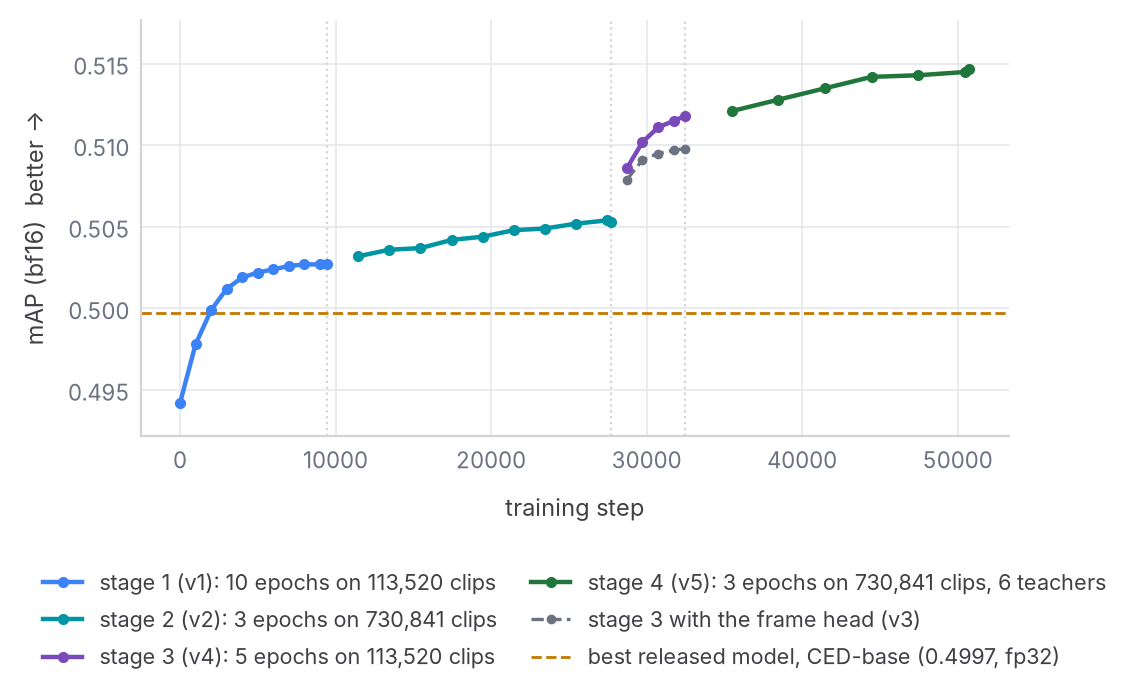
\includegraphics[width=0.72\linewidth]{img/fig_as_train.png}
\caption{The student's mAP at each evaluation (bf16, the moving average of its weights), stage after stage. Grey
dashes: stage 3 trained with the frame head beside it. Orange dashes: the best released model, in fp32. In brackets, the
version each stage was released as.}
\label{fig:astrain}
\end{figure}

Stage 3 was first trained with a second head beside the first. That head reads the encoder's tokens every 160 ms
and learns where each sound is from the hand-timed events. With it, the clip head reached \val{astag/fh/clip}.
Trained again with only that loss switched off, stage 3 reaches \val{astag/s3}. So the timed events did not lift
the clip head. The lift over stage 2 comes from the rest of the stage: another learning-rate cycle on the first set,
without mixup. The frame head also places sounds less well than PretrainedSED: on the \val{astag/frm/clips}
strongly labelled test clips its frame mAP is \val{astag/frm/ours}, against \val{astag/frm/psed} for PretrainedSED's
average, over the \val{astag/frm/classes} classes both have. So stage 3 was released without the frame head.

A tag in a transcript also needs to know where its sound is. Read off 2 s windows, the stage 3 tagger scores
\val{astag/win/v4} frame mAP on those test clips, barely above the \val{astag/win/clip} it scores by giving every
160 ms its probability for the whole clip. The mean of PretrainedSED's taggers and the frame head scores
\val{astag/win/mean}, above either alone. Weighting it by the stage 3 tagger's probability for the clip lowers it
(\val{astag/win/gated} for PretrainedSED). So the dataset's sound tags take which sounds a segment holds from the
stage 3 tagger, and where they are from that mean (Section~\ref{sec:dataset}).

A larger student did not help. Dasheng-1.2B \citep{dinkel2024dasheng} is a self-supervised encoder nearly four
times EAT-large's size, with no AudioSet training of its own. Given a new head and the same \val{astag/pool/big/clips} clips, it
reached \val{astag/dash} after \val{astag/dash/epoch} of its \val{astag/dash/epochs} epochs (step
\val{astag/dash/step}), and we stopped it there: its last \val{astag/dash/every} steps had added
\val{astag/dash/last}. EAT-large starts from a model already trained on AudioSet (\val{astag/m/eat-large} on its
own).

Better teachers did help. A student learns its teachers' average, and stage 3 ended \val{astag/gap3} of a point under
the three's, so we looked for teachers that raise it. Stage 3 and its frame-head twin, added to the three, lift the
average to \val{astag/t/v3v4}. BEATs, the weakest of them alone, lifts the three to \val{astag/t/beats}; it was
pre-trained differently from the rest. PretrainedSED's frame taggers, read at clip level (each class's highest frame),
score \val{astag/t/psed/lo} to \val{astag/t/psed/hi} and lower every one of the \val{astag/t/psed/n} averages they
join (the three's to \val{astag/t/psed/three} at best). All six average \val{astag/avg6}. Stage 4 trains stage 3
toward that average, reaching \val{astag/s4}: \val{astag/lift4} of a point above stage 3 and still \val{astag/gap} of a
point under its teachers. That is v5, the current release, under MIT as EAT is:
\url{https://huggingface.co/Scicom-intl/Melati-AudioSet-EAT-Large}. The earlier stages were released there before it:
stages 1 and 2 as v1 and v2, stage 3's frame-head twin as v3 and stage 3 as v4.

The six teachers' average is released as well, each model run with its own preprocessing:
\url{https://huggingface.co/Scicom-intl/Melati-AudioSet-Ensemble}. Loaded back from the Hub it scores \val{astag/ens}
in fp32 and \val{astag/ens/bf16} in bf16, for six forward passes and \val{astag/ens/params}B parameters; the
\val{astag/avg6} above averages probabilities stored in 16 bits. CED-base's feature extractor sets its decibel floor
under the loudest clip it is given, so there each clip's floor is set under its own, as for a clip given alone, and
CED-base alone reads \val{astag/ens/ced1} (\val{astag/m/ced-base} in batches of 64).
Left out one at a time, BEATs costs the ensemble most (\val{astag/ens/add/beats}), then CED-base
(\val{astag/ens/add/ced}). EAT-large costs nothing (\val{astag/ens/add/eat}): without it the other five average
\val{astag/ens/five}. Stage 3 and its twin were both trained from it.

The members are rebuilt there in plain PyTorch, so loading the ensemble fetches only their weights and runs none of
their repositories' code. An inference engine ships with it: every GPU holds all six members in bf16, and the 10 s
windows of concurrent requests are batched together. Through it the evaluation set scores \val{astag/eng/map} mAP, at
\val{astag/eng/multi} clips a second on \val{astag/eng/n} GPUs (\val{astag/eng/rt} times real time). One GPU tags
\val{astag/eng/one} a second, about what the plain bf16 call does in batches of 64 (\val{astag/eng/ens64}): a clip
costs \val{astag/eng/tflop} TFLOP, so the GPU's compute is the limit.

\section{Against Emilia-Pipe on the same recordings}
\label{sec:cmp}

We ran upstream Emilia-Pipe, its code unchanged, on two sets: twelve VoxConverse recordings \citep{chung2020spot}
(\val{vox/hours} hours of debates, news and talk shows), whose reference speaker turns measure purity, and 200
Malaysian podcast recordings. Melati is read twice: everything it exports, and the subset upstream's filter
would keep, because Melati filters by query rather than before export.

\subsection{VoxConverse}

Upstream keeps \val{vox/emilia/kept} of the input; Melati exports \val{vox/melati_all/kept}, and its
Emilia-filtered subset \val{vox/melati_emilia_filter/kept} (Figure~\ref{fig:voxyield}). Of the speech in which
exactly one reference speaker talks, Melati keeps \val{vox/melati_all/single}, upstream \val{vox/emilia/single}.
Part of Melati's share is set by its transcriber, because export drops a segment whose transcript is empty: the
released model leaves \val{drops/vox_rel/share} of the \val{drops/vox_rel/segments} segments empty, the Indic + KL
model alone \val{drops/vox_ft/share}, most of them English speech it stopped on (Section~\ref{sec:asr}).

\begin{figure}[H]
\centering
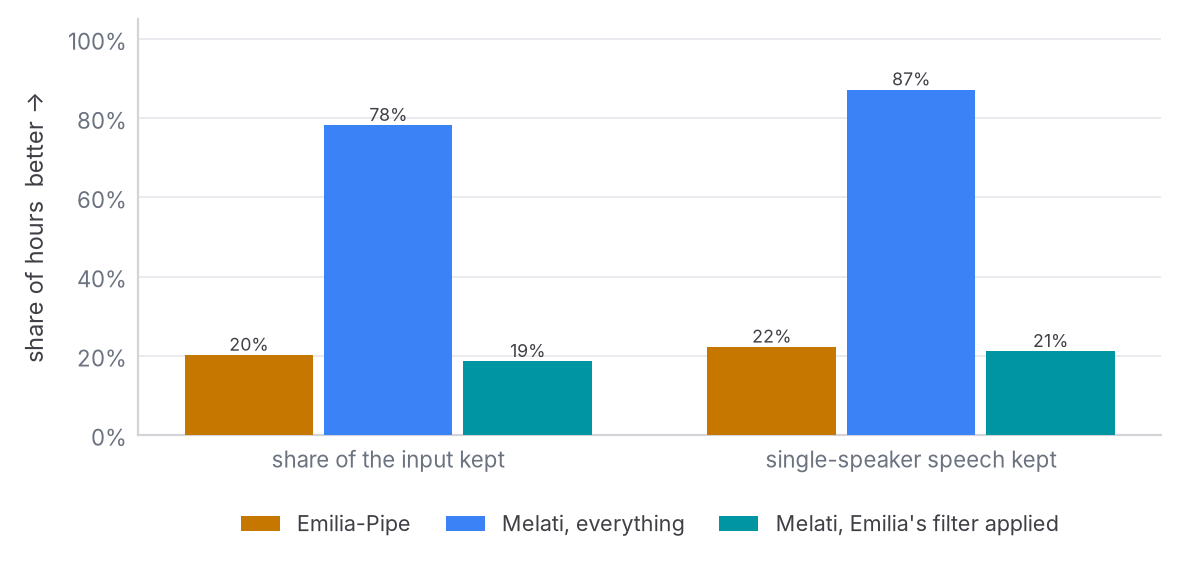
\includegraphics[width=0.92\linewidth]{img/fig_vox_yield.png}
\caption{Hours kept, as a share of the input, and of the reference single-speaker speech.}
\label{fig:voxyield}
\end{figure}

Purity is measured against the reference turns (Figure~\ref{fig:voxpurity}): the share of a segment's reference
speech in which only its main speaker talks, a second speaker present for half a second or more, and overlap of
0.2 s or more.

\begin{figure}[H]
\centering
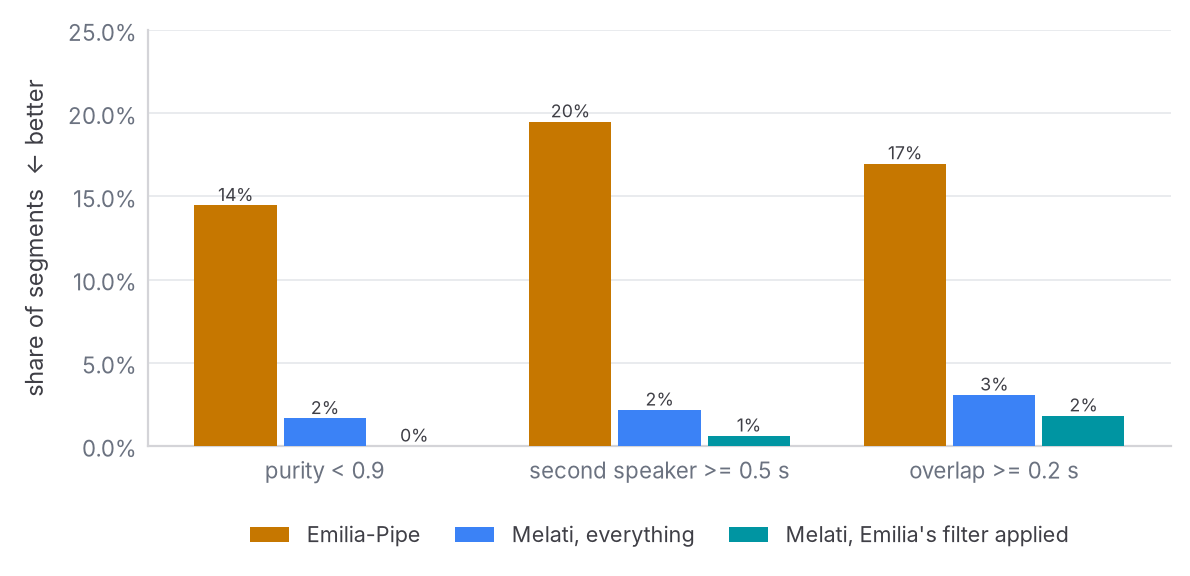
\includegraphics[width=0.92\linewidth]{img/fig_vox_purity.png}
\caption{Segments that carry more than one voice, by three measures.}
\label{fig:voxpurity}
\end{figure}

A segment that starts or ends inside a word pairs audio with text it does not contain. Each pipeline's own
transcript, aligned to its own audio, shows where the first and last words fall (Figure~\ref{fig:voxcut}):
upstream starts mid-word in \val{vox/emilia/firstcut} of its segments, Melati in \val{vox/melati_all/firstcut}.

\begin{figure}[H]
\centering
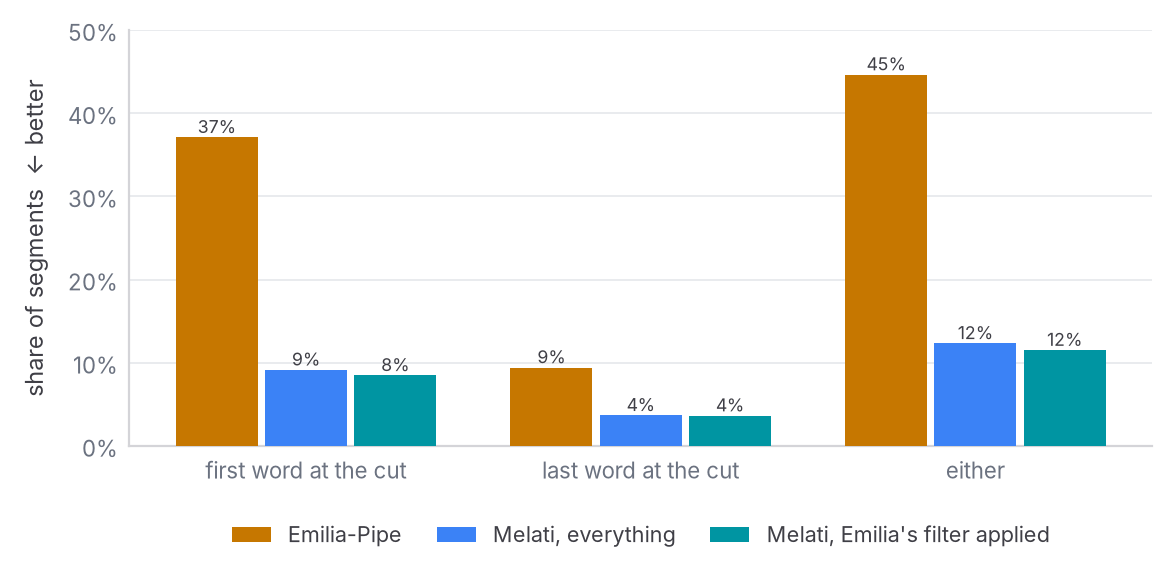
\includegraphics[width=0.92\linewidth]{img/fig_vox_cut.png}
\caption{Segments whose first or last aligned word is within 20 ms of the cut.}
\label{fig:voxcut}
\end{figure}

Melati's segments are shorter, because it cuts in pauses and drops overlap instead of keeping whole turns
(Figure~\ref{fig:voxdur}); \val{vox/melati_all/lt3} of them are under three seconds, a length upstream's filter
removes.

\begin{figure}[H]
\centering
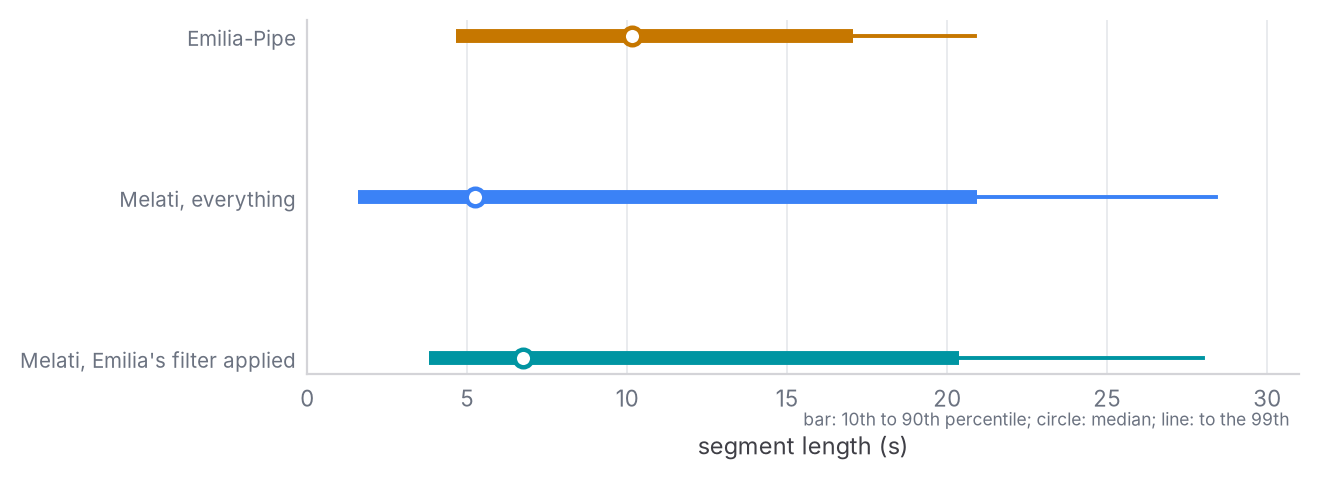
\includegraphics[width=0.86\linewidth]{img/fig_vox_dur.png}
\caption{Segment length per pipeline.}
\label{fig:voxdur}
\end{figure}

\subsection{Malaysian podcasts}

On the 200 podcasts (\val{pil/hours} hours), upstream keeps \val{pil/emilia/kept} of the audio and Melati exports
\val{pil/melati_all/kept}; the part of Melati's export that upstream's own filter would pass is
\val{pil/melati_emilia_filter/kept} (Figure~\ref{fig:pilyield}).

\begin{figure}[H]
\centering
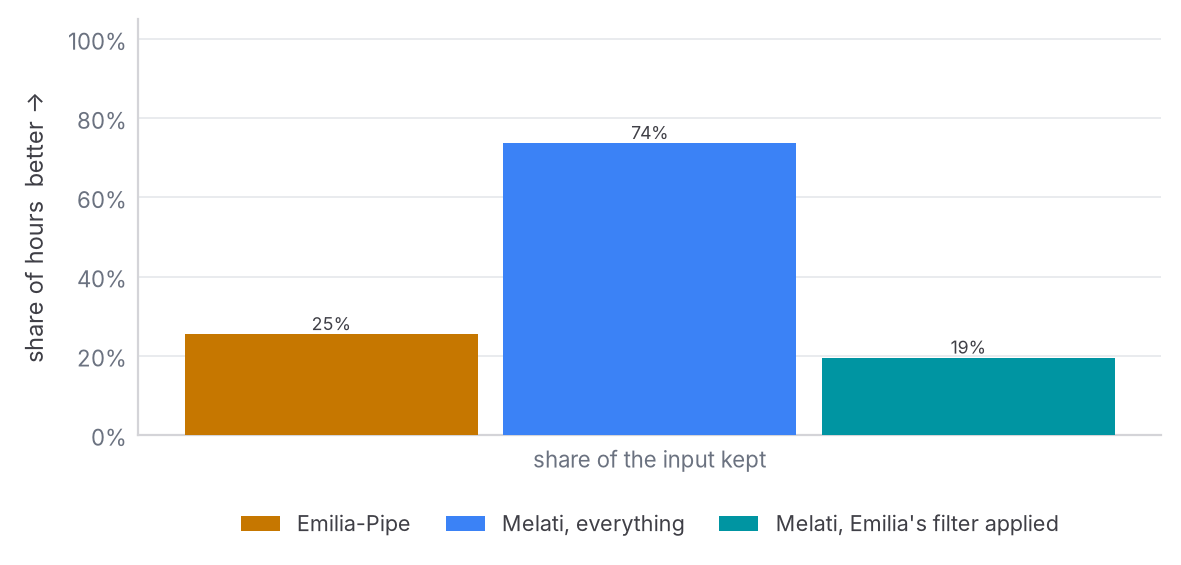
\includegraphics[width=0.8\linewidth]{img/fig_pil_yield.png}
\caption{Hours kept as a share of the input, 200 Malaysian podcasts.}
\label{fig:pilyield}
\end{figure}

Upstream writes MP3 at \val{pil/emilia/kbps} kbit/s, which cuts the spectrum at \val{pil/emilia/cutoff} kHz;
Melati writes FLAC, whose spectrum ends where the sources' does, at \val{pil/melati_all/cutoff} kHz. Upstream's
level normalisation leaves \val{pil/emilia/fullscale} of its segments at full scale and \val{pil/emilia/overfull}
past it; Melati none.

Words at the cut (Figure~\ref{fig:pilcut}): upstream starts inside a word in \val{pil/emilia/firstcut} of its
segments and Melati in \val{pil/melati_all/firstcut}; at the end the order flips, \val{pil/emilia/lastcut} against
\val{pil/melati_all/lastcut}. Podcast guests talk over each other far more than VoxConverse's speakers, and where
an overlap is cut out the speaker it interrupts is often mid-word even after the back-off; upstream keeps the
overlap, and with it the second voice.

\begin{figure}[H]
\centering
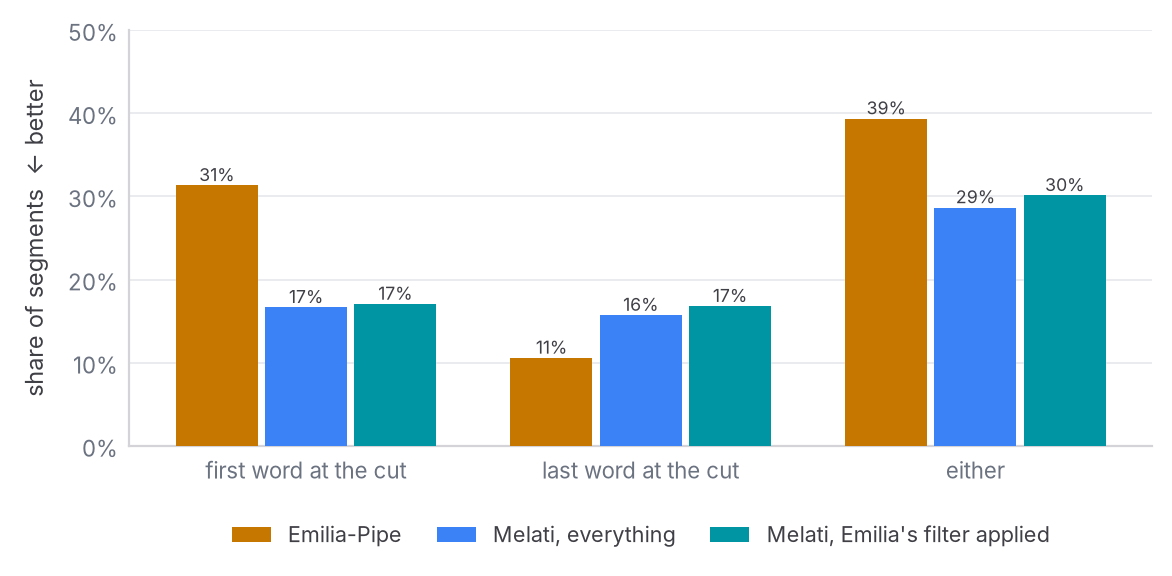
\includegraphics[width=0.92\linewidth]{img/fig_pil_cut.png}
\caption{Segments whose first or last aligned word is within 20 ms of the cut, 200 Malaysian podcasts.}
\label{fig:pilcut}
\end{figure}

Of the laughs the event detector finds in the source recordings, \val{pil/melati_all/laugh_kept} are still audible
in Melati's export and \val{pil/emilia/laugh_kept} in upstream's, and Melati tags \val{pil/melati_all/laugh_tagged}
of them. English words make up \val{pil/melati_all/en_in_ms} of the words in Melati's Malay segments and
\val{pil/emilia/en_in_ms} in upstream's: neither forces a language, so neither translates the code-switching away.
Melati's segments are shorter (Figure~\ref{fig:pildur}), for the reasons they are on VoxConverse.

\begin{figure}[H]
\centering
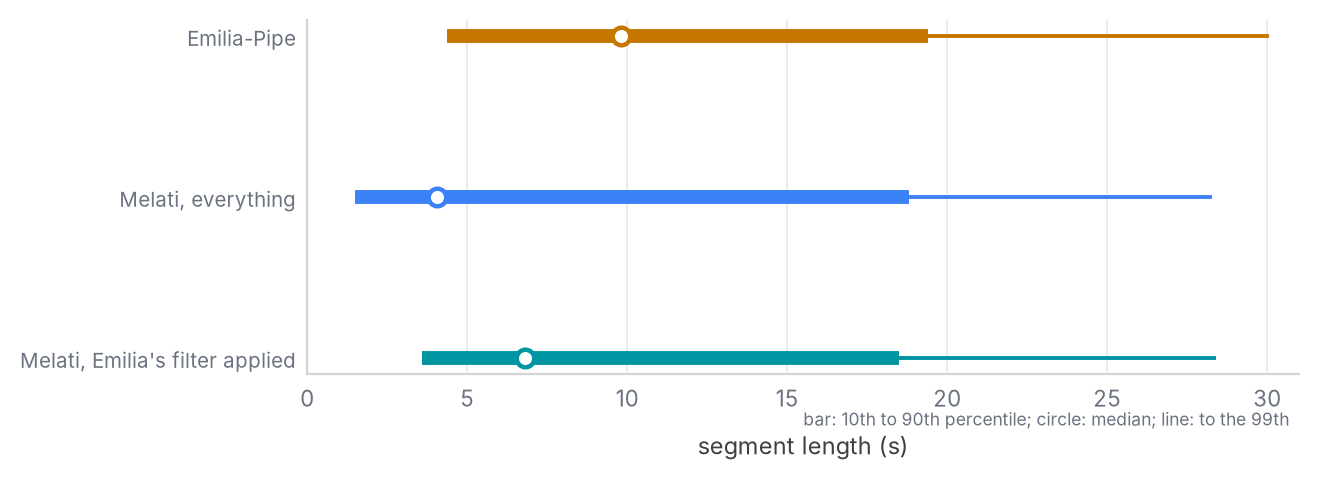
\includegraphics[width=0.86\linewidth]{img/fig_pil_dur.png}
\caption{Segment length per pipeline, 200 Malaysian podcasts.}
\label{fig:pildur}
\end{figure}

\section{Melati v1}
\label{sec:v1}
\label{sec:dataset}

\ifdscomplete
The whole podcast source went through the pipeline as described: \val{ds/src_recs} recordings,
\val{ds/src_h} hours (\val{ds/empty} of its files are empty). Melati v1 holds
\else
The run is under way: \val{ds/run/recs} of the source's \val{ds/src_recs} recordings (\val{ds/run/audio_h} hours)
have been through the pipeline so far, and the first \val{ds/shards} of Melati v1's \val{ds/blocks} shards are
published. Their \val{ds/recs} recordings (\val{ds/src_h} hours) hold
\fi
\val{ds/hours} hours in \val{ds/segments} segments, \val{ds/kept} of the input, from \val{ds/speakers} speakers counted per recording, or
per ten-minute window in the \val{ds/win/recs} recordings (\val{ds/win/h} hours) diarized in windows.
Malay is \val{ds/lang/ms/share} of the hours and English \val{ds/lang/en/share}. Left out are the
\val{ds/left/n} segments (\val{ds/left/h} hours, \val{ds/left/share} of all) whose transcript cannot be what was
said: Chinese and Tamil that Whisper did not hear itself (\val{ds/left/language_fallback/n}) or heard in a recording
mostly in another language (\val{ds/left/language_stray/n}), which on these podcasts is every one of them; text
mostly in a script its language is not written in (\val{ds/left/wrong_script/n}, Quranic Arabic labelled Malay or
English); and segments with no text (\val{ds/left/no_text/n}). No score is filtered on: the core of Emilia-Pipe's
filter (3 to 30 s, DNSMOS at least 3) would keep \val{ds/emilia/h} hours of it, and a column counts the words
aligned into under 25 ms, text the cut does not hold: two or more in \val{ds/squeezed} of the segments. It is published with the audio inline, under CC BY-NC 4.0 as its source
is, at \url{https://huggingface.co/datasets/Scicom-intl/Melati}.

Per hour of speech it tags \val{ds/ev/breathes/ph} breaths, \val{ds/ev/laughs/ph} laughs (\val{ds/laughs_over} of
them over someone's words), \val{ds/ev/coughs/ph} coughs, \val{ds/ev/sniffs/ph} sniffs and \val{ds/ev/throat/ph}
throat clearings, marks \val{ds/dlv/whisper/ph} whispered spans, and writes \val{ds/fill/ph} fillers
(Figure~\ref{fig:dstags}). Emotion spans run from \val{ds/emo/happy/ph} happy ones an hour to
\val{ds/emo/sad/ph} sad ones.
It also writes the sounds around the speech that its AudioSet tagger hears (Section~\ref{sec:astagger}):
\val{ds/snd/music/ph} \texttt{[music]} tags an hour, and \val{ds/snd/other/n} others in all
(\val{ds/snd/other/kinds}). Every segment also carries the tagger's labels as a column, and that column hears music
in \val{ds/snd/music_share} of the segments. \val{ds/snd/music_mix_share} of those are exported from the recording
itself. The separator runs only where PANNs hears background, so these keep their music, mostly faint under the
voice, and the column is how to leave them out.

\begin{figure}[H]
\centering
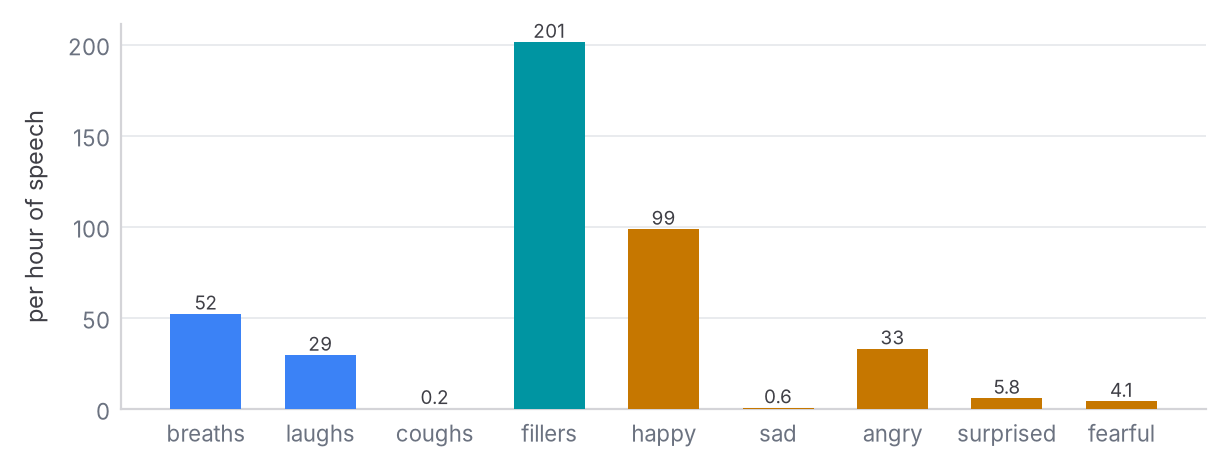
\includegraphics[width=0.92\linewidth]{img/fig_dataset_tags.png}
\caption{Melati v1's tags per hour of speech: non-verbal sounds (blue), fillers (teal), emotion spans (amber).}
\label{fig:dstags}
\end{figure}

\paragraph{What a whole corpus taught the servers.} \ifdscomplete The run took \else So far the run has taken \fi
\val{ds/run/wall_h} hours on six shared GPUs,
\val{ds/run/xrt} times realtime overall (Figure~\ref{fig:fullrun}). The pilot's 200 recordings never showed which
server a whole corpus waits on, and each fix moved the wait to the next one:
\begin{enumerate}
\item The w2v-BERT emotion head ran one clip at a time and was the slowest model in the tag server by far. Clips of
  similar length batched, masked and pooled over each clip's own frames are the same arithmetic: on
  \val{ds/ssl/clips} real clips the features agree at cosine \val{ds/ssl/cos} or better and the probabilities
  within \val{ds/ssl/p}, and it ran \val{ds/ssl/w2v} times faster (WavLM \val{ds/ssl/wavlm}).
\item Diarization reads a whole recording at once. Two long ones filled one server's KV cache while round-robin
  queued most of the waiting recordings behind them and its sibling had room. The client now sends each call to the
  replica with the fewest calls open, and diarization got two more replicas.
\item vLLM's default batch budget starts five Whisper encoder passes a step, and the filler stage transcribes every
  voiced gap alone, each a full 30-second pass. A larger budget and a third replica emptied its queue.
\item A diarization pass over 45 minutes holds 35 to 45\% of a server's KV cache while it decodes at tens of
  tokens a second. Three filled a replica and nothing behind them was admitted, so these passes outlasted the
  client's half-hour timeout and failed five tries in a row, and giving them longer made it worse: a slow recording
  keeps its place in the client, and every recording in flight ended up waiting on diarization. A recording over
  45 minutes is now ten-minute windows, and a shorter pass that gets no answer in two tries is too.
\end{enumerate}

\begin{figure}[H]
\centering
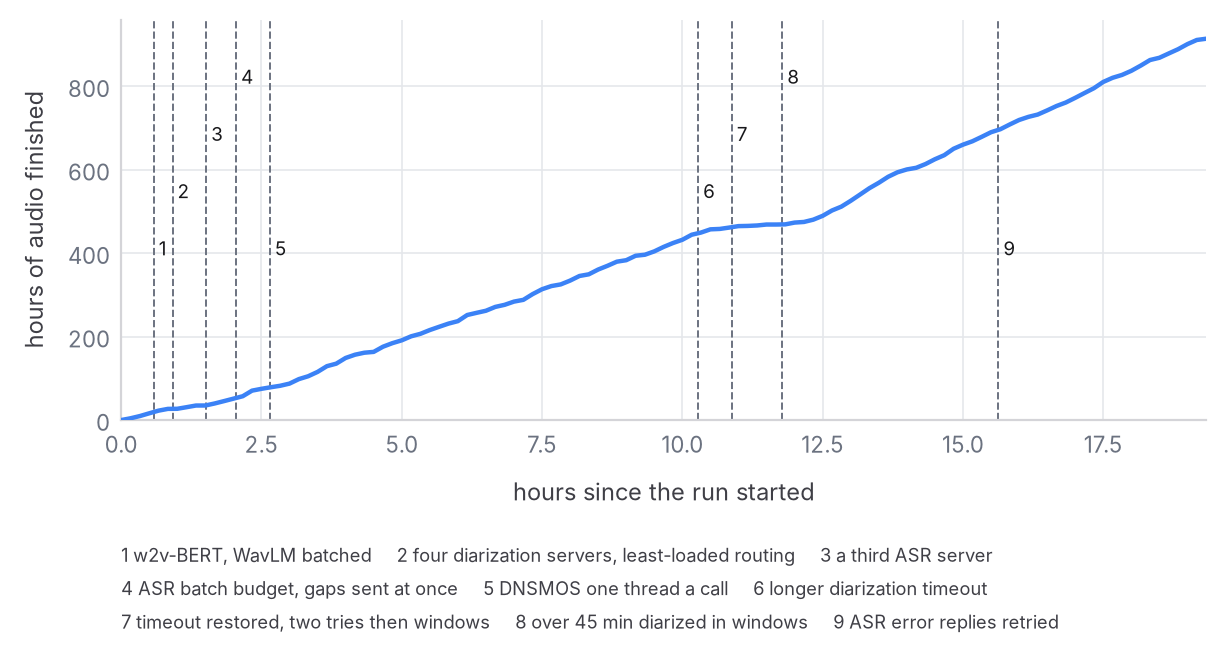
\includegraphics[width=0.92\linewidth]{img/fig_full_run.png}
\caption{Hours of audio finished against hours of running, on six shared GPUs. Dashed: the changes made while it
ran.}
\label{fig:fullrun}
\end{figure}

\section{Limitations}

No held-out emotion or non-verbal labels in Malay exist that we know of: every threshold was chosen on English and
Polish speech, and the podcast rates behind the emotion thresholds are assumptions until the labelling set is
labelled. Laughter two people share is overlap and is cut out. The released transcriber returns nothing for \val{asr/merge/my_empty} of Malaysian clips and more of
noisy speech, and still writes over \val{asr/merge/wild_words} of real voice-free audio; the merge was chosen on the
arms that separate the fine-tunes, which a held-out set would make firmer. Purity is measured on VoxConverse, which
is not Malaysian. Throughput was measured on shared GPUs only. The fine-tune's training audio includes Malaysian
podcast speech licensed for non-commercial use, and so is the checkpoint.

\section{Conclusion}

What a speech dataset keeps between the words decides what a generator trained on it can do. Melati keeps the
laughs, fillers and emotion of podcast speech where it can show they are right, and keeps the audio whole. The
transcriber it needed taught a second lesson: a model allowed to stop has to be measured where it is allowed to
stop, or the benchmark grades the decoder's constraints instead of the model.

\section*{Acknowledgement}

We thank Scicom (MSC) Berhad for the compute and the time to build this.

\bibliographystyle{plainnat}
\bibliography{neurips_2023}

\end{document}
